\documentclass{fast-nuces-bs}
%\documentclass{article}

\usepackage{blindtext}
\usepackage{mathptmx}% Times Roman font
\usepackage[T1]{fontenc}
\usepackage{lipsum} 
\usepackage{sectsty}
\usepackage{tikz-uml}
\usepackage{graphicx}
\usepackage{pdflscape}
\usepackage{longtable}
\usepackage{array}
\usepackage{booktabs}
% =============================================================================
% UNIFY -- shared TikZ styles for the SE diagrams
% Load ONCE in the report preamble (main.tex), after \usepackage{tikz-uml}:
%     % =============================================================================
% UNIFY -- shared TikZ styles for the SE diagrams
% Load ONCE in the report preamble (main.tex), after \usepackage{tikz-uml}:
%     % =============================================================================
% UNIFY -- shared TikZ styles for the SE diagrams
% Load ONCE in the report preamble (main.tex), after \usepackage{tikz-uml}:
%     \input{diagrams/unify-diagram-styles}
% Plain TikZ only (no tikz-uml dependency), so it compiles on any TeX Live.
% =============================================================================
\usepackage{tikz}
\usetikzlibrary{arrows.meta,positioning,calc,fit,backgrounds,
                shapes.geometric,shapes.multipart,decorations.pathreplacing}

% ---- palette (prints legibly in greyscale) ----------------------------------
\definecolor{uInk}{HTML}{1F2933}
\definecolor{uMuted}{HTML}{5B6670}
\definecolor{uLine}{HTML}{3E4C59}
\definecolor{uIngest}{HTML}{D9E8F5}   % event reliability / version store
\definecolor{uGraph}{HTML}{DDEFDF}    % evidence graph / policy / traceability
\definecolor{uVerify}{HTML}{F6E6CF}   % verification / findings
\definecolor{uIntent}{HTML}{E7E1F3}   % intent-side artifacts
\definecolor{uOk}{HTML}{2F7D4E}
\definecolor{uWarn}{HTML}{B7791F}
\definecolor{uBad}{HTML}{B4372F}
\definecolor{uSpan}{HTML}{FCE9A6}

% ---- fixed font sizes, so layouts don't break in 11pt/12pt report classes ----
\newcommand{\uDiagScript}{\fontsize{7pt}{8.5pt}\selectfont}
\newcommand{\uDiagSmall}{\fontsize{9pt}{11pt}\selectfont}
\newcommand{\uDiagNormal}{\fontsize{10pt}{12pt}\selectfont}

\tikzset{
  % ---- generic ---------------------------------------------------------------
  every picture/.append style={line join=round,
     execute at begin picture={\let\scriptsize\uDiagScript
       \let\small\uDiagSmall\let\normalsize\uDiagNormal\uDiagSmall}},
  every node/.append style={execute at begin node={\hyphenpenalty=10000\exhyphenpenalty=10000}},
  uline/.style={draw=uLine, line width=0.6pt},
  lbl/.style={font=\scriptsize, text=uMuted, fill=white, inner sep=1pt},
  note/.style={draw=uMuted, fill=yellow!8, font=\scriptsize, align=left,
               text width=#1, inner sep=4pt, rounded corners=1pt},
  note/.default=4.6cm,
  % ---- use-case --------------------------------------------------------------
  usecase/.style={ellipse, draw=uLine, fill=white, line width=0.6pt,
                  minimum width=4.4cm, minimum height=0.95cm, align=center,
                  font=\scriptsize, inner sep=1pt, text width=3.6cm},
  sysboundary/.style={draw=uLine, line width=0.9pt, rounded corners=3pt,
                      fill=uIngest!25},
  assoc/.style={draw=uLine, line width=0.5pt},
  stereo/.style={draw=uLine, line width=0.5pt, dashed,
                 -{Stealth[length=2mm]}},
  extsys/.style={draw=uLine, fill=uGraph!60, rounded corners=2pt,
                 minimum width=2.3cm, minimum height=0.8cm, font=\scriptsize,
                 align=center},
  % ---- ERD / class boxes -------------------------------------------------------
  table/.style={rectangle split, rectangle split parts=2, draw=uLine,
                line width=0.6pt, rectangle split part fill={#1,white},
                text width=4.9cm, align=left, inner sep=3pt,
                font=\scriptsize\ttfamily},
  table/.default=uGraph,
  klass/.style={rectangle split, rectangle split parts=2, draw=uLine,
                line width=0.6pt, rectangle split part fill={#1,white},
                text width=3.7cm, align=center, inner sep=3pt,
                font=\scriptsize},
  klass/.default=white,
  rel/.style={draw=uLine, line width=0.55pt},
  card/.style={font=\scriptsize\bfseries, text=uInk, inner sep=1.5pt},
  generalise/.style={draw=uLine, line width=0.6pt,
                     -{Triangle[open, length=3mm, width=3mm]}},
  directed/.style={draw=uLine, line width=0.55pt, -{Stealth[length=2.2mm]}},
  % ---- flow ----------------------------------------------------------------------
  decision/.style={diamond, aspect=1.9, draw=uLine, fill=white,
                   line width=0.6pt, font=\scriptsize, align=center,
                   inner sep=1pt, text width=2.1cm},
  step/.style={rectangle, rounded corners=2pt, draw=uLine, line width=0.6pt,
               font=\scriptsize, align=center, minimum height=0.8cm,
               text width=#1, inner sep=3pt},
  step/.default=2.6cm,
  flow/.style={draw=uLine, line width=0.6pt, -{Stealth[length=2.2mm]}},
}

% ---- stick-figure actor:  \actor{name}{(x,y)}{Label} ---------------------------
\newcommand{\actor}[3]{%
  \begin{scope}[shift={#2}, line width=0.8pt, draw=uInk]
    \draw (0,0.62) circle (0.17);
    \draw (0,0.45) -- (0,-0.05);
    \draw (-0.32,0.28) -- (0.32,0.28);
    \draw (0,-0.05) -- (-0.24,-0.45);
    \draw (0,-0.05) -- (0.24,-0.45);
    \node[font=\scriptsize\bfseries, align=center, anchor=north]
         (#1-label) at (0,-0.5) {#3};
    \coordinate (#1) at (0.4,0.2);
  \end{scope}}

% Plain TikZ only (no tikz-uml dependency), so it compiles on any TeX Live.
% =============================================================================
\usepackage{tikz}
\usetikzlibrary{arrows.meta,positioning,calc,fit,backgrounds,
                shapes.geometric,shapes.multipart,decorations.pathreplacing}

% ---- palette (prints legibly in greyscale) ----------------------------------
\definecolor{uInk}{HTML}{1F2933}
\definecolor{uMuted}{HTML}{5B6670}
\definecolor{uLine}{HTML}{3E4C59}
\definecolor{uIngest}{HTML}{D9E8F5}   % event reliability / version store
\definecolor{uGraph}{HTML}{DDEFDF}    % evidence graph / policy / traceability
\definecolor{uVerify}{HTML}{F6E6CF}   % verification / findings
\definecolor{uIntent}{HTML}{E7E1F3}   % intent-side artifacts
\definecolor{uOk}{HTML}{2F7D4E}
\definecolor{uWarn}{HTML}{B7791F}
\definecolor{uBad}{HTML}{B4372F}
\definecolor{uSpan}{HTML}{FCE9A6}

% ---- fixed font sizes, so layouts don't break in 11pt/12pt report classes ----
\newcommand{\uDiagScript}{\fontsize{7pt}{8.5pt}\selectfont}
\newcommand{\uDiagSmall}{\fontsize{9pt}{11pt}\selectfont}
\newcommand{\uDiagNormal}{\fontsize{10pt}{12pt}\selectfont}

\tikzset{
  % ---- generic ---------------------------------------------------------------
  every picture/.append style={line join=round,
     execute at begin picture={\let\scriptsize\uDiagScript
       \let\small\uDiagSmall\let\normalsize\uDiagNormal\uDiagSmall}},
  every node/.append style={execute at begin node={\hyphenpenalty=10000\exhyphenpenalty=10000}},
  uline/.style={draw=uLine, line width=0.6pt},
  lbl/.style={font=\scriptsize, text=uMuted, fill=white, inner sep=1pt},
  note/.style={draw=uMuted, fill=yellow!8, font=\scriptsize, align=left,
               text width=#1, inner sep=4pt, rounded corners=1pt},
  note/.default=4.6cm,
  % ---- use-case --------------------------------------------------------------
  usecase/.style={ellipse, draw=uLine, fill=white, line width=0.6pt,
                  minimum width=4.4cm, minimum height=0.95cm, align=center,
                  font=\scriptsize, inner sep=1pt, text width=3.6cm},
  sysboundary/.style={draw=uLine, line width=0.9pt, rounded corners=3pt,
                      fill=uIngest!25},
  assoc/.style={draw=uLine, line width=0.5pt},
  stereo/.style={draw=uLine, line width=0.5pt, dashed,
                 -{Stealth[length=2mm]}},
  extsys/.style={draw=uLine, fill=uGraph!60, rounded corners=2pt,
                 minimum width=2.3cm, minimum height=0.8cm, font=\scriptsize,
                 align=center},
  % ---- ERD / class boxes -------------------------------------------------------
  table/.style={rectangle split, rectangle split parts=2, draw=uLine,
                line width=0.6pt, rectangle split part fill={#1,white},
                text width=4.9cm, align=left, inner sep=3pt,
                font=\scriptsize\ttfamily},
  table/.default=uGraph,
  klass/.style={rectangle split, rectangle split parts=2, draw=uLine,
                line width=0.6pt, rectangle split part fill={#1,white},
                text width=3.7cm, align=center, inner sep=3pt,
                font=\scriptsize},
  klass/.default=white,
  rel/.style={draw=uLine, line width=0.55pt},
  card/.style={font=\scriptsize\bfseries, text=uInk, inner sep=1.5pt},
  generalise/.style={draw=uLine, line width=0.6pt,
                     -{Triangle[open, length=3mm, width=3mm]}},
  directed/.style={draw=uLine, line width=0.55pt, -{Stealth[length=2.2mm]}},
  % ---- flow ----------------------------------------------------------------------
  decision/.style={diamond, aspect=1.9, draw=uLine, fill=white,
                   line width=0.6pt, font=\scriptsize, align=center,
                   inner sep=1pt, text width=2.1cm},
  step/.style={rectangle, rounded corners=2pt, draw=uLine, line width=0.6pt,
               font=\scriptsize, align=center, minimum height=0.8cm,
               text width=#1, inner sep=3pt},
  step/.default=2.6cm,
  flow/.style={draw=uLine, line width=0.6pt, -{Stealth[length=2.2mm]}},
}

% ---- stick-figure actor:  \actor{name}{(x,y)}{Label} ---------------------------
\newcommand{\actor}[3]{%
  \begin{scope}[shift={#2}, line width=0.8pt, draw=uInk]
    \draw (0,0.62) circle (0.17);
    \draw (0,0.45) -- (0,-0.05);
    \draw (-0.32,0.28) -- (0.32,0.28);
    \draw (0,-0.05) -- (-0.24,-0.45);
    \draw (0,-0.05) -- (0.24,-0.45);
    \node[font=\scriptsize\bfseries, align=center, anchor=north]
         (#1-label) at (0,-0.5) {#3};
    \coordinate (#1) at (0.4,0.2);
  \end{scope}}

% Plain TikZ only (no tikz-uml dependency), so it compiles on any TeX Live.
% =============================================================================
\usepackage{tikz}
\usetikzlibrary{arrows.meta,positioning,calc,fit,backgrounds,
                shapes.geometric,shapes.multipart,decorations.pathreplacing}

% ---- palette (prints legibly in greyscale) ----------------------------------
\definecolor{uInk}{HTML}{1F2933}
\definecolor{uMuted}{HTML}{5B6670}
\definecolor{uLine}{HTML}{3E4C59}
\definecolor{uIngest}{HTML}{D9E8F5}   % event reliability / version store
\definecolor{uGraph}{HTML}{DDEFDF}    % evidence graph / policy / traceability
\definecolor{uVerify}{HTML}{F6E6CF}   % verification / findings
\definecolor{uIntent}{HTML}{E7E1F3}   % intent-side artifacts
\definecolor{uOk}{HTML}{2F7D4E}
\definecolor{uWarn}{HTML}{B7791F}
\definecolor{uBad}{HTML}{B4372F}
\definecolor{uSpan}{HTML}{FCE9A6}

% ---- fixed font sizes, so layouts don't break in 11pt/12pt report classes ----
\newcommand{\uDiagScript}{\fontsize{7pt}{8.5pt}\selectfont}
\newcommand{\uDiagSmall}{\fontsize{9pt}{11pt}\selectfont}
\newcommand{\uDiagNormal}{\fontsize{10pt}{12pt}\selectfont}

\tikzset{
  % ---- generic ---------------------------------------------------------------
  every picture/.append style={line join=round,
     execute at begin picture={\let\scriptsize\uDiagScript
       \let\small\uDiagSmall\let\normalsize\uDiagNormal\uDiagSmall}},
  every node/.append style={execute at begin node={\hyphenpenalty=10000\exhyphenpenalty=10000}},
  uline/.style={draw=uLine, line width=0.6pt},
  lbl/.style={font=\scriptsize, text=uMuted, fill=white, inner sep=1pt},
  note/.style={draw=uMuted, fill=yellow!8, font=\scriptsize, align=left,
               text width=#1, inner sep=4pt, rounded corners=1pt},
  note/.default=4.6cm,
  % ---- use-case --------------------------------------------------------------
  usecase/.style={ellipse, draw=uLine, fill=white, line width=0.6pt,
                  minimum width=4.4cm, minimum height=0.95cm, align=center,
                  font=\scriptsize, inner sep=1pt, text width=3.6cm},
  sysboundary/.style={draw=uLine, line width=0.9pt, rounded corners=3pt,
                      fill=uIngest!25},
  assoc/.style={draw=uLine, line width=0.5pt},
  stereo/.style={draw=uLine, line width=0.5pt, dashed,
                 -{Stealth[length=2mm]}},
  extsys/.style={draw=uLine, fill=uGraph!60, rounded corners=2pt,
                 minimum width=2.3cm, minimum height=0.8cm, font=\scriptsize,
                 align=center},
  % ---- ERD / class boxes -------------------------------------------------------
  table/.style={rectangle split, rectangle split parts=2, draw=uLine,
                line width=0.6pt, rectangle split part fill={#1,white},
                text width=4.9cm, align=left, inner sep=3pt,
                font=\scriptsize\ttfamily},
  table/.default=uGraph,
  klass/.style={rectangle split, rectangle split parts=2, draw=uLine,
                line width=0.6pt, rectangle split part fill={#1,white},
                text width=3.7cm, align=center, inner sep=3pt,
                font=\scriptsize},
  klass/.default=white,
  rel/.style={draw=uLine, line width=0.55pt},
  card/.style={font=\scriptsize\bfseries, text=uInk, inner sep=1.5pt},
  generalise/.style={draw=uLine, line width=0.6pt,
                     -{Triangle[open, length=3mm, width=3mm]}},
  directed/.style={draw=uLine, line width=0.55pt, -{Stealth[length=2.2mm]}},
  % ---- flow ----------------------------------------------------------------------
  decision/.style={diamond, aspect=1.9, draw=uLine, fill=white,
                   line width=0.6pt, font=\scriptsize, align=center,
                   inner sep=1pt, text width=2.1cm},
  step/.style={rectangle, rounded corners=2pt, draw=uLine, line width=0.6pt,
               font=\scriptsize, align=center, minimum height=0.8cm,
               text width=#1, inner sep=3pt},
  step/.default=2.6cm,
  flow/.style={draw=uLine, line width=0.6pt, -{Stealth[length=2.2mm]}},
}

% ---- stick-figure actor:  \actor{name}{(x,y)}{Label} ---------------------------
\newcommand{\actor}[3]{%
  \begin{scope}[shift={#2}, line width=0.8pt, draw=uInk]
    \draw (0,0.62) circle (0.17);
    \draw (0,0.45) -- (0,-0.05);
    \draw (-0.32,0.28) -- (0.32,0.28);
    \draw (0,-0.05) -- (-0.24,-0.45);
    \draw (0,-0.05) -- (0.24,-0.45);
    \node[font=\scriptsize\bfseries, align=center, anchor=north]
         (#1-label) at (0,-0.5) {#3};
    \coordinate (#1) at (0.4,0.2);
  \end{scope}}

\usepackage{titlesec}

% ---------------------------------------------------------------------------
% Citation style
%
% fast-nuces-bs.cls loads natbib with [sort, numbers, authoryear] -- the last
% two options contradict each other. Left alone, the outcome depends on which
% .bst bibtex happens to run, and plain IEEEtran emits numeric \bibitem
% entries that natbib then rejects with "Bibliography not compatible with
% author-year citations". Author-year is pinned here explicitly and paired
% with IEEEtranN at \bibliographystyle, which is IEEEtran's natbib-compatible
% variant. Citations therefore render "De Lucia et al. (2007)" -- the same
% author-year form the submitted build used, though IEEEtranN sets the
% delimiter to parentheses rather than the square brackets the earlier build
% produced, which is cosmetic and does not affect the entries themselves.
% \AtBeginDocument because IEEEtranN sets up its own author-year citations
% when it loads, and a preamble-only call is overwritten by that.
% ---------------------------------------------------------------------------
\AtBeginDocument{\setcitestyle{authoryear}}

% ---------------------------------------------------------------------------
% Front-matter pagination
%
% fast-nuces-bs.cls emits the table of contents, list of figures and list of
% tables from inside \maketitle, and then switches the page counter to arabic
% and resets it to zero. That numbers the contents pages 2..10 -- so the tenth
% front-matter page prints a bare "0" -- and places them ahead of the
% declarations and the abstract, which are roman-numbered. Patch those five
% statements out of \maketitle: main.tex emits the ToC/LoF/LoT itself, in
% roman, immediately before Chapter 1.
% ---------------------------------------------------------------------------
\patchcmd{\maketitle}{\tableofcontents}{}{}{}
\patchcmd{\maketitle}{\listoffigures}{}{}{}
\patchcmd{\maketitle}{\listoftables}{}{}{}
\patchcmd{\maketitle}{\pagenumbering{arabic}}{}{}{}
\patchcmd{\maketitle}{\setcounter{page}{0}}{}{}{}

% Every list that opens on a fresh right-hand page needs its ToC entry
% written only after the page break has happened, or the recorded page number
% points at the previous page. \cleardoublepage, not \clearpage: with a
% two-sided book class \chapter* starts on an odd page and may skip a blank
% verso, so a plain \clearpage records the page before the heading.
\newcommand{\listintoc}[1]{%
	\cleardoublepage
	\phantomsection
	\addcontentsline{toc}{chapter}{#1}%
}

% Information about the Thesis 
% -----------------------------------------------------------------------------
% (All are compulsory, do not delete any line other than author Information)
% For e.g., usually there are 3 students in a group, so leave authorone, 
% authortwo, and authorthree, and delete authorfour.
%%%%%%%%%%%%%%%%%%%%%%%%%%%%%%%%%%%%%%%%%%%%%%%%%%%%%%%%%%%%%%%%%%%%%%%%%%%%%%%
% Single source of truth for the team roster. The title page (\authorone...)
% and the Students' Submission signature page (\studentone...) both read from
% these, so the two can never drift apart.
\newcommand{\projecttitle}{UNIFY: Cross-Tool Change Assurance for Product Teams}
\newcommand{\memberI}{Abdullah Amin}
\newcommand{\rollI}{23i-0691}
\newcommand{\memberII}{Haaniah Ismail}
\newcommand{\rollII}{23i-0605}
\newcommand{\memberIII}{Mishal Fatima}
\newcommand{\rollIII}{23i-0776}
\newcommand{\studentone}{\memberI\ (\rollI)}
\newcommand{\studenttwo}{\memberII\ (\rollII)}
\newcommand{\studentthree}{\memberIII\ (\rollIII)}
%%%%%%%%%%%%%%%%%%%%%%%%%%%%%%%%%%%%%%%%%%%%%%%%%%%%%%%%%%%%%%%%%%%%%%%%%%%%%%%
\department{FAST School of Computing}
\faculty{Computer Science}
\degreeyear{2026}
\degreemonth{October}
\degreename{Computer Science}
\campuscity{Islamabad}
\authorone{\memberI}{\rollI}
\authortwo{\memberII}{\rollII}
\authorthree{\memberIII}{\rollIII}
\supervisor{Dr. Ali Zeeshan Ijaz}
\sessionduration{2023-2027}
% No co-supervisor on this project: delete the line below to keep it off the
% title page (the class prints a "Co-Supervised by" block whenever it is set).
%\cosupervisor{Mr./ Ms./ Dr. Supervisor Name (please remove if not applicable)}
\deanname{Dr. Dean Computing}
\directorname{Dr. Director of the Campus}
\hodname{Dr. Head of Computer Science Department}
\fypcoordinatorname{Name of FYP Coordinator}
\title{\projecttitle}
%%%%%%%%%%%%%%%%%%%%%%%%%%%%%%%%%%%%%%%%%%%%%%%%%%%%%%%%%%%%%%%%%%%%%%%%%%%%%%%

%%%%%%%%%%%%%%%%%%%%%%%%%%%%%%%%%%%%%%%%%%%%%%%%%%%%%%%%%%%%%%%%%%%%%%%%%%%%%%
% Former document starts below this
\begin{document}

%\begin{acknowledgements}
%	Your acknowledgments here
%\end{acknowledgements}

%\begin{abstract}
%Briefly state the (1) research problem, (2) methodology, (3) key results, and (4) conclusion. Generally, abstracts are between 150 and 200 words–roughly 10-15 sentences.
%\end{abstract}

\cleardoublepage
\pagenumbering{roman}
\chapter*{Students' Submission}
\addcontentsline{toc}{chapter}{Students' Submission}
We certify that this report is submitted as the FYP-1 mid-report for the project titled \textit{\projecttitle}.

\vspace{1.5cm}
\noindent
\begin{tabular}{@{}>{\raggedright\arraybackslash}p{0.52\textwidth}@{\hspace{0.04\textwidth}}>{\raggedright\arraybackslash}p{0.40\textwidth}@{}}
Student 1: \studentone & Signature: \hrulefill\\[1.4cm]
Student 2: \studenttwo & Signature: \hrulefill\\[1.4cm]
Student 3: \studentthree & Signature: \hrulefill
\end{tabular}

\chapter*{Anti-Plagiarism Statement}
\addcontentsline{toc}{chapter}{Anti-Plagiarism Statement}
The students certify that this report is their own work and that all sources used in preparing the report have been appropriately acknowledged and referenced.

\chapter*{Authors' Declaration}
\addcontentsline{toc}{chapter}{Authors' Declaration}
We declare that the work documented in this report represents the work completed by the project team up to the FYP-1 mid-report stage. Contributions, tools, external components, and relevant sources are disclosed where applicable.

\chapter*{Abstract}
\addcontentsline{toc}{chapter}{Abstract}

A software team records one unit of work across three tools --- a design file, a
ticket and a repository --- and none of them holds the relationship between the
others, so a reviewer must reconstruct by hand, across several interfaces,
whether a proposed change still matches the intent it claims to implement. This
report presents UNIFY, a locally deployable change-assurance system that
reconciles asynchronous events from those tools into a versioned evidence graph
and, for each atomic acceptance criterion, assembles a bounded evidence packet,
runs a fixed-pass local verification loop over it, and passes the result through
a deterministic gate that resolves every citation against the stored packet.
Outcomes are restricted to supported, contradicted, partial or insufficient
evidence, so abstention is a first-class result rather than a failure. Research
against comparable products established that criterion-level checking already
ships commercially; the differentiators claimed here are versioned provenance,
deterministic gating, event reconciliation and local execution, each of which is
measurable. At this evaluation the requirements, design, twelve diagrams,
nineteen-route reviewer surface and a fifteen-case annotated data pilot exist
and are verified by the checks reported in Chapter~8; the ingestion, evidence
graph and verification layers remain to be built in FYP-2.

\chapter*{Acknowledgments}
\addcontentsline{toc}{chapter}{Acknowledgments}
The project team acknowledges the guidance and support received from the project supervisor, faculty members, and other contributors.

\chapter*{Executive Summary}
\addcontentsline{toc}{chapter}{Executive Summary}

\section*{The problem}

Product teams deliberately use separate tools for design, requirements and
implementation, because each is better at its own task than a combined product
would be. The cost is that the relationships between their contents exist only
in the heads of the people doing the work. When a designer moves a screen after
the code was written, or a ticket is closed while the implementation is still
changing, no artifact notices. The failure surfaces in a code review, where a
reviewer must decide whether one pull request still matches the intent it
claims to implement --- a judgement formed across several interfaces, from
memory, with nothing recording what evidence supported it. The reasoning is lost
the moment the change is merged.

\section*{What UNIFY does}

UNIFY subscribes to one design source, one work-item source and one change
source, normalises their events into a single envelope, and stores every
artifact version as an immutable snapshot. Relationships between artifacts are
persisted as typed edges that record how they were established and how confident
the resolver was, so an explicit reference in a pull request title is
distinguishable in the data from an unconfirmed inference. For each atomic
acceptance criterion the system assembles a bounded evidence packet
deterministically, runs a fixed-pass local verification loop over it, and passes
the structured result through a deterministic gate that resolves every citation
against the stored packet. A verdict whose citations do not resolve is
downgraded, and the reason is recorded. The output vocabulary is closed ---
supported, contradicted, partial, or insufficient evidence --- with freshness
and review-required carried as separate fields. All inference runs on
infrastructure the team operates; no repository, ticket or design content is
transmitted to a hosted model interface.

\section*{Research position}

Chapter~2 reviews the comparable systems from their own documentation. CodeRabbit
pulls Jira issue context into a pull request review and returns addressed, not
addressed or unclear per linked objective; Atlassian's Rovo Dev compares a pull
request against the acceptance criteria of a linked Jira work item. Both overlap
directly with part of this project, both are hosted, and neither preserves the
versioned evidence behind a conclusion. The overlap is therefore conceded: the
claimed differentiators are local execution, versioned provenance across tools,
deterministic gating, and reconciliation of late, duplicated and out-of-order
events. Prior research in requirements traceability and automated code review,
and public evaluation corpora, are cited for what they establish rather than
borrowed for authority.

\section*{Status at this evaluation}

\begin{longtable}{p{0.34\textwidth} p{0.22\textwidth} p{0.38\textwidth}}
\caption{Status of the iteration 1 deliverables at the mid evaluation.}\label{tab:exec-status}\\
\hline\textbf{Area} & \textbf{State} & \textbf{Evidence} \\
\hline\endfirsthead
\hline\textbf{Area} & \textbf{State} & \textbf{Evidence} \\
\hline\endhead
Requirements baseline & Complete & 29 functional and 14 non-functional
  requirements, acceptance check per requirement (Ch.~4) \\
Design baseline & Complete & Layered architecture, components, data flow,
  domain model, ERD, verifier loop, anchoring and autonomy-ladder diagrams
  (Ch.~5) \\
Reviewer surface & Complete against typed mock data & 19 routes; typecheck, lint
  and production build pass; 29 static pages generated (Ch.~6) \\
Evaluation-data pilot & Protocol working, annotation incomplete & 15 cases from
  3 TypeScript/React repositories; 138 integrity checks, 0 failures; second
  annotation sheet pending (Ch.~8) \\
Ingestion, evidence graph, rules & Not started & Declared honestly in Ch.~6 and
  Ch.~8; sequenced in Ch.~10 \\
Verifier, gate, local model & Not started & No model downloaded; hardware risk
  still open \\
Process evidence & Maintained & 65 commits, 6 merged pull requests, per-member
  artefacts recorded, GenAI register maintained (Ch.~9) \\
\hline\end{longtable}

\section*{Risks and what comes next}

Three risks carry into the second year. Local inference has never been measured
on this team's hardware, so the ceiling on verification quality is unknown and
the spike is scheduled as early as a stable packet exists. The reliability and
verification work has not started, which is reported as a declared variance
against the iteration plan rather than glossed. And the comparable products have
been read but not trialled, so that comparison rests on documentation until the
dated trials are recorded.

FYP-2 proceeds in dependency order: shared contracts, CI and containers; then
ingestion reliability proven by replay tests; then the evidence graph, analyser
and rules; then the packet builder, bounded verifier and provenance gate, with
the front end bound to the real API and the mock layer removed. Evaluation data
is frozen before any component is tuned against it, two hard gates (rejection of
uncited verdicts, and run-to-run agreement) are enforced before any metric is
reported, and the fine-tuning experiment is decided by a rule written in advance,
so a negative result is reported as such. The frozen scope list in the team
checklist --- no new integrations, no autonomous write-back, no hosted model in
the committed system, no visual certification --- remains in force.

\chapter*{List of Abbreviations}
\addcontentsline{toc}{chapter}{List of Abbreviations}
\begin{longtable}{@{}>{\raggedright\arraybackslash}p{0.18\textwidth}>{\raggedright\arraybackslash}p{0.76\textwidth}@{}}
API & Application Programming Interface\\
AST & Abstract Syntax Tree\\
CI & Continuous Integration\\
CSV & Comma-Separated Values\\
DEI & Diversity, Equity and Inclusion\\
ERD & Entity-Relationship Diagram\\
FR & Functional Requirement\\
FYP & Final Year Project\\
GenAI & Generative Artificial Intelligence\\
HMAC & Hash-based Message Authentication Code\\
HTTP & Hypertext Transfer Protocol\\
JSON & JavaScript Object Notation\\
LLM & Large Language Model\\
NFR & Non-Functional Requirement\\
OAuth & Open Authorization\\
PM & Product Manager\\
PR & Pull Request\\
REST & Representational State Transfer\\
RLS & Row-Level Security\\
RPC & Remote Procedure Call\\
SDK & Software Development Kit\\
SHA & Secure Hash Algorithm\\
SQL & Structured Query Language\\
TC & Test Case\\
UC & Use Case\\
UI & User Interface\\
URL & Uniform Resource Locator\\
\end{longtable}


% Contents and the two lists, still in the roman front matter. \listintoc
% writes each entry only once the page break has happened, so the page
% numbers recorded in the .toc match the page the heading lands on.
\tableofcontents
\listintoc{\listfigurename}
\listoffigures
\listintoc{\listtablename}
\listoftables

\cleardoublepage
\pagenumbering{arabic}
\chapter{Introduction and Project Vision}

\section{Project Overview}

Unify is a locally deployed system that checks whether a proposed code change
actually does what the ticket and design it claims to implement say it should,
and shows the code and tests that support that conclusion.

A software team's record of a single piece of work is normally scattered across
three tools. The intended appearance and behaviour live in a design tool. The
requirement and its workflow state live in an issue tracker. The implementation
lives in a repository. Each tool versions its own record independently and none
of them understands what a change in one implies for the others. Unify
subscribes to all three, resolves which records refer to the same unit of work,
stores them with their versions and their provenance, and evaluates each
proposed change against the intent it is linked to.

The output is not a score and not a recommendation to merge. For each acceptance
criterion, the system reports whether the available evidence supports it,
contradicts it, supports it only in part, or is insufficient to decide, and every
decisive finding is accompanied by the file, line range and artifact version it
was derived from. A finding that cannot cite its evidence is not shown as a
finding.

All model inference runs on infrastructure the team owns. No repository content,
ticket text or design data is transmitted to a third-party model interface.

\section{Problem Statement}

Work drifts out of alignment across the tools that hold it, and the
inconsistency is discovered late.

A designer updates a screen after the corresponding implementation has already
been written. A ticket is marked complete while the code that implements it is
still changing. A pull request is reviewed against acceptance criteria that were
edited after the branch was cut. In each case the individual tools are behaving
correctly: each has an accurate record of its own artifact. What is missing is
any representation of the relationship between those artifacts, and therefore
any mechanism by which a change to one can raise a question about another.

The concrete decision that fails is a code review. A reviewer opening a pull
request must determine whether the change still matches the intent it claims to
implement. Doing so requires opening the tracker for the acceptance criteria,
opening the design tool and checking whether the approved design has moved since
the branch was created, reading the diff, and forming a judgement about whether
the tests actually exercise the criterion in question. That reasoning is
performed from memory across several interfaces, and no artifact records what
evidence supported the decision, so it is lost the moment the change is merged.

The consequence is that mismatches surface during testing, at deployment, or in
a status meeting, after the cost of building the wrong thing has already been
incurred.

\section{Problem Context and Motivation}

The problem is a consequence of tool specialisation. Teams adopt a design tool,
an issue tracker and a version control platform because each is substantially
better at its own task than a single integrated product would be. The cost of
that choice is that the relationships between their contents exist only in the
heads of the people doing the work.

Existing integrations address a narrower problem than the one described here.
Field synchronisation tools copy values between systems but do not reason about
whether the copied values remain consistent with one another. Pairwise
integrations connect two specific tools and notify on change, but see neither the
code nor the tests. Recent commercial code-review assistants do compare a pull
request against a linked issue, which overlaps directly with part of this
project's scope; they operate as hosted services, they do not preserve the
versioned evidence behind a conclusion, and they do not treat uncertainty as a
reportable outcome.

To confirm that the problem is real rather than assumed, the team consulted a
practising senior software engineer about his team's workflow. Three findings
shaped the design. Relationships between pull requests and tickets are currently
tracked manually by technical leads. Implementations built against
subsequently-changed designs have occurred repeatedly and have caused
rework. And the team already receives more automated notifications than it
reads, so a system that raises alerts of uncertain accuracy will be disabled
rather than tuned.

That third finding is the one that most constrains the design. It establishes
that precision matters more than coverage, and it is the reason the system is
built to abstain when evidence is insufficient rather than to guess.

\section{Project Vision}

A reviewer should be able to answer the question ``does this change do what it
says'' from one place, with the evidence attached, and the system should say
plainly when it cannot answer rather than producing a confident guess.

The longer-term intent is that the reasoning behind a review decision stops
being ephemeral. Today it exists only while the reviewer holds it; afterwards
the repository records that a change was approved but not what was checked.
Unify produces a durable, versioned evidence case for each change, which means
the basis for a past decision can be re-read against the artifact versions that
were current when it was made.

\section{Project Objectives}

\begin{enumerate}
  \item Resolve the identity of a single unit of work across a design source, a
        work-item source and a change source, recording which version of each
        artifact a relationship was established against, and achieve high
        precision on links derived from explicit references.
  \item Process notifications from those sources such that duplicate and
        out-of-order delivery converge to the same final state, and an event
        the source never delivered is recovered by reconciliation rather than
        silently missed.
  \item Extract, for a declared set of languages, the changed files, symbols,
        dependency neighbourhood and test evidence associated with a proposed
        change.
  \item Verify each atomic acceptance criterion against a deterministically
        assembled evidence packet, using a bounded local inference loop, and
        return a structured verdict with cited evidence spans.
  \item Prevent any verdict whose citations cannot be resolved against the
        evidence packet from being presented as a decisive finding.
  \item Anchor functional requirements to specific symbols and line ranges,
        pinned to a commit, and maintain those anchors as the code changes,
        reporting the proportion that survive.
  \item Evaluate the system against a manually constructed and independently
        labelled set of cases, and against stated baselines including the
        current manual workflow, reporting performance per class rather than as
        a single aggregate.
\end{enumerate}

\section{Project Scope}

\subsection*{Included}

Read-only ingestion from one design-intent source, one work-item source and one
change source. Deterministic and manually confirmed linking across those
sources. An immutable, versioned artifact store. A typed evidence graph carrying
provenance on every relationship. Deterministic policies covering design-version
drift, workflow-state inconsistency, overlapping change scope and
requirement--implementation divergence. Code and test analysis for the declared
languages. Criterion decomposition and deterministic context assembly. A bounded
local verification loop. A deterministic verdict and provenance gate. A reviewer
interface presenting evidence cases with resolution and audit history.
Role-based routing of findings and outbound delivery to one channel.

\subsection*{Excluded}

Autonomous code generation or repair. Any claim of general program correctness.
Support for languages beyond those declared. Unrestricted conversational
interaction with the system. Two-way write-back of data to the source systems.
Any hosted model interface in the committed system. Pixel-level certification
that an implementation matches a design. Additional source integrations beyond
those bound at the proposal stage.

The exclusions are stated as firmly as the inclusions because several of them
describe capabilities the system could plausibly be extended to offer, and an
unstated boundary tends to be assumed away during evaluation.

\section{Project Modules}

\begin{longtable}{>{\raggedright\arraybackslash}p{0.26\textwidth}>{\raggedright\arraybackslash}p{0.68\textwidth}}
\toprule
Module & Responsibility \\
\midrule
\endhead
Source adapters
  & Authenticated read-only access per source role; notification receipt with
    polling fallback; translation of vendor payloads into the normalised event
    envelope. \\
Event reliability
  & Idempotency by stable event identifier; per-resource checkpointing;
    reconciliation of undelivered events; version guards; stale-source
    detection. \\
Artifact and version store
  & Immutable snapshots of every artifact version, so that evidence cited by a
    finding remains readable after the source changes. \\
Code and test analyser
  & Base and head resolution; changed files and diff hunks; changed and
    affected symbols; bounded dependency neighbourhood; test evidence; explicit
    markers where a relation cannot be resolved statically. \\
Evidence graph
  & Typed nodes and edges with source class, confidence, resolver and validity
    interval; requirement anchors; deterministic and manual linking. \\
Policy and rule engine
  & Versioned declarative policies evaluated incrementally against graph
    deltas; criterion invalidation and queueing. \\
Context builder
  & Deterministic per-criterion evidence packets under a fixed token budget,
    with recorded truncation and a stored manifest. \\
Local verifier
  & Bounded multi-pass inference over one packet, producing a structured verdict
    with cited spans, executed on team-operated infrastructure. \\
Verdict and provenance gate
  & Schema validation, citation resolution, eligibility and threshold checks,
    and downgrade of any decisive output that fails them. \\
Reviewer surface and routing
  & Evidence case presentation; acknowledge, resolve, dispute and suppress
    actions; role-based routing; audit history. \\
\bottomrule
\end{longtable}

\section{Stakeholders and User Classes}

\begin{longtable}{>{\raggedright\arraybackslash}p{0.22\textwidth}>{\raggedright\arraybackslash}p{0.34\textwidth}>{\raggedright\arraybackslash}p{0.38\textwidth}}
\toprule
User class & Characteristics & What they need from the system \\
\midrule
\endhead
Code reviewer or technical lead \emph{(primary)}
  & Technically expert; time-constrained; accountable for the decision to
    approve.
  & To establish quickly whether a change is adequately supported by its linked
    intent, with evidence they can inspect rather than trust. \\
Developer
  & Author of the change; familiar with the code, less so with the design
    history.
  & Notification when the design or requirement they are implementing against
    has changed, and visibility of what evidence their change is missing. \\
Designer
  & Owns the design source; not necessarily a reader of code.
  & To be told when an implementation diverges from an approved structured
    constraint, and to have their design treated as versioned intent. \\
Product owner or manager
  & Owns acceptance criteria and workflow state; non-technical in many teams.
  & Project-level visibility of unresolved evidence without commit-level noise;
    approval rather than authorship of configuration. \\
\bottomrule
\end{longtable}

A secondary consideration applies to the product owner. Reducing that role's
operational involvement is an explicit design objective arising from evaluation
feedback: configuration that would previously have been authored by hand is
derived from the project's own observed behaviour and presented for approval,
and link confirmation is routed to the code owner rather than to the manager.

\section{Success Criteria}

Success is defined by measurement against stated baselines rather than by
completion of features. The criteria below are the targets the system is built
to meet; the figures are those baselined at the proposal stage and are
reconfirmed after the technical spike.

\begin{longtable}{>{\raggedright\arraybackslash}p{0.46\textwidth}>{\raggedright\arraybackslash}p{0.46\textwidth}}
\toprule
Criterion & Target \\
\midrule
\endhead
Precision of links derived from explicit references & At or above 0.95 \\
Retrieval of relevant evidence for a criterion, within the top five candidates
  & Recall at or above 0.90 \\
Precision of findings reporting a contradiction & At or above 0.90 \\
Rate of confident assertions unsupported by valid evidence & At or below 2\% \\
Provenance completeness for every decisive finding & 100\% \\
Correct abstention on cases labelled ambiguous & At or above 80\% \\
Convergence of final state under duplicate and out-of-order delivery & 100\% on
  the controlled event suite \\
Equivalence between incremental and full evaluation & At or above 99\% \\
Agreement between independent annotators on the evaluation set & At or above the
  stated coefficient threshold, or the labelling guide is revised and the set
  relabelled \\
\bottomrule
\end{longtable}

Beyond these component measures, the system is assessed at the workflow level
against the current manual process: whether a reviewer reaches a correct
decision more often, or locates the relevant evidence faster, without an
increase in findings they dismiss.

\section{Constraints and Assumptions}

\subsection*{Constraints}

\textbf{Deployment and privacy.} The system runs within a single self-hosted
deployment boundary, and artifact content does not leave it. This rules out
hosted model interfaces in the committed system and bounds model selection to
what the available hardware can serve.

\textbf{Source system behaviour.} Notification coverage, delivery guarantees and
rate limits are set by the external products and cannot be altered. The design
accommodates them rather than assuming they are uniform.

\textbf{Language coverage.} Code analysis requires a parser, and parsers are
language-specific. The committed analyser supports a declared set of language
families, and extending it is additional work rather than configuration.

\textbf{Evaluation data.} No public dataset links a design artifact, a work item
and a code change for the same unit of work. The evaluation set is therefore
constructed and labelled by the team, which bounds its size and requires that
its construction be independently validated.

\textbf{Team and schedule.} Three members across two semesters, each owning one
technical stream together with the evidence demonstrating it.

\subsection*{Assumptions}

That teams reference tickets in pull requests and link designs to tickets often
enough for deterministic linking to establish a useful proportion of
relationships, with manual linking covering the remainder. That acceptance
criteria, where present, are specific enough to be decomposed into atomic
statements. That a structured design constraint can be confirmed by a designer
or product owner, since unstructured visual similarity is explicitly not treated
as sufficient evidence. And that a reviewer will act on a finding that cites its
evidence, which is the premise the entire output format rests on.

\section{Ethical, Legal and DEI Considerations}

\textbf{Privacy and data minimisation.} The system processes workflow metadata
and the content necessary to verify a criterion. It does not perform
individual-level performance measurement, and the audit record exists to make
findings re-readable rather than to attribute productivity to people. Because
inference is local, source code and design material remain inside the team's own
infrastructure, which also makes the system usable by organisations whose
policies prevent sending code to an external service.

\textbf{Access and credentials.} All access to source systems is read-only and
least-privilege. Credentials are encrypted at rest and a revocation path is
documented. The system never writes to the connected tools.

\textbf{Treatment of untrusted content.} Issue text, commit messages and design
metadata are treated as untrusted input. The verifier does not act on
instructions embedded in artifact content, and model output is constrained to a
schema and validated against a source allowlist before it can influence
anything.

\textbf{Accountability for decisions.} The system does not approve or reject
changes. It presents evidence and the human decides. This is a deliberate
ethical position rather than a limitation of the implementation: the highest
autonomy level, in which a model writes to the system of record or resolves a
finding on its own, is prohibited in this project.

\textbf{Inclusion across roles.} Designers, developers and product owners
currently inspect the same work through tools that are legible to some of them
and opaque to others. Presenting one evidence case, routed to the role
accountable for it, is intended to make cross-disciplinary review possible
without requiring every participant to read code.

\textbf{Legal and licensing.} Integrations operate within the developer terms of
each connected product. The open-weight model, its serving runtime and the
project's dependencies are used in accordance with their licences, which are
recorded as part of model selection rather than assumed. Evaluation repositories
are selected for permissive licensing, and no retained artefact contains
credentials or secrets.

% =============================================================================
% Chapter 2 -- Research and Existing Solutions        (owner: Haaniah Ismail)
% Sources: proposal \S{}2, \S{}4, \S{}5, \S{}10, \S{}17 (rewritten, not copied), vendor
% documentation listed in references/references.bib, worksheet \S{}9.
% Dated hands-on trial notes for CodeRabbit / Rovo are NOT yet gathered --
% every claim below that would require a trial is marked [TODO: verify].
% =============================================================================
\chapter{Research and Existing Solutions}
\label{ch:research}

This chapter records what the team studied before committing to a design, what
the comparable products actually do according to their own published
documentation, and where the remaining gap lies. It is deliberately written so
that a reader can check each claim against a source: vendor capabilities are
cited to the vendor's documentation with the date the page was read, research
claims are cited to the original publication, and anything that has not been
verified by us is marked as unverified rather than stated as fact.

% ---------------------------------------------------------------------------
\section{Research Method / Approach}
\label{sec:research-method}

The investigation had four strands, chosen because each answers a different
question and no single strand could answer all of them.

\paragraph{Product documentation review.}
The closest commercial systems were read at the source: their official
documentation, not their marketing pages. For each product we recorded the
capability described, the conditions under which it applies, and the deployment
model. Every capability attributed to a product in this chapter is traceable to
a citation in \texttt{references/references.bib} and was read on 9 October 2026.
Product features change, so the citations carry access dates.

\paragraph{Literature review.}
Three bodies of work were reviewed: requirements traceability, which is the
oldest part of this problem and establishes that linking artifacts by hand does
not survive contact with real projects~\cite{gotel1994}; automated code review,
where learned models now generate and judge review comments at
scale~\cite{li2022codereviewer}; and evaluation corpora for language models on
real repository tasks~\cite{jimenez2024swebench}, which told us what a credible
benchmark looks like and, equally important, what our own evaluation data must
contain that public corpora do not.

\paragraph{Prior final-year projects.}
The proposal records a screening of the FAST School of Computing FYP repository
against this project's claim, to make sure the contribution had not already been
built by an earlier group. The screening found no project addressing cross-tool
evidence reconciliation, with the closest prior work in workflow automation and
requirements traceability. \textbf{[TODO: verify] --- the repository counts quoted
in the proposal's positioning section have not been re-derived for this report;
re-run the screening and record the query before submission.}

\paragraph{Stakeholder consultation.}
A practising senior software engineer was consulted on how his team handles the
mismatch problem today. The three findings from that conversation are reported
in Chapter~1 and shaped two design decisions that appear throughout this report:
precision is worth more than coverage, and a finding must cite its evidence
because the team already ignores most of the alerts it receives.

\paragraph{Trial notes not yet gathered.}
The proposal commits the team to trialling the comparable products directly and
recording what was observed, with dates, instead of relying on documentation.
As of this writing that has not been done: no dated trial notes for CodeRabbit
or Rovo exist in the repository. All statements about those products below are
therefore documentation-derived. \textbf{[TODO: verify --- run the CodeRabbit and
Rovo trials, save dated notes under \texttt{docs/}, and replace or confirm each
row of Table~\ref{tab:existing-solutions} before submission.]}

% ---------------------------------------------------------------------------
\section{Existing Solutions / Products}
\label{sec:existing-solutions}

\subsection{Automated review tools that read the linked issue}

\textbf{CodeRabbit} is an automated pull-request review service. Its Jira
integration pulls issue details into the review context and, in the vendor's
words, assesses whether code changes address the linked issue's acceptance
criteria~\cite{coderabbit-jira}. The linked-issue workflow is explicit: an issue
URL in the pull request description is what makes the check run, and the vendor
separately documents the assessment procedure, in which each objective from the
linked issue is compared against the pull request's changes and returned as
addressed, not addressed, or unclear~\cite{coderabbit-validation}. Two
properties of that design matter to us. It is a hosted service, so the code and
ticket text are processed outside the customer's boundary, and it is scoped to
the repositories and trackers the service is connected to.

\textbf{Atlassian Rovo Dev} provides a comparable check inside the Atlassian
orbit. Its acceptance-criteria check compares the code in a pull request against
requirements listed in linked Jira work items and reports whether each criterion
is met, missing from the code, or needs manual checking~\cite{rovo-ac}. The
published behaviour also states the limits precisely: the work item is found
from the branch name, falling back to commit messages; criteria are read from
specific fields and headings; and the check is unavailable if the work item
description is empty. The feature is hosted and, in practice, ecosystem-locked
to Jira plus Bitbucket or GitHub.

\subsection{Linking and integration primitives}

\textbf{GitHub's native issue--pull-request linking} is the baseline every
developer already has. A pull request can be linked to an issue manually or
through closing keywords, and merging a linked pull request closes the
issue~\cite{gh-pr-issue}. It is reliable, first-class, and entirely
single-vendor: it says nothing about a design file or about the content of the
requirement.

\textbf{Figma's REST API} exposes files, versions and webhooks, which is what
makes a design tool readable as a versioned source at
all~\cite{figma-api}. Having an API is not the same as having intent: the API
returns nodes and version history, not a statement that a given criterion is
satisfied by a given frame.

\textbf{Field synchronisation and automation products} (for example
two-way sync tools and trigger-based automation) move values between systems on
a schedule or on an event. They are useful plumbing, and they are the reason a
team can believe its tools are connected. They do not hold a relationship model,
they do not read code or tests, and they do not express uncertainty.

\subsection{Research systems}

Learned code review is a mature research line: models are trained on large
corpora of real changes and review comments to estimate change quality, generate
review comments and refine code~\cite{li2022codereviewer}. That work
demonstrates that review text can be produced mechanically; it does not address
where the requirement came from, which version of the design the change was
written against, or whether the produced claim can be checked. On the evaluation
side, SWE-bench assembled thousands of real issue--patch tasks from popular
Python repositories and showed that resolving them is genuinely
hard~\cite{jimenez2024swebench}. It is the closest public corpus to what we need,
and it is also the evidence for our constraint: its cases carry an issue and a
patch, not a Figma version, a Jira workflow state, or a labelled verdict about
whether a change satisfies a criterion.

% ---------------------------------------------------------------------------
\section{Comparison of Existing Solutions}
\label{sec:comparison}

Table~\ref{tab:existing-solutions} compares the systems on the four properties
this project is built on, rather than on feature count. The comparison is read
from documentation; it is not the result of a controlled experiment, and no
empirical superiority over a commercial system is claimed anywhere in this
report.

\begin{longtable}{p{0.16\textwidth} p{0.27\textwidth} p{0.24\textwidth} p{0.27\textwidth}}
\caption{Comparison of the reviewed systems against the four properties UNIFY is built on.}\label{tab:existing-solutions}\\
\hline\textbf{System} & \textbf{What it does} & \textbf{Stated limits} &
  \textbf{What UNIFY has to add and prove} \\
\hline\endfirsthead
\hline\textbf{System} & \textbf{What it does} & \textbf{Stated limits} &
  \textbf{What UNIFY has to add and prove} \\
\hline\endhead
CodeRabbit~\cite{coderabbit-jira, coderabbit-validation}
  & Automated PR review that pulls Jira issue context in and returns
    addressed / not addressed / unclear per objective.
  & Hosted; code and ticket text leave the customer boundary; the verdict is
    text in a comment, not a record with resolved citations.
  & Local execution; a packet built deterministically and stored; every citation
    resolved against that packet or the result is downgraded. \\
Rovo Dev~\cite{rovo-ac}
  & Compares PR code with linked Jira work-item requirements; reports met,
    missing or needing manual check.
  & Hosted; Jira-centric; the work item is located from the branch name or
    commit messages; empty description disables the check.
  & Cross-vendor identity that includes the design version; reconciliation of
    late, duplicate and out-of-order events; an auditable case rather than an
    assistant reply. \\
GitHub issue--PR linking~\cite{gh-pr-issue}
  & First-class link between a pull request and an issue, with closing
    keywords and manual linking.
  & Same vendor only; no requirement content, no design, no tests.
  & Relationships that cross tools, each edge carrying how it was established
    and how confident that resolver was. \\
Figma REST API~\cite{figma-api}
  & Programmatic read of files, nodes, version history and webhooks.
  & Returns structure and history, not intent; no notion of a criterion or a
    change under review.
  & Approved design treated as versioned intent linked to a criterion, with
    divergence detection when the implementation moves. \\
Sync and automation tools
  & Move field values between tools on a schedule or a trigger.
  & No relationship model, no code or test evidence, no way to express
    uncertainty about what was copied.
  & Typed edges with provenance, and a link-eligibility rule that stops an
    unconfirmed inference from producing a decisive finding. \\
Learned review models~\cite{li2022codereviewer}
  & Generate review comments, refine code and estimate change quality from a
    diff.
  & No provenance of the requirement; no version identity; output is
    persuasive prose rather than checked citations.
  & A bounded pass budget, a schema-constrained output, and a deterministic gate
    that rejects uncited confidence. \\
Manual review (the baseline)
  & A reviewer opens four interfaces and reasons from memory.
  & Correct when it works; nothing records what evidence supported the
    decision, so the reasoning dies at merge.
  & A durable evidence case per change, re-readable against the artifact
    versions that were current at the time. \\
\hline\end{longtable}

\paragraph{Criteria used for the comparison.}
Five criteria recur in the table and are the ones the evaluation will be judged
against: \emph{scope} (does the system see code, tests, requirements and design
together, or only part of them); \emph{version identity} (can it say \emph{which}
version of each artifact its conclusion came from); \emph{treatment of
uncertainty} (does it abstain, and is the abstention a recorded outcome);
\emph{deployment} (whose infrastructure processes the customer's code); and
\emph{auditability} (can a decision be re-read later, or is it a message that
scrolls away).

% ---------------------------------------------------------------------------
\section{Limitations and Gaps}
\label{sec:gaps}

The overlap with existing products is conceded rather than argued away. Two of
them already perform criterion-level checking against a linked ticket, and one
of them already returns an ``unclear'' state instead of forcing a verdict. It
would be dishonest, and easily disproved, to claim that abstention or
Jira-aware review is novel here.

What none of the reviewed systems does is preserve the evidence behind a
conclusion. The gap this project addresses has four parts:

\begin{enumerate}
  \item \textbf{Versioned provenance across tools.} A conclusion is tied to the
        exact versions of the requirement, the design frame, the diff and the
        tests it was computed from, and those versions are immutable, so the
        conclusion can still be read correctly after the sources move on.
  \item \textbf{Deterministic gating.} A decisive status is produced only when
        every citation resolves against a stored, bounded packet. A fluent
        answer with a citation that does not resolve is downgraded, and the
        downgrade reason is recorded. Confidence is not a substitute for
        evidence.
  \item \textbf{Reconciliation of asynchronous sources.} Requirements, designs
        and code change on three independent clocks with imperfect delivery.
        Duplicate, late and missing events must converge to one final state
        before any comparison is meaningful; the products above assume the
        notification arrived.
  \item \textbf{Local execution.} The reviewed systems are hosted, which
        disqualifies them for organisations whose policy forbids sending
        repository content outside their boundary. Local inference is what makes
        the privacy claim checkable rather than promised.
\end{enumerate}

A fifth, quieter gap is evaluative rather than functional: none of the reviewed
systems publishes a labelled corpus on which its criterion-level claims can be
measured independently. That is why the dataset work in Chapter~8 exists.

% ---------------------------------------------------------------------------
\section{Proposed Solution}
\label{sec:proposed-solution}

UNIFY is a locally deployable change-assurance system built around one
decision: for a single proposed change, does the available evidence support the
intent that change claims to implement? It subscribes to the three source roles
(a design tool, an issue tracker, a change platform), normalises their events
into one envelope, and stores every artifact version as an immutable snapshot.
Relationships between artifacts are persisted as typed edges that record their
own provenance and confidence, so an explicit reference in a pull request title
is distinguishable in the data from a similarity-based inference that no person
has confirmed.

For each atomic acceptance criterion the system assembles a bounded evidence
packet deterministically, runs a fixed-pass local verification loop over it, and
passes the structured result through a gate that resolves every citation against
the stored packet. The output vocabulary is closed: supported, contradicted,
partial, or insufficient evidence, with freshness and review-required carried as
separate fields rather than folded into the verdict. Deterministic rules run
independently of the model and continue to run when the model server is
unavailable.

The architecture, the schema and the process flows are in Chapters~4 and~5; the
part implemented so far in this iteration is in Chapter~6.

% ---------------------------------------------------------------------------
\section{Complex Computing Problem}
\label{sec:ccp}

The complex computing problem is this: how can a system maintain
provenance-preserving relationships among design, requirement, code and test
artifacts that are versioned independently and arrive asynchronously, and then
determine whether one proposed change remains consistent with its linked intent
using only locally executed inference, while keeping false links and unsupported
alerts low when the available evidence is incomplete, delayed, duplicated,
out of order or contradictory?

Five properties make this a research problem rather than an integration task:

\begin{itemize}
  \item \textbf{Identity across heterogeneous tools.} ``The change'' means
        different things in a design file, a ticket and a repository, and each
        tool versions its own record. Resolving them to one unit of work without
        discarding version identity is an entity-resolution problem with no
        shared key.
  \item \textbf{Unreliable asynchronous delivery.} Webhooks are best effort and
        polling is eventually consistent. Correctness has to be defined as
        convergence of the final state under duplicate and out-of-order
        delivery, not as correct handling of a clean stream.
  \item \textbf{Bounded context over large inputs.} A single pull request can
        implicate more code than fits in a model's context. The selection of
        what the verifier may see must be deterministic, budgeted and recorded,
        which makes retrieval part of the correctness argument rather than a
        performance optimisation.
  \item \textbf{Grounding under a hallucination risk.} The component that
        interprets evidence is probabilistic. The system must therefore be
        designed so that an unverifiable claim cannot become a finding: gating,
        not prompting, is the control.
  \item \textbf{Evidence for the evaluation itself.} No public corpus labels a
        design version, a criterion, a diff and a test together. The ground
        truth has to be constructed and independently annotated, which is a
        measurement problem in its own right, with agreement and leakage
        controls as first-class requirements.
\end{itemize}

A routine solution fails on each of these in turn: a synchroniser handles none
of them, a single prompt to a general model handles neither the bounded context
nor the provenance obligation, and a dashboard over the three tools inherits
their delivery guarantees without improving them.

% ---------------------------------------------------------------------------
\section{Technical Challenges}
\label{sec:challenges}

\begin{enumerate}
  \item \textbf{Normalisation without loss of meaning.} One envelope must carry
        three vendors' semantics, including what each considers a state change,
        without silently flattening a distinction that a rule later depends on.
  \item \textbf{Idempotency and reconciliation.} Duplicate delivery must be a
        no-op at the schema level, and a missed event must be synthesised from
        polling rather than left missing. This is unglamorous work and it is a
        precondition for everything above it.
  \item \textbf{Anchor survival.} A requirement pinned to a symbol and line
        range is wrong after the next commit. Re-anchoring by symbol, then
        content hash, then diff-hunk mapping, and marking the anchor broken when
        all three fail, keeps traceability honest instead of approximately
        right.
  \item \textbf{Deterministic packets under a token budget.} Fixed slot budgets,
        a fixed assembly order and a fixed eviction order, with truncation
        recorded in a manifest, so that the same inputs give a byte-identical
        packet and the reviewer can see what was left out.
  \item \textbf{A gate that cannot be talked past.} Schema validation and
        citation resolution must run on the model's output before it is
        displayed, and a verdict citing no evidence span must count as an
        abstention every time, not most of the time.
  \item \textbf{Measuring the system honestly.} Agreement between annotators,
        leakage-free repository-level splits, and baselines that include the
        manual workflow. The team has committed to reporting per-class results,
        including the ones that are unfavourable.
\end{enumerate}

% ---------------------------------------------------------------------------
\section{Research Findings and Design Decisions}
\label{sec:research-findings}

Table~\ref{tab:research-decisions} records the findings that changed the design,
so that a reader can see the chain from source to decision. Each row is
reproducible: the source is cited or is a repository artefact.

\begin{longtable}{p{0.30\textwidth} p{0.30\textwidth} p{0.32\textwidth}}
\caption{Research findings and the design decisions each one produced.}\label{tab:research-decisions}\\
\hline\textbf{Finding} & \textbf{Decision taken} & \textbf{Where it lands} \\
\hline\endfirsthead
\hline\textbf{Finding} & \textbf{Decision taken} & \textbf{Where it lands} \\
\hline\endhead
Commercial tools already check a pull request against a linked
  issue~\cite{coderabbit-jira, rovo-ac}; novelty cannot rest on doing that.
  & Withdraw any ``no product does this'' claim. Compete on local execution,
    versioned provenance, deterministic gating and abstention, each of which is
    measurable.
  & Positioning in this chapter; output vocabulary in Ch.~4; gate in Ch.~5 \\
One of the reviewed tools already returns an ``unclear''
  outcome~\cite{coderabbit-validation}.
  & Do not present abstention itself as novel. Present the mechanism:
    citations resolved against a stored packet, or a recorded downgrade.
  & FR-10; verdict/provenance gate \\
No public corpus labels design version, criterion, diff and test
  together~\cite{jimenez2024swebench}.
  & Build a small, adjudicated oracle ourselves, with blind double annotation,
    agreement statistics and repository-level splits.
  & Dataset package in \texttt{docs/dataset/}; Ch.~8 \\
Stakeholder consultation: more alerts than are read; links tracked
  manually today.
  & Optimise for precision over coverage; abstain rather than guess; route
    confirmation to the code owner instead of the manager.
  & Success criteria in Ch.~1; FR-28; loop split in Ch.~4 \\
Learned review models produce persuasive text without a provenance
  of the requirement~\cite{li2022codereviewer}.
  & Fix the model's job to a bounded, schema-constrained pass over a
    deterministic packet, with a deterministic gate after it; prohibit
    autonomous write.
  & Autonomy ladder, Ch.~5; FR-08, FR-09 \\
Traceability research shows hand-maintained links decay as
  projects evolve~\cite{gotel1994}.
  & Store anchors with commit, symbol and content hash; re-anchor after each
    commit; report anchor survival and mark broken anchors explicitly.
  & FR-22, FR-23; anchor figure in Ch.~5 \\
Figma exposes versions and webhooks but no statement of
  intent~\cite{figma-api}.
  & Treat approved design constraints as structured, versioned evidence linked
    to a criterion, never as pixel comparison.
  & Scope exclusion in Ch.~1; FR-07 \\
\hline\end{longtable}

Two findings did not change the design but bounded it. The documentation review
showed that every comparable product is hosted, which turned local inference
from a preference into a hard constraint that narrows the model choice before
any benchmark is run. And the delivery semantics of the three source roles are
not uniform, which is why polling fallback and reconciliation are architectural
components rather than error handling.

\chapter{Proposal Feedback and Iteration Plan}

\section{Proposal Feedback Summary}

The proposal was defended before the evaluation panel, which returned eleven
substantive comments. Taken together the comments were not a rejection of the
problem or of the architecture; they asked for depth in four specific places:
the project's treatment of language models had to be made explicit rather than
implied, the system had to demonstrate traceability down to the level of code
rather than stopping at artifact relationships, the construction of our
evaluation data had to be defensible rather than asserted, and the dependence
of the design on a human operator had to be reduced and then measured.

The comments and their origin are listed below. Two were raised by more than one
panel member and are recorded once.

\begin{longtable}{p{0.05\textwidth}p{0.52\textwidth}p{0.33\textwidth}}
\toprule
No. & Comment as received & Theme \\
\midrule
\endhead
1  & Research how the involvement of the project manager in the loop can be reduced. & Human-in-the-loop cost \\
2  & Do more research on what kind of language model and what resources will be used. & Model and resource selection \\
3  & Add a traceability aspect to the project. & Traceability \\
4  & Discuss where language models are used, to what capacity or level, and which models are required. & Transparency of model use \\
5  & Dataset validation should also be done. & Evaluation data \\
6  & Code comments carry semantics; take projects with proper code comments. & Retrieval signal and scope \\
7  & Scope should be limited to projects with informative names, comments, directory structure and filenames. & Scope eligibility \\
8  & Robust context management should be factored in. & Context engineering \\
9  & Explore how to use the language model for large code design. & Scalability \\
10 & Include the validation process. & Validation \\
11 & Can functional and non-functional requirements be linked to exact lines of code? & Anchoring granularity \\
\bottomrule
\end{longtable}

Our position on the feedback is that every comment is accepted. Six enter the
committed scope exactly as the panel stated them. Four are accepted with an
explicit stated limit, because the comment as phrased has no natural boundary
and an unbounded commitment cannot be defended at the final evaluation; in each
of those cases the limit is published and measurable rather than left to
judgement. One is deferred to the second phase of the project, contingent on the
committed core being stable.

Accepting this much new work required removing work of comparable size. Two
items left the committed scope to pay for the additions, and the scope changes
are recorded in Section~\ref{sec:ch3-progress} rather than applied silently.
No extension of the project timeline was requested.

\section{Proposal Action Register}

The register below is the authoritative record of what each comment changed. The
evidence column names the artefact that demonstrates the action, so that a
reviewer can verify a claim rather than take it on trust. Status is reported as
of \textbf{[DATE]} and uses three values: \emph{Complete} where the named
evidence exists and has been reviewed by the two members who did not produce it,
\emph{In progress} where work has started and partial evidence exists, and
\emph{Planned} where the design decision is made and recorded but implementation
has not begun.

% ---------------------------------------------------------------------------
% NOTE: Status column is filled with the honest current state. Update the
% [DATE] above and any row whose status changes before submission.
% ---------------------------------------------------------------------------

\begin{longtable}{p{0.03\textwidth}p{0.21\textwidth}p{0.33\textwidth}p{0.10\textwidth}p{0.21\textwidth}}
\toprule
No. & Feedback & Action taken & Status & Evidence \\
\midrule
\endhead
1 & Reduce project-manager involvement
  & Configuration automated and demoted to approval, using state maps and grace
    periods mined from the project's own history. Confirmation narrowed to a
    confidence band and routed to the code owner. Resolution deliberately kept
    human.
  & In progress
  & Use cases and actor split, Ch.~4; intervention metrics in the NFRs \\
2 & Research which model and what resources
  & Selection protocol and candidate matrix written before any model was
    downloaded. No model named on reputation; the protocol fixes the split,
    schema, metrics and thresholds, and the choice is recorded with its version
    and date.
  & In progress
  & Model-selection protocol and candidate matrix, Ch.~5 \\
3 & Add a traceability aspect
  & New \texttt{Requirement} entity and \texttt{SATISFIES} relation carrying a
    commit-pinned \texttt{CodeAnchor}, with re-anchoring by symbol, then content
    hash, then diff hunk. A fourth policy detects requirement--implementation
    divergence.
  & In progress
  & Anchoring diagram and domain model, Ch.~5; policy P4 \\
4 & State where models are used, at what level
  & Usage register added, declaring an autonomy level and a deterministic
    fallback per stage. No model output writes to the graph of truth or fires a
    policy alone; autonomous write is prohibited.
  & Complete
  & Autonomy ladder figure and register table, Ch.~5 \\
5 & Validate the dataset
  & Seven-phase construction and validation protocol defined. Two members label
    each case independently and the third adjudicates; agreement is reported
    against a stated threshold, below which the guide is rewritten and the set
    relabelled.
  & In progress
  & Annotation guide; two annotation files and agreement report, Ch.~8 \\
6 & Code comments carry semantics
  & Each symbol produces a symbol card combining name, signature, docstring,
    comments, path tokens, imports, callers and commit message. The card, not
    the raw line range, is what is embedded and retrieved.
  & Planned
  & Symbol-card design, Ch.~5; comments-stripped ablation, Ch.~8 \\
7 & Limit scope to well-documented projects
  & Accepted with a stated limit. Eligibility score over comment coverage,
    identifier informativeness, directory conventionality, documentation and
    tests; threshold published. A low-documentation cohort is retained and
    reported separately.
  & In progress
  & Eligibility rubric and scoring script; repository catalogue \\
8 & Robust context management
  & Deterministic context packet under a fixed token budget, with per-slot
    allocation, fixed eviction order, syntax-tree-aligned chunking and hybrid
    retrieval. A manifest is stored with every verdict.
  & Planned
  & Context-packet design and verifier-loop diagram, Ch.~5 \\
9 & Use the model for large code design
  & Accepted with a stated limit. Map-then-zoom over a repository map and symbol
    index, full detail only for selected regions, under a fixed pass cap.
    Committed limit: two languages, approximately 500k lines.
  & Planned
  & Scalability benchmark design, Ch.~8 \\
10 & Include the validation process
  & Five-layer plan covering data, component, system, comparative and human
    validation, each with a named gate. Five ablations committed, plus two hard
    gates on uncited verdicts and verdict stability.
  & In progress
  & Validation and acceptance plan, Ch.~8 \\
11 & Link requirements to exact lines of code
  & Accepted with an explicit distinction. Functional requirements anchor to a
    symbol and line range, commit-pinned. Non-functional requirements are not
    line-anchored; they link to an enforcement point and a verifying test, and
    are scored by coverage.
  & In progress
  & Anchoring granularity table, Ch.~4; anchoring diagram, Ch.~5 \\
\bottomrule
\end{longtable}

\section{Iteration Strategy}

Development proceeds in four iterations across two semesters. The strategy is
not iterative merely in the sense of building the product in instalments; each
iteration is organised so that it terminates in something measurable rather than
something merely built, because the central claims of this project are empirical
and an iteration that produces no evidence cannot be assessed.

Three principles govern the sequencing.

\textbf{Risk is retired before it is built upon.} The components whose
feasibility is least certain are scheduled earliest, even where that disturbs a
natural build order. Running an open-weight model on the hardware actually
available to the team, and confirming the event coverage each vendor interface
provides, are both scheduled in the first iteration. Both are external
constraints that cannot be engineered around, and discovering either late would
invalidate work layered on top of it.

\textbf{Deterministic foundations precede probabilistic components.} The event
layer, the version store, the evidence graph and the deterministic rules are
built before the verification layer that consumes them. This ordering follows
from the architecture rather than from preference: the verifier reads evidence
that the deterministic layers produce, and a verifier evaluated against an
unreliable graph measures the graph, not the verifier.

\textbf{Evaluation infrastructure is treated as a deliverable, not as a final
step.} The labelled evaluation set is constructed during the second iteration,
while the components it will eventually judge are still being written. Building
the ground truth before the system that will be measured against it prevents a
subtle failure mode in which cases are unconsciously selected to suit whatever
the implementation happens to handle.

Each iteration closes at a gate. A gate is passed when the named evidence exists
and has been reviewed by the two members who did not produce it, not when the
owning member considers the work finished.

\section{Iteration 1 Plan}

\textbf{Objective.} Establish the foundations on which every later component
depends, and retire the two external unknowns that could still change the
architecture.

\textbf{Selected features.} Requirements and design baseline; read-only
authenticated access to the three source systems; the relationship data model;
deterministic linking from explicit references; local model serving with a
technical spike.

\textbf{Deliverables.} A reproducible repository scaffold with continuous
integration and a container composition; the shared contracts that later work
is written against, namely the normalised event envelope, the node and edge
types and the verdict schema; one event ingested end to end and persisted in the
normalised form; deterministic links resolved on a fixture repository; and a
record of local inference latency, memory and quantisation on the hardware
available to the team.

\textbf{Evidence.} The contract definitions committed as code rather than
described in prose; a passing end-to-end ingestion test; the recorded hardware
measurements; the first set of labelled pilot cases with a measured agreement
figure.

\textbf{Gate.} The team can state, with numbers rather than estimates, what
local inference costs on its own hardware, which vendor events are available and
which are not, and that one event traverses the pipeline and arrives in the
graph in the normalised form.

\section{Iteration 2 Plan}

\textbf{Objective.} Make ingestion survive the delivery behaviour that vendor
interfaces actually exhibit, and construct the evidence on which verification
will later operate.

\textbf{Selected features.} Idempotency, checkpointing and reconciliation;
manual linking and the reviewer-facing dashboard; the code analyser for the
declared languages, producing changed files, symbols and test evidence;
criterion decomposition; the deterministic context-packet builder; and the
labelled evaluation set.

\textbf{Deliverables.} An ingestion path that converges to the same final state
under duplicate and out-of-order delivery and that recovers an event the vendor
never delivered; a populated evidence graph with provenance on every edge; the
analyser producing symbol and test evidence for a labelled pull request; a
deterministically assembled context packet with a recorded truncation manifest;
and the frozen pilot evaluation set with its annotation guide.

\textbf{Evidence.} Controlled event-replay tests demonstrating convergence; the
analyser's extracted output compared against the expected output for a labelled
case; byte-identical packets produced from identical inputs; two independent
annotation files, the agreement statistic computed from them, and a documented
adjudication.

\textbf{Gate.} Reliability is demonstrated rather than asserted, and the
evaluation set is frozen before any component is tuned against it.

\section{Work Breakdown and Responsibilities}

Responsibility is divided by technical stream rather than by architectural
layer, so that each member owns a coherent problem together with the evidence
that demonstrates it works. The test applied to the division was whether
removing any one member would remove a meaningful technical responsibility and
its independent evaluation; a division in which one member owned only an
interface would fail that test.

% ---------------------------------------------------------------------------
% NOTE: this table follows proposal Section 16. The Gantt chart and the
% defence slide assign three of these rows differently. Settle which is
% current and make all three documents agree before submission.
% ---------------------------------------------------------------------------

\begin{longtable}{p{0.16\textwidth}p{0.42\textwidth}p{0.34\textwidth}}
\toprule
Member & Primary ownership & Independent evaluation owned \\
\midrule
\endhead
Haaniah Ismail
  & Source adapters and authenticated read-only access; the normalised event
    envelope; idempotency, checkpointing, reconciliation and stale-source
    handling; the immutable artifact and version store.
  & Duplicate and out-of-order convergence; freshness and recovery after a
    simulated outage; ingestion latency; permission and failure behaviour. \\
Mishal Fatima
  & The code and test analyser for the declared languages; the evidence graph
    and its provenance model; deterministic and manual linking; the
    deterministic drift and policy rules; criterion invalidation and incremental
    dispatch.
  & Link precision and recall; graph correctness; equivalence between
    incremental and full evaluation; rule precision and recall. \\
Abdullah Amin
  & The context-packet builder; local model serving and selection; the bounded
    verifier loop; the parameter-efficient adaptation experiment; the verdict
    and provenance gate; the reviewer evidence report and notification routing.
  & Retrieval, verdict and grounding metrics; the base-versus-adapted
    comparison; local latency and memory; the task-based user evaluation. \\
\bottomrule
\end{longtable}

Four responsibilities are shared, because they cross every stream and cannot be
owned by one member without distorting the result: maintaining one consistent
terminology across the proposal, the report and the implementation;
constructing and adjudicating the labelled evaluation set; end-to-end
integration testing; and the documentation of ethical, privacy and tool-use
disclosures. Within the evaluation set specifically, the member who constructs a
case does not label it, and no member validates the data belonging to their own
subsystem.

\section{Progress Against Plan}
\label{sec:ch3-progress}

% ===========================================================================
% TO COMPLETE BEFORE SUBMISSION.
% Fill from real evidence, not from memory. One row per planned milestone.
% Keep honest statuses: a register in which every row is complete three weeks
% before the evaluation is less credible than one with accurate statuses.
% ===========================================================================

Progress is reported against the plan baselined at the proposal stage, as of
\textbf{[DATE]}. Planned dates are those recorded in the revised schedule;
actual dates are taken from the repository history and the task record rather
than reconstructed afterwards.

\begin{longtable}{p{0.30\textwidth}p{0.14\textwidth}p{0.14\textwidth}p{0.12\textwidth}p{0.22\textwidth}}
\toprule
Milestone & Planned & Actual & Status & Evidence \\
\midrule
\endhead
Proposal revision and panel response & & & & \\
Diagram set (thirteen diagrams) & & & & \\
Repository scaffold, CI, container composition & & & & \\
Shared contracts frozen & & & & \\
Model-selection protocol & & & & \\
Technical spike: local inference measured & & & & \\
Vendor access confirmed & & & & \\
Ingestion: normalised envelope end to end & & & & \\
Evidence graph schema and deterministic linking & & & & \\
Pilot evaluation set constructed & & & & \\
Annotation round and agreement measured & & & & \\
\bottomrule
\end{longtable}

\paragraph{Summary.} [Two or three sentences: how many milestones met on
schedule, how many late, and whether the iteration objective was achieved. State
the overall position plainly rather than presenting the table alone.]

\paragraph{Scope changes since the proposal.} Two items left the committed
scope to pay for the additions accepted in the action register. Narrative
summarisation of change chains was removed: it was already a stretch item, it
produces no evaluable claim, and it is the first element a panel would identify
as decorative. Support for languages beyond the two declared families was
removed, because each additional language multiplies grammar work, convention
modelling and labelling effort without adding a contribution. Additional source
integrations remain outside the committed scope; the adapter layer is defined by
source role rather than by product, so any further source is one adapter written
against an existing contract rather than new architecture, and none produces a
new evaluable claim. [Confirm this paragraph still matches the agreed position
before submission.]

\section{Delays, Deviations and Recovery Plan}

% ===========================================================================
% TO COMPLETE BEFORE SUBMISSION.
% One row per real deviation. Do not invent deviations, and do not omit one
% that is visible in the repository history -- an unexplained gap in the
% commit record is worse than a declared delay.
% ===========================================================================

\begin{longtable}{p{0.22\textwidth}p{0.26\textwidth}p{0.24\textwidth}p{0.22\textwidth}}
\toprule
Deviation & Cause & Impact & Recovery action \\
\midrule
\endhead
 & & & \\
 & & & \\
 & & & \\
\bottomrule
\end{longtable}

\paragraph{Deviations accepted rather than recovered.} [Where a deviation is
not being recovered because the change was deliberate, state that explicitly
here and give the reasoning. A deliberate re-plan is a legitimate outcome; an
undeclared one is not.]

\paragraph{Risk carried into the next iteration.} [Name the risks that remain
open, with the mitigation already prepared for each. The three carried from the
proposal risk register are: vendor interface access or rate limits; criterion to
code retrieval recall falling below the level needed for useful verification;
and local inference latency or memory exceeding the available hardware. Confirm
whether each is still open as of the reporting date.]

\paragraph{Change control.} Every change recorded in this chapter is subject to
the change-control rule adopted at the proposal stage: each change is recorded
with its date, the evidence motivating it, the approver, the effect on the
schedule and the impact on traceability. Optional features do not enter the
committed scope merely because routine implementation finishes ahead of
schedule.

\chapter{Software Requirements}
\section{User Interactions / Use Cases}
\section{Use Case Diagram}

\begin{figure}[htbp]
  \centering
  \resizebox{\linewidth}{!}{% =============================================================================
% UNIFY -- Use-case diagram (owner: Mishal Fatima)
% Sources: proposal §1.1 (roles), §15.1 (FR-04, FR-11, FR-14, FR-17..FR-21),
%          §7.3 (designer-approved structured constraints),
%          §23.1 (PM approves pre-filled configuration; link confirmation goes
%          to code owner/assignee, not the PM), §26.2 (eligibility score).
% =============================================================================
\begin{tikzpicture}[x=1cm,y=1cm]

  % ---- system boundary --------------------------------------------------------
  \draw[sysboundary] (-1.0,-2.25) rectangle (11.2,10.6);
  \node[font=\small\bfseries, anchor=north west] at (-0.85,10.5)
       {UNIFY -- cross-tool change assurance};

  % ---- left column: human-facing use cases -------------------------------------
  \node[usecase] (sel)     at (1.9, 9.45) {Select change for verification\\(repo, base/head, linked artifacts)};
  \node[usecase] (evid)    at (1.9, 8.25) {View criterion-level evidence case};
  \node[usecase] (export)  at (1.9, 7.05) {Export audit evidence};
  \node[usecase] (link)    at (1.9, 5.85) {Confirm / reject cross-tool link};
  \node[usecase] (resolve) at (1.9, 4.6)  {Acknowledge / resolve / suppress / reopen finding};
  \node[usecase] (p4)      at (1.9, 3.35) {Review requirement--code divergence (P4)};
  \node[usecase] (notify)  at (1.9, 2.15) {Receive role-routed notification};
  \node[usecase] (constr)  at (1.9, 0.95) {Approve structured design constraint};
  \node[usecase] (config)  at (1.9,-0.25) {Approve pre-filled workflow configuration};
  \node[usecase] (connect) at (1.9,-1.45) {Connect repository and view eligibility score};

  % ---- right column -------------------------------------------------------------
  \node[usecase] (passes)  at (8.5, 8.25) {Inspect bounded verification passes};
  \node[usecase] (ingest)  at (8.5, 6.15) {Ingest and reconcile tool events};
  \node[usecase] (dispute) at (8.5, 4.6)  {Dispute verdict\\(logged as labelled correction)};

  % ---- include / extend -----------------------------------------------------------
  \draw[stereo] (passes) -- node[lbl, above=2pt]{\guillemotleft extend\guillemotright} (evid);
  \draw[stereo] (dispute) -- node[lbl, above=2pt]{\guillemotleft extend\guillemotright} (resolve);

  % ---- human actors (left) --------------------------------------------------------
  \actor{rev}{(-3.4,8.0)}{Code reviewer /\\technical lead\\(primary)}
  \actor{dev}{(-3.4,4.55)}{Developer}
  \actor{des}{(-3.4,1.35)}{Designer}
  \actor{pm}{(-3.4,-1.1)}{Product owner /\\PM}

  \foreach \u in {sel,evid,export,link,resolve} \draw[assoc] (rev) -- (\u.west);
  \foreach \u in {evid,link,resolve,p4,notify}  \draw[assoc] (dev) -- (\u.west);
  \foreach \u in {resolve,notify,constr}         \draw[assoc] (des) -- (\u.west);
  \foreach \u in {resolve,p4,notify,config,connect} \draw[assoc] (pm) -- (\u.west);

  % ---- external systems (right) ---------------------------------------------------
  \node[extsys] (gh)    at (13.6, 7.55) {\guillemotleft system\guillemotright\\GitHub};
  \node[extsys] (jira)  at (13.6, 6.15) {\guillemotleft system\guillemotright\\Jira};
  \node[extsys] (figma) at (13.6, 4.75) {\guillemotleft system\guillemotright\\Figma};
  \node[extsys] (slack) at (13.6, 2.15)  {\guillemotleft system\guillemotright\\Slack (delivery only)};

  \foreach \s in {gh,jira,figma} \draw[assoc] (\s.west) -- (ingest);
  \draw[assoc] (slack.west) -- (notify);

  % ---- note ----------------------------------------------------------------------
  \node[note=4.6cm, anchor=north west] at (6.0,1.3)
    {Link confirmation is routed to the code owner/assignee, not the PM (\S23.1).
     Configuration is proposed by the system from observed transitions; the PM
     only approves it. Slack never feeds reasoning.};
\end{tikzpicture}
}
  \caption{Use-case diagram for UNIFY's four stakeholder roles and the three
           source tools. Link confirmation is routed to the code owner or
           assignee rather than the PM, and configuration is system-proposed
           and PM-approved.}
  \label{fig:usecase}
\end{figure}

\section{Detailed Use Cases}
\section{Functional Requirements}
\subsection{Module 1}
\subsection{Module 2}
\section{Non-Functional Requirements}
\subsection{Reliability}
\subsection{Usability}
\subsection{Performance}
\subsection{Security}
\section{Acceptance Criteria}
Define objective acceptance checks for important requirements.
\section{Requirements Traceability}
Trace important requirements to modules, design elements, implementation, and tests.

\chapter{System Design}

\section{System Architecture}

The architecture is organised around a single question: for one proposed change,
does the available evidence support the intent that change claims to implement?
Every layer exists either to establish that evidence reliably or to prevent an
unsupported answer from reaching the person who must act on it.

Two properties shape the structure more than any other requirement.

The first is that the system reads from external tools it does not control.
Those tools version their records on independent clocks, deliver notifications
on a best-effort basis, and occasionally do not deliver them at all. The lower
layers therefore cannot assume ordered, exactly-once delivery, and the
architecture isolates that uncertainty rather than allowing it to propagate
upward: by the time an event reaches the evidence graph it has been normalised,
de-duplicated and version-guarded, so every layer above the reliability band
operates on a consistent view.

The second is that one component of the system is probabilistic. A language
model participates in verification, and its output cannot be trusted on its own.
Rather than treating this as a quality problem to be reduced by better prompting,
the architecture treats it as a structural problem: the model is surrounded by
deterministic components on both sides. Retrieval decides what the model may
see, and a gate decides whether what the model produced may be shown. Neither of
those is a model.

Figure~\ref{fig:layered-arch} shows the ten design layers grouped into named
bands. Flow rises from the vendor adapter at the bottom to the reviewer surface
at the top. The boundary drawn around the system is a deployment boundary, not a
diagram convention: only two paths cross it, the read-only adapter inbound and
the notification channel outbound. No repository content, ticket text or design
data leaves the deployment, because all inference is performed by a local,
team-operated model server rather than by a hosted interface.

\begin{landscape}
\begin{figure}[p]
  \centering
  \resizebox{\linewidth}{!}{% =============================================================================
% UNIFY -- Layered reference architecture + trust boundary (owner: Abdullah Amin)
% Sources: proposal \S8.1 (layer table, source roles, cross-cutting concerns),
%          \S8.2 (data flow string, security/privacy boundaries),
%          \S11.1 (architectural freeze: all inference local, hosted API is an
%          offline baseline only), \S11.2 (model bounded rather than central).
% Grouping into the four super-bands is presentational; the ten sub-rows are
% the \S8.1 layers verbatim, in \S8.2 flow order (adapter at the bottom).
% Commit: <stamp at evaluation tag> -- regenerate rendered/*.pdf at that tag.
% =============================================================================
\begin{tikzpicture}[x=1cm,y=1cm]

% ---- local macros ------------------------------------------------------------
% #1=y0 #2=y1 #3=colour #4=title  -- one super-band group box with a title bar
\newcommand{\uband}[4]{%
  \draw[uline, fill=#3!18, rounded corners=2pt] (0,#1) rectangle (13.9,#2);
  \draw[uline, fill=#3!70] (0.15,{#2-0.5}) rectangle (13.75,{#2-0.05});
  \node[anchor=west, font=\small, inner sep=1pt] at (0.35,{#2-0.275}) {#4};}
% #1=y0 #2=y1 #3=colour #4=layer #5=responsibility #6=trust-boundary property
\newcommand{\urow}[6]{%
  \draw[uline, fill=white] (0.15,#1) rectangle (13.75,#2);
  \draw[fill=#3!25, draw=none] (8.45,#1) rectangle (13.75,#2);
  \draw[uline] (2.85,#1) -- (2.85,#2);
  \draw[uline] (8.45,#1) -- (8.45,#2);
  \node[anchor=west, text width=2.45cm, align=left, font=\scriptsize\bfseries]
       at (0.27,{(#1+#2)/2}) {#4};
  \node[text width=5.3cm, align=left, font=\scriptsize]
       at (5.6,{(#1+#2)/2}) {#5};
  \node[text width=5.05cm, align=left, font=\scriptsize]
       at (11.1,{(#1+#2)/2}) {#6};}

% ---- trust boundary (everything inside; no artifact content leaves) ----------
\draw[uline, draw=uInk, dashed, line width=1.1pt, rounded corners=4pt]
      (-0.9,-0.5) rectangle (15.75,12.7);
\node[anchor=south west, text width=9.5cm, align=left, font=\scriptsize,
      fill=white, inner sep=1pt] at (-0.9,12.85)
     {UNIFY local deployment boundary --- no artifact content leaves; all
      inference local (\S8.2, \S11.1).};

% ---- super-band 1: ingestion & reliability (bottom) --------------------------
\uband{0}{3.2}{uIngest}{1 \textperiodcentered INGESTION \& RELIABILITY --- deterministic; vendor
  logic only in the adapter}
\urow{0.1}{0.95}{uIngest}{Adapter layer}
     {one connector contract per source role; read-only ingestion + normalised
      envelope}
     {deterministic; preserves raw source ID, version, timestamp; vendor-specific
      logic exists only here}
\urow{0.95}{1.8}{uIngest}{Event reliability layer}
     {idempotency by event key, checkpoints, reconciliation, ordering, version
      guards}
     {duplicate and out-of-order delivery converge to the same final state}
\urow{1.8}{2.65}{uIngest}{Artifact \& version store}
     {immutable snapshots of criteria, design nodes, commits, diffs, test runs}
     {never overwrites evidence cited by an earlier finding}

% ---- super-band 2: evidence & rules ------------------------------------------
\uband{3.55}{6.75}{uGraph}{2 \textperiodcentered EVIDENCE \& RULES --- typed, versioned,
  provenance-carrying}
\urow{3.65}{4.5}{uGraph}{Analysis layer}
     {change/symbol/dependency extraction, test-evidence linkage, criterion
      decomposition}
     {marks unresolved relations rather than inventing them}
\urow{4.5}{5.35}{uGraph}{Evidence graph}
     {typed cross-tool relationships with provenance, confidence, validity
      interval}
     {every edge observed, deterministically derived, retrieval candidate or
      unresolved}
\urow{5.35}{6.2}{uGraph}{Policy \& rule engine}
     {deterministic temporal/coordination rules; invalidation + queueing on each
      delta}
     {versioned, declarative rules; no vendor semantics leak upward}

% ---- super-band 3: local verification ----------------------------------------
\uband{7.1}{10.3}{uVerify}{3 \textperiodcentered LOCAL VERIFICATION --- all inference local; the
  model is bounded, not central (\S11.2)}
\urow{7.2}{8.05}{uVerify}{Context builder}
     {criterion-specific bounded evidence packet from graph + repository}
     {deterministic retrieval with a recorded truncation manifest}
\urow{8.05}{8.9}{uVerify}{Local verifier}
     {structured criterion-level judgement over the packet, fixed pass count}
     {cannot create source facts, graph edges or findings by itself}
\urow{8.9}{9.75}{uVerify}{Verdict \& provenance gate}
     {schema validation, citation resolution, thresholds, downgrade, abstention}
     {rejects unsupported decisive output; converts it to review or insufficient
      evidence}

% ---- super-band 4: human surface (top) ---------------------------------------
\uband{10.65}{12.15}{uIntent}{4 \textperiodcentered HUMAN SURFACE --- the human reviewer owns the
  final decision}
\urow{10.75}{11.6}{uIntent}{Evidence case and reviewer surface}
     {findings, role routing, resolution, override, audit history}
     {the human reviewer owns the final decision}

% ---- column headers -----------------------------------------------------------
\node[font=\scriptsize\bfseries, text=uMuted, fill=white] at (1.5,12.45)
     {layer (\S8.1)};
\node[font=\scriptsize\bfseries, text=uMuted, fill=white] at (5.6,12.45)
     {responsibility};
\node[font=\scriptsize\bfseries, text=uMuted, fill=white] at (11.1,12.45)
     {trust-boundary property};

% ---- \S8.2 data flow, rising through the gaps ---------------------------------
\draw[flow] (-0.45,3.25) -- (-0.45,3.5);
\draw[flow] (-0.45,6.8)  -- (-0.45,7.05);
\draw[flow] (-0.45,10.35) -- (-0.45,10.6);
\node[font=\scriptsize, text=uMuted, fill=white] at (7.0,3.375)
     {version store $\to$ evidence-graph update};
\node[font=\scriptsize, text=uMuted, fill=white] at (7.0,6.925)
     {deterministic rule evaluation + criterion queue $\to$ context packet};
\node[font=\scriptsize, text=uMuted, fill=white] at (7.0,10.475)
     {bounded local verification $\to$ verdict gate $\to$ evidence case $\to$ notification
      routing};

% ---- cross-cutting concerns (span every layer, inside the boundary) ----------
\draw[uline, fill=uLine!12] (14.15,0.05) rectangle (14.55,12.15);
\draw[uline, fill=uLine!12] (14.6,0.05)  rectangle (15.0,12.15);
\draw[uline, fill=uLine!12] (15.05,0.05) rectangle (15.45,12.15);
\node[rotate=90, font=\scriptsize, text=uInk] at (14.35,6.1)  {provenance \& audit};
\node[rotate=90, font=\scriptsize, text=uInk] at (14.8,6.1)   {policy versioning};
\node[rotate=90, font=\scriptsize, text=uInk] at (15.25,6.1)  {access control};

% ---- external source systems (outside the boundary) --------------------------
\node[extsys, text width=2.7cm, minimum height=0.85cm] (gh) at (-6.4,2.675)
     {\guillemotleft system\guillemotright\\GitHub\\change + test-evidence source};
\node[extsys, text width=2.7cm, minimum height=0.85cm] (jira) at (-6.4,1.575)
     {\guillemotleft system\guillemotright\\Jira\\work-item source};
\node[extsys, text width=2.7cm, minimum height=0.85cm] (figma) at (-6.4,0.475)
     {\guillemotleft system\guillemotright\\Figma\\design-intent source};
\draw[flow] (-5.0,2.675) -- (-3.6,2.675) -- (-3.6,0.75) -- (0.2,0.75);
\draw[flow] (-5.0,1.575) -- (-3.0,1.575) -- (-3.0,0.55) -- (0.2,0.55);
\draw[flow] (-5.0,0.475) -- (-2.4,0.475) -- (-2.4,0.35) -- (0.2,0.35);
\node[anchor=north west, text width=3.0cm, align=left, font=\scriptsize,
      text=uMuted] at (-4.1,0.0)
     {webhooks / REST + polling reconciliation (\S8.4) $\to$ normalisation};

% ---- outbound delivery (never an input to reasoning) --------------------------
\node[extsys, text width=2.7cm, minimum height=0.85cm] (slack) at (-6.4,11.075)
     {\guillemotleft system\guillemotright\\Slack\\delivery channel only};
\draw[flow] (0.2,11.075) -- (-5.0,11.075);
\node[anchor=south east, text width=3.0cm, align=left, font=\scriptsize,
      text=uMuted] at (-1.1,11.15)
     {role-routed findings (\S9.7): delivery receipt only, never an input to
      reasoning};

% ---- hosted frontier API: offline reference only, never a dependency ----------
\node[draw=uMuted, dashed, fill=gray!12, font=\scriptsize, align=center,
      text width=4.4cm, inner sep=4pt] at (2.75,-1.3)
     {Hosted frontier API --- offline reference ceiling on sanitised data;
      never a runtime dependency (\S11.1)};
\draw[uLine, dashed] (2.75,-0.75) -- (2.75,-0.5);
\draw[uBad, line width=1.1pt] (2.55,-0.73) -- (2.95,-0.52);
\draw[uBad, line width=1.1pt] (2.55,-0.52) -- (2.95,-0.73);

% ---- human reviewer (outside the boundary) ------------------------------------
\actor{rev}{(11.5,14.4)}{Code reviewer /\\PM (human decision)}
\draw[assoc] (11.9,14.6) -- (13.4,14.6) -- (13.4,12.15);

% ---- flow legend ---------------------------------------------------------------
\node[anchor=north west, text width=3.4cm, align=left, font=\scriptsize,
      text=uMuted] at (-7.8,-0.85)
     {$\uparrow$ data flow (\S8.2), bottom $\to$ top: events rise from the adapters to the
      human reviewer.};
\end{tikzpicture}
}
  \caption{Layered architecture and trust boundary (proposal §8.1). The ten
           design layers are grouped into named super-bands, flows rise from
           the vendor adapter at the bottom to the reviewer surface at the
           top, only the adapter and the outbound notification channel cross
           the boundary, and no hosted model API is used — the model server
           is local and team-owned.}
  \label{fig:layered-arch}
\end{figure}
\end{landscape}

A deliberate choice in this architecture is that the source systems are
represented by \emph{role} rather than by product. The adapter layer defines one
contract per role: a design-intent source contributing versioned artifacts and
approved structured constraints, a work-item source contributing acceptance
criteria and workflow state, a change source contributing commits and diffs, a
test-evidence source, and an outbound delivery channel. The products currently
bound to those roles are an implementation detail recorded in a binding table,
not an architectural commitment. Replacing one product with another changes a
single adapter and leaves every layer above it untouched, provided the
replacement satisfies the same contract. This is what allows the project to
state a scope limit on integrations without that limit being a limit on the
design.

\section{Architectural Components}

The system deploys as a small set of containers on a single host. The division
between them follows failure behaviour rather than code organisation: each
component is separated from the others at the point where their failure modes
differ.

Figure~\ref{fig:components} shows the runtime components with their interfaces.
The web frontend serves the reviewer surface. The backend interface exposes the
read and action endpoints and receives inbound notifications from the source
systems. The background worker performs ingestion, reconciliation polling, rule
evaluation and criterion queue processing, so that no long-running analysis
blocks an inbound request. PostgreSQL holds events, immutable artifact
snapshots, the evidence graph, findings and the audit record. Redis provides the
job queue and the locks that keep concurrent workers from applying the same
delta twice. The model server runs the local open-weight verifier.

\begin{landscape}
\begin{figure}[p]
  \centering
  \resizebox{\linewidth}{!}{% =============================================================================
% UNIFY -- Component / interface diagram (owner: Abdullah Amin)
% Sources: proposal \S8.2 (external dependencies, data flow, boundaries),
%          \S8.3 (normalised envelope), \S8.4 (checkpoints/reconciliation),
%          \S9.5 (graph-delta pipeline), \S9.7 (role-edge routing),
%          \S9.8 (algorithms by component), \S9.9 (PostgreSQL sole store),
%          \S11.1 (no hosted model API), \S11.5/\S11.6/\S11.8 (packet, verdict, gate),
%          \S14 (queue, async verification, pinning), TODO \S2 (repo layout,
%          Zod contracts, tools/mock-vendor).
% Logical components + labelled interfaces; container/host footprint is the
% separate \S14 deployment diagram (Haaniah).
% Commit: <stamp at evaluation tag> -- regenerate rendered/*.pdf at that tag.
% =============================================================================
\begin{tikzpicture}[x=1cm,y=1cm]
\tikzset{bi/.style={draw=uLine, line width=0.6pt, >=Stealth, <->},
         dsh/.style={draw=uInk, dashed, line width=0.6pt, >=Stealth,
                     -{Stealth[length=2.2mm]}}}

% ---- deployment boundary ------------------------------------------------------
\draw[uline, draw=uInk, dashed, line width=1.1pt, rounded corners=4pt]
      (-0.5,-0.5) rectangle (17.9,13.7);
\node[anchor=south west, text width=10.6cm, align=left, font=\scriptsize,
      fill=white, inner sep=1pt] at (-0.5,13.85)
     {UNIFY deployment boundary --- single host/VM; repository, ticket and design
      content never leaves it; all inference local (\S8.2, \S14).};

% ---- external sources / sinks (left) ------------------------------------------
\node[extsys, text width=2.4cm, minimum height=1.0cm] (gh) at (-5.9,10.5)
     {\guillemotleft system\guillemotright\\GitHub\\change + test-evidence source};
\node[extsys, text width=2.4cm, minimum height=1.0cm] (jira) at (-5.9,9.0)
     {\guillemotleft system\guillemotright\\Jira\\work-item source};
\node[extsys, text width=2.4cm, minimum height=1.0cm] (figma) at (-5.9,7.5)
     {\guillemotleft system\guillemotright\\Figma\\design-intent source};
% webhook corridor: every source (incl. the replay harness) joins one junction
\draw[flow] (-4.7,10.5) -- (-1.0,10.5);
\draw[flow] (-4.7,9.0)  -- (-1.0,9.0);
\draw[flow] (-4.7,7.5)  -- (-1.0,7.5);
\draw[uline, line width=0.6pt] (-1.0,5.0) -- (-1.0,10.5);
\draw[bi]  (-1.0,9.4) -- (0.6,9.4);
\node[anchor=north, text width=3.4cm, align=left, font=\scriptsize,
      text=uMuted] at (-2.8,7.1)
     {webhooks in: normalised envelope (\S8.3) / REST + GraphQL out: read-only
      least-privilege scopes, polling reconciliation (\S8.4)};

% ---- dev-only replay harness (dashed) ------------------------------------------
\node[draw=uMuted, dashed, fill=gray!10, font=\scriptsize, align=center,
      text width=2.4cm, minimum height=1.0cm, inner sep=3pt] (mock) at (-5.9,5.0)
     {tools/mock-vendor\\replay harness\\CI \& demo only};
\draw[dsh] (-4.7,5.0) -- (-1.0,5.0);
\node[anchor=north, text width=3.4cm, align=left, font=\scriptsize,
      text=uMuted] at (-2.8,4.7)
     {runtime case bundles --- same envelope, never production traffic};

% ---- reviewer surface + API ----------------------------------------------------
\node[step=4.4cm, fill=uIngest!45, minimum height=1.6cm, align=left] (web)
     at (2.9,12.25)
     {\textbf{Web --- reviewer surface} \texttt{apps/web}\\
      change selection \textperiodcentered{} evidence case \textperiodcentered{} confirm/reject links \textperiodcentered{} resolution};
\node[step=4.4cm, fill=uIngest!45, minimum height=2.0cm, align=left] (api)
     at (2.9,9.5)
     {\textbf{API} \texttt{apps/api}\\
      webhook receiver (\S8.3) \textperiodcentered{} query/mutation endpoint \textperiodcentered{} enqueue only};
\draw[flow] (2.9,11.45) -- (2.9,10.5);
\node[anchor=center, text width=2.4cm, align=center, font=\scriptsize,
      text=uMuted, fill=white] at (4.15,10.97)
     {HTTP/JSON per Zod contracts};

% ---- job queue + storage --------------------------------------------------------
\node[step=3.0cm, fill=uLine!14, minimum height=1.8cm, align=left] (redis)
     at (2.1,1.8)
     {\textbf{Redis --- job queue}\\ingest \textperiodcentered{} verify \textperiodcentered{} notify};
\node[step=6.6cm, fill=uLine!14, minimum height=2.4cm, align=left] (pg)
     at (8.0,1.9)
     {\textbf{PostgreSQL --- sole committed store (\S9.9)}\\
      nodes \textperiodcentered{} edges \textperiodcentered{} artifact\_snapshots \textperiodcentered{} events \textperiodcentered{} checkpoints \textperiodcentered{} findings \textperiodcentered{}
      context\_packets \textperiodcentered{} audit};
\draw[bi] (1.6,8.5) -- (1.6,2.7);
\node[anchor=center, text width=3.4cm, align=center, font=\scriptsize,
      text=uMuted, fill=white] at (3.7,7.0)
     {enqueue: ingest \textperiodcentered{} verify \textperiodcentered{} notify};
\draw[flow] (redis.east) -- (4.2,1.8) -- (4.2,5.9) -- (6.2,5.9);
\node[anchor=center, text width=1.7cm, align=center, font=\scriptsize,
      text=uMuted, fill=white] at (5.2,6.35) {consume jobs};

% ---- worker (the pipeline) --------------------------------------------------------
\node[step=7.0cm, fill=uGraph!35, minimum height=5.0cm, align=left] (worker)
     at (9.8,8.0)
     {\textbf{Worker --- \texttt{apps/worker} (background)}\\[2pt]
      \begin{tabular}{@{}l@{}}
      normalise $\to$ idempotency \textperiodcentered{} checkpoint \textperiodcentered{} reconcile (\S8.4)\\
      $\to$ graph delta emitted on every mutation (\S9.5)\\
      \phantom{$\to$} --- deltas, not rescans\\
      $\to$ indexed rule dispatch + criterion queue (\S9.8)\\
      $\to$ context builder (\S11.5) $\to$ verdict gate (\S11.8)\\
      $\to$ findings \textperiodcentered{} role-edge routing 1--2 hops (\S9.7) \textperiodcentered{} audit
      \end{tabular}};
\draw[bi] (8.4,5.5) -- (8.4,3.1);
\node[anchor=center, text width=3.6cm, align=center, font=\scriptsize,
      text=uMuted, fill=white] at (10.5,4.3)
     {SQL: graph, snapshots, findings, packets, provenance/audit};

% ---- local model server ------------------------------------------------------------
\node[step=3.0cm, fill=uVerify!50, minimum height=2.8cm, align=left] (model)
     at (15.8,8.1)
     {\textbf{Local model server}\\team-owned container: pinned model,
      tokenizer, quantisation, settings recorded per run (\S14)};
\draw[bi] (13.4,8.1) -- (14.2,8.1);
\node[anchor=north west, text width=3.6cm, align=left, font=\scriptsize,
      text=uMuted] at (14.0,11.35)
     {local HTTP, queued async so model latency never blocks ingestion (\S14):
      \texttt{context\_packet} (\S11.5) in $\to$ structured verdict (\S11.6) out;
      gate (\S11.8) before any write};

% ---- notification sink (outside) -----------------------------------------------------
% Slack is an external system: it sits outside the deployment boundary
\node[extsys, text width=2.6cm, minimum height=1.0cm] (slack) at (12.6,-1.75)
     {\guillemotleft system\guillemotright\\Slack\\delivery channel only};
\draw[flow] (12.6,5.5) -- (slack.north);
\node[anchor=west, text width=3.2cm, align=left, font=\scriptsize,
      text=uMuted] at (12.8,2.4)
     {Slack Web API --- delivery receipt only, never an input to reasoning
      (\S8.2, \S9.7)};

% ---- shared contracts (dashed) ---------------------------------------------------------
\node[draw=uInk, dashed, fill=uIntent!50, font=\scriptsize, align=left,
      text width=4.2cm, minimum height=1.6cm, inner sep=4pt] (contracts)
     at (8.4,12.25)
     {\textbf{packages/contracts (Zod)} --- constrains web \textperiodcentered{} api \textperiodcentered{} worker:
      envelope \textperiodcentered{} node/edge \textperiodcentered{} rule \textperiodcentered{} packet \textperiodcentered{} verdict = single source of truth};
\draw[dsh] (6.2,12.6) -- (5.2,12.6);
\draw[dsh] (8.4,11.45) -- (8.4,10.5);
\node[anchor=center, text width=1.6cm, align=center, font=\scriptsize,
      text=uMuted, fill=white] at (9.3,10.97) {constrains};

% ---- hosted model API: explicitly not in the loop ------------------------------------------
\node[draw=uMuted, dashed, fill=gray!12, font=\scriptsize, align=center,
      text width=4.6cm, inner sep=4pt] at (8.1,-1.5)
     {Hosted model API --- outside the loop (\S11.1)};
\draw[uLine, dashed] (8.1,-1.05) -- (8.1,-0.5);
\node[lbl, anchor=east] at (7.95,-0.78) {no runtime connection};
\end{tikzpicture}
}
  \caption{Component and interface view (proposal §8.2/§8.3): web, API,
           worker, PostgreSQL, Redis and the local model server with their
           labelled interfaces; GitHub, Jira and Figma enter through the
           adapter, Slack leaves through notification routing. Dashed boxes
           are dev-only artefacts (\texttt{tools/mock-vendor},
           \texttt{packages/contracts}) that exist for testing and contract
           discipline, not at runtime.}
  \label{fig:components}
\end{figure}
\end{landscape}

The model server is a separate container for two reasons that are worth stating
explicitly, because the separation looks like over-engineering at this scale. It
is the only component with a hardware dependency, so isolating it allows the
rest of the system to be deployed and tested on machines without a graphics
processor. More importantly, it is the only component whose failure must degrade
the system rather than stop it. When the model server is unavailable, ingestion
continues, the deterministic policies continue to fire, and criterion
verification is reported as unavailable. It is never silently skipped, because
an absent verdict that looks like a clean result is worse than a declared
outage.

Two artefacts in the figure are marked as development-only. The mock vendor
replays recorded and synthetic event sequences against the adapter contract,
which is how duplicate, out-of-order and outage behaviour is tested without
depending on a live external service. The shared contracts package holds the
event envelope, the node and edge type definitions and the verdict schema as
code, so that the three implementation streams compile against the same
definitions rather than against prose in a document.

\section{Interfaces and Dependencies}

Interfaces fall into three categories, and the distinction matters because the
failure behaviour and the trust assumptions differ for each.

\textbf{Inbound from source systems.} Each adapter consumes a vendor
notification where one is available and falls back to polling where it is not.
Notification coverage is not uniform across the three bound products, and the
design does not assume it is: the reconciliation mechanism exists precisely
because a source may not notify on every state change that matters. All access
is read-only and least-privilege. Credentials are held by one component and are
encrypted at rest. Artifact content arriving through these interfaces is treated
as untrusted input throughout the system, including by the verifier, which never
executes instructions found inside issue text, commit messages or design
metadata.

\textbf{Internal between components.} The backend and the worker communicate
through the queue rather than directly, so that an ingestion burst produces
queue depth rather than request timeouts. The worker calls the model server
synchronously but under a bounded timeout, and treats a timeout as an
unavailable verdict rather than as a failure of the pipeline. Both read and
write PostgreSQL within transactions scoped to a single delta, so that a partial
application cannot leave the graph in a state no event produced.

\textbf{Outbound.} The only outbound interface carries notifications. It is
deliberately one-directional: the delivery channel is not a source of evidence
and never feeds reasoning, so a message in that channel cannot influence a
verdict.

The external dependencies of the committed system are therefore the three bound
source products, the delivery channel, and the open-weight model and its serving
runtime. There is no dependency on a hosted model interface. A hosted model may
appear in the evaluation as an offline reference point measured on
non-sensitive data, and that usage is labelled as a comparison rather than as
part of the system.

\section{Architecture Decisions and Rationale}

Four decisions determine the shape of the system. Each is recorded with the
alternative that was rejected, because a decision presented without its
alternative is indistinguishable from a default.

\textbf{Relational storage modelled as a property graph, rather than a graph
database.} The committed traversal depth is small: one to three hops, scoped by
artifact version. A node table with a type discriminator, an edge table carrying
provenance, and an immutable snapshot table satisfy that within one database
technology the team already operates. A dedicated graph database was considered
and deferred rather than dismissed; it becomes justified when multi-hop pattern
queries at scale are actually needed, and adopting it before that point would
add an operational surface without a corresponding query requirement.
Event-sourcing was considered for its audit properties, and the immutable
snapshot table captures those properties without committing the whole project to
replay-derived state.

\textbf{Incremental, event-driven evaluation rather than periodic rescan.} Every
mutation emits a delta. Rules subscribe to deltas filtered by edge type, and
only the criteria actually affected by a change are queued for re-verification.
The alternative, re-evaluating the graph on a schedule, is simpler to implement
and was rejected because verification is the expensive operation in this system;
re-verifying unaffected criteria would consume the inference budget on work
whose result cannot have changed. The correctness obligation this creates is
explicit and measured: incremental evaluation must produce the same findings as
a full rescan, and that equivalence is a reported metric rather than an
assumption.

\textbf{A bounded verification loop rather than an open-ended agent.} The
verifier runs a fixed number of passes: a scope pass that retrieves candidate
evidence for one atomic criterion, a verification pass that inspects it, and a
conditional critic pass invoked only when the evidence conflicts or the citations
are weak. Each pass logs its inputs, outputs and stop reason. An unbounded
agentic loop would likely produce better answers on difficult cases and was
rejected because it cannot be reproduced, cannot be budgeted, and cannot be
defended as a measurement instrument.

\textbf{Deterministic gating of model output.} This is the decision the rest of
the design depends on. Figure~\ref{fig:autonomy-ladder} shows the autonomy
ladder that governs every stage at which a model is used. The ladder runs from
no model at all, through retrieval and ranking, through suggestion requiring
confirmation, to explanation over already-confirmed facts. The highest level,
autonomous write or autonomous resolution, is prohibited outright in this
project rather than left unimplemented.

\begin{landscape}
\begin{figure}[p]
  \centering
  \resizebox{\linewidth}{!}{% =============================================================================
% UNIFY -- LLM autonomy ladder and usage register (owner: Abdullah Amin)
% Sources: proposal \S24 (usage register: one rule governs the whole table),
%          \S24.1 (autonomy ladder L0--L4 + system-state column),
%          \S24.2 (register rows, technique, level, fallback, degraded mode,
%          chain summarization removed from committed scope),
%          \S11.1 (architectural freeze: all inference local, no hosted model),
%          \S11.2 (model bounded rather than central),
%          \S11.8 (deterministic verdict/provenance gate),
%          \S14 (local model failure -> deterministic Rules 1--3, verification
%          marked unavailable, never fabricated), TODO \S1.4 (seven rows).
% Two panels: the ascending ladder L0--L4 (L4 crossed out, uBad device as in
% layered-arch.tex) and the register table (stage / what the LLM may do / rung /
% deterministic fallback), under the invariant banner.
% Commit: <stamp at evaluation tag> -- regenerate rendered/*.pdf at that tag.
% =============================================================================
\begin{tikzpicture}[x=1cm,y=1cm]

% ---- local macros ------------------------------------------------------------
% #1=y0 #2=y1 #3=xleft #4=rowfill #5=edge colour #6=badge fill
% #7=badge text #8=meaning #9=state-change answer (coloured inside)
\newcommand{\alrow}[9]{%
  \pgfmathsetmacro{\alsw}{4.15-#3}%
  \draw[uline, draw=#5, fill=#4, line width=0.7pt] (#3,#1) rectangle (10.9,#2);
  \draw[uline, draw=#5, fill=#6, line width=0.7pt]
       (#3,#1) rectangle ({#3+0.95},#2);
  \node[font=\small\bfseries, anchor=center] at ({#3+0.475},{(#1+#2)/2}) {#7};
  \draw[uline, line width=0.4pt] ({#3+6.5},{(#1+0.14)}) -- ({#3+6.5},{(#2-0.14)});
  \node[anchor=west, text width=5.25cm, align=left, font=\scriptsize, text=uInk]
       at ({#3+1.05},{(#1+#2)/2}) {#8};
  \node[anchor=west, text width=\alsw cm, align=left, font=\scriptsize\bfseries]
       at ({#3+6.6},{(#1+#2)/2}) {#9};}

% #1=y0 #2=y1 #3=row fill #4=stage #5=what the LLM may do
% #6=rung fill #7=rung #8=deterministic fallback
\newcommand{\alreg}[8]{%
  \draw[uline, fill=#3] (11.4,#1) rectangle (24.0,#2);
  \draw[fill=#6, draw=none] (18.65,#1) rectangle (19.95,#2);
  \node[anchor=west, text width=1.65cm, align=left, font=\scriptsize\bfseries]
       at (11.52,{(#1+#2)/2}) {#4};
  \node[anchor=west, text width=5.15cm, align=left, font=\scriptsize]
       at (13.37,{(#1+#2)/2}) {#5};
  \node[anchor=center, text width=1.15cm, align=center, font=\scriptsize\bfseries]
       at (19.30,{(#1+#2)/2}) {#7};
  \node[anchor=west, text width=3.85cm, align=left, font=\scriptsize]
       at (20.07,{(#1+#2)/2}) {#8};}

% ---- invariant banner ---------------------------------------------------------
\draw[draw=uInk, fill=uSpan!70, line width=1pt, rounded corners=2pt]
      (0,12.45) rectangle (24.0,13.65);
\node[anchor=west, font=\small\bfseries, text=uInk] at (0.3,13.05)
     {\textbf{Invariant (\S24):} no LLM output writes to the graph of truth;
      no LLM output fires a policy on its own.};

% ---- panel titles + column headers --------------------------------------------
\node[anchor=west, font=\small, text=uInk] at (0.15,12.10)
     {Autonomy ladder (\S24.1) --- autonomy vs. system state};
\node[anchor=west, font=\small, text=uInk] at (11.4,12.10)
     {Usage register (\S24.2) --- every stage has a deterministic fallback};
\node[anchor=west, font=\scriptsize\bfseries, text=uMuted] at (0.15,11.58)
     {level \textperiodcentered{} meaning \textperiodcentered{} can it change
      system state?};

% ---- ladder: L0 (bottom) to L4 (top), ascending steps --------------------------
\alrow{1.60}{3.35}{0.3}{uLine!10}{uLine}{uLine!30}{L0}
     {No model. Deterministic parsing or rule evaluation}
     {\textcolor{uInk}{Yes --- it is the ground truth}}
\alrow{3.47}{5.22}{0.8}{uIngest!45}{uLine}{uIngest!95}{L1}
     {Retrieve and rank only. Embeddings, no generation}
     {\textcolor{uInk}{No. Produces an ordered candidate list}}
\alrow{5.34}{7.09}{1.3}{uSpan!55}{uLine}{uSpan}{L2}
     {Suggest. Generates a proposal requiring confirmation or a threshold pass}
     {\textcolor{uInk}{No, until confirmed}}
\alrow{7.21}{8.96}{1.8}{uVerify!50}{uOk}{uOk}{\textcolor{white}{L3}}
     {Explain or verify over already-confirmed facts, citing evidence spans}
     {\textcolor{uInk}{No. Adds explanation, not facts}}

% ---- ceiling: L3 is the highest permitted level --------------------------------
\draw[uOk, dashed, line width=0.8pt] (0,9.22) -- (10.9,9.22);
\node[anchor=center, font=\scriptsize, text=uOk, fill=white, inner sep=1.5pt]
     at (5.6,9.22)
     {L3 is the highest level permitted --- L4 is prohibited (\S24.1)};

\alrow{9.48}{11.23}{2.3}{uBad!10}{uBad}{uBad}{\textcolor{white}{L4}}{}{\textcolor{uBad}{}}

% ---- red-cross device on L4 (technique from layered-arch.tex), behind the text ---
\draw[uBad, line width=1.3pt] (2.45,9.63)  -- (10.75,11.08);
\draw[uBad, line width=1.3pt] (2.45,11.08) -- (10.75,9.63);
\node[anchor=west, text width=5.25cm, align=left, font=\scriptsize, text=uInk]
     at (3.35,10.355) {Autonomous write or autonomous resolution};
\node[anchor=west, text width=1.85cm, align=left, font=\scriptsize\bfseries]
     at (8.95,10.355) {\textcolor{uBad}{Prohibited in this project}};

% ---- register header -------------------------------------------------------------
\draw[uline, fill=uLine!20] (11.4,11.33) rectangle (24.0,11.83);
\node[anchor=west, text width=1.65cm, align=left, font=\scriptsize\bfseries]
     at (11.52,11.58) {stage};
\node[anchor=west, text width=5.15cm, align=left, font=\scriptsize\bfseries]
     at (13.37,11.58) {what the LLM may do};
\node[anchor=center, text width=1.15cm, align=center, font=\scriptsize\bfseries]
     at (19.30,11.58) {rung};
\node[anchor=west, text width=3.85cm, align=left, font=\scriptsize\bfseries]
     at (20.07,11.58) {deterministic fallback};

% ---- register rows (seven stages, TODO \S1.4) ------------------------------------
\alreg{10.18}{11.33}{white}{Ingestion}
     {Extract symbols, signatures, docstrings, comments, imports; tree-sitter
      parsing}
     {uLine!30}{L0}{None needed --- deterministic}
\alreg{9.03}{10.18}{uLine!6}{Candidate generation}
     {Propose requirement-to-code candidates; hybrid BM25 and code embeddings,
      fused by reciprocal rank}
     {uIngest!95}{L1}{Lexical retrieval alone}
\alreg{7.88}{9.03}{white}{Adjudication}
     {Decide whether a candidate is a real trace link; local instruct model over
      a context packet, constrained JSON verdict with cited spans}
     {uSpan}{L2}{Similarity threshold only, reported as a baseline}
\alreg{6.73}{7.88}{uLine!6}{Drift review}
     {Does this anchor still hold after this diff? The model reads the diff hunk
      and the anchored symbol}
     {uSpan}{L2}{Symbol-name and content-hash re-anchoring only}
\alreg{5.58}{6.73}{white}{Conflict explanation}
     {Render why a policy fired; template filled from the evidence path, the
      model may rephrase, never add facts}
     {uOk}{\textcolor{white}{L3}}{Raw template text}
\alreg{4.43}{5.58}{uLine!6}{Adaptation}
     {LoRA fine-tune for verdict format and domain vocabulary; committed work,
      not a contingency}
     {uSpan}{L2}{Base model with few-shot prompting}
\alreg{3.28}{4.43}{white}{Verdicting}
     {Structured criterion-level verdict with citations over one immutable
      packet; deterministic verdict gate before any write (\S11.8)}
     {uSpan}{L2 + gate}{Deterministic Rules 1--3 plus unresolved-evidence
      reporting; verification marked unavailable (\S14)}

% ---- register column separators -------------------------------------------------
\draw[uline] (13.25,3.28)  -- (13.25,11.83);
\draw[uline] (18.65,3.28)  -- (18.65,11.83);
\draw[uline] (19.95,3.28)  -- (19.95,11.83);

% ---- dropped row + bounded-model note ---------------------------------------------
\node[anchor=north west, text width=12.4cm, align=left, font=\scriptsize,
      text=uMuted] at (11.4,3.18)
     {Chain summarization --- removed from committed scope (\S24.2)
      \textperiodcentered{} the model is bounded, not central: one structured
      verdict with citations over one immutable packet; it does not choose
      evidence, create edges or fire alerts (\S11.2).};

% ---- degraded mode (model server off) ----------------------------------------------
\node[note=12.2cm, anchor=north west] at (11.4,2.40)
     {\textbf{Degraded mode (\S14, \S24.2):} with the model server switched off
      the deterministic paths survive --- tree-sitter ingestion (L0), lexical
      retrieval alone (L1), symbol-name/content-hash re-anchoring, raw template
      text and deterministic Rules 1--3. L2/L3 inference is unavailable, so
      findings are downgraded and verification is marked unavailable, never
      fabricated. Demonstrated as one full benchmark pass with the model server
      off, showing which capabilities survive and which numbers drop.};
\end{tikzpicture}}
  \caption{LLM autonomy ladder and usage register (proposal §24): L0–L3 with
           the deterministic fallback each stage keeps, and L4 autonomous
           write prohibited. The invariant holds across every register row —
           no LLM output writes to the graph of truth, and no LLM output
           fires a policy on its own.}
  \label{fig:autonomy-ladder}
\end{figure}
\end{landscape}

Every row of the register carries a deterministic fallback, which is what gives
the system a defined degraded mode rather than an undefined one. The fallbacks
are not hypothetical: a full evaluation pass is run with the model server
switched off, and the resulting figures show which capabilities survive and
which measurements drop.

\section{Design Evolution}

The architecture has changed in four material ways since the proposal was
baselined. Each change is recorded with the reason, because the differences are
visible to anyone reading the two documents together.

\textbf{Model inference became local throughout.} The earlier design used a
hosted model for link suggestion and summarisation alongside a local model for
detection. That split was removed. It created two incompatible positions on
privacy within one system, and it made the strongest property of the
architecture, that artifact content never leaves the deployment, conditional on
which feature was running. Summarisation left the committed scope entirely and
link suggestion is now either deterministic or served by the same local stack.

\textbf{The unit of verification narrowed.} The proposal described a
classifier producing an ordinal fidelity score for a change. That framing
conflated design fidelity, requirement satisfaction, program behaviour and
workflow state under one label with no single operational definition, and it
implied that a model determines correctness. It was replaced by criterion-level
evidence verification over one atomic criterion at a time, returning a closed
set of states: supported, contradicted, partial, or insufficient evidence.
Abstention became a first-class correct answer rather than a failure.

\textbf{Traceability entered the design.} In response to panel feedback, the
graph gained a requirement entity and a commit-pinned anchor relation, together
with a policy detecting divergence between a requirement and the code anchored
to it. This is the largest addition since the proposal and it changes the domain
model, the schema and the policy set, all of which are described below.

\textbf{The storage decision was frozen.} The proposal left the choice between
relational and graph storage open pending measurement. The measurement question
remains valid but the decision no longer blocks implementation: relational
storage is committed, with migration treated as future work contingent on a
query requirement that does not currently exist.

\section{Domain Model}

The domain model describes what the system reasons about, independently of how
it is stored. Figure~\ref{fig:domain-model} shows the entities and their
relationships.

Artifacts are the versioned records the source systems own: design artifacts and
the structured constraints approved against them, tickets and the atomic
criteria decomposed from them, pull requests, commits, code symbols and test
cases. People appear as entities because ownership and assignment are
relationships in the graph rather than fields on a record, which is what allows
a finding to be routed by traversing the graph rather than by consulting a
separate configuration.

The design decision that distinguishes this model from a conventional entity
model is that \emph{every association is persisted as a typed edge carrying its
own provenance}. An edge records how it came to exist, which resolver created
it, how confident that resolver was, and the interval over which it is valid. A
relationship derived from an explicit reference in a pull request title is
therefore distinguishable, in the data and not merely in documentation, from a
relationship proposed by similarity and never confirmed by a person. This is
what allows the policy layer to require that only deterministic or confirmed
edges may produce a decisive finding.

\begin{landscape}
\begin{figure}[p]
  \centering
  \resizebox{\linewidth}{!}{% =============================================================================
% UNIFY -- Domain / class model of the evidence graph (owner: Mishal Fatima)
% Sources: proposal §9.1 (node types, edge types, edge attributes), §9.2
%          (eligibility of edges), §7.3 (structured design constraints),
%          §22.1-22.2 (Requirement, SATISFIES + CodeAnchor), §26.1 (symbol card).
% Every association drawn here is persisted as a row of `edges` (see ERD).
% =============================================================================
\begin{tikzpicture}[x=1cm,y=1cm]
  \tikzset{klass/.append style={align=left, text width=3.45cm}}
  \newcommand{\cname}[2][]{\makebox[\linewidth]{\textbf{#2}}%
     \ifx\relax#1\relax\else\\[-1pt]\makebox[\linewidth]{\textit{\scriptsize#1}}\fi}

  % ---------------- abstract superclass + person -------------------------------
  \node[klass=uGraph, anchor=center] (art) at (-2.6,0) {%
    \cname[\guillemotleft abstract\guillemotright]{Artifact}
    \nodepart{two}
    id : UUID\\ externalId : String\\ version : String\\ status : String\\
    owner : String\\ lastModified : Time\\ validFrom, validTo : Time\\ raw : JSON};

  \node[klass=white, anchor=north] (person) at (-2.6,-4.6) {%
    \cname{Person}
    \nodepart{two}
    handle : String\\ displayName : String\\ toolIdentities : Map};

  \draw[directed] (person.north) -- (art.south)
    node[lbl, pos=0.5, align=center]{OWNS / ASSIGNED\_TO\\/ WATCHES};
  \node[card, anchor=north west] at ([xshift=2pt]art.south) {*};
  \node[card, anchor=south west] at ([xshift=2pt]person.north) {*};

  \node[note=4.4cm, anchor=south] (edgenote) at (-2.6,2.6) {%
    \textbf{Every association is an \texttt{Edge}} carrying
    \emph{sourceClass} (observed | derived | model\_candidate | unresolved),
    confidence, resolver, createdAt and a validity interval.
    Only deterministic or confirmed edges may produce a decisive finding (\S9.2).};

  % ---------------- row A: intent side (anchored on their south edge) ----------
  \node[klass=uIntent, anchor=south] (da) at (2.6,3) {%
    \cname{DesignArtifact}\nodepart{two} fileKey : String\\ nodeId : String\\ versionId : String};
  \node[klass=uIntent, anchor=south] (dc) at (7.2,3) {%
    \cname{DesignConstraint}\nodepart{two} kind : ConstraintKind\\ expected : String\\ approvedBy : Person};
  \node[klass=uIntent, anchor=south] (tk) at (11.8,3) {%
    \cname{Ticket}\nodepart{two} key : String\\ workflowState : String};
  \node[klass=uIntent, anchor=south] (cr) at (16.4,3) {%
    \cname{Criterion}\nodepart{two} text : String\\ atomicIndex : Int};
  \node[klass=white, anchor=south] (msg) at (21.0,3) {%
    \cname{Message}\nodepart{two} channel : String\\ ts : Time};

  % ---------------- row B: change / evidence side (anchored on north edge) -----
  \node[klass=uIngest, anchor=north] (pr) at (2.6,-3) {%
    \cname{PullRequest}\nodepart{two} number : Int\\ baseSha, headSha : String\\ mergedAt : Time [0..1]};
  \node[klass=uIngest, anchor=north] (cm) at (7.2,-3) {%
    \cname{Commit}\nodepart{two} sha : String\\ message : String\\ authoredAt : Time};
  \node[klass=uIngest, anchor=north] (tc) at (11.8,-3) {%
    \cname{TestCase}\nodepart{two} path : String\\ name : String\\ lastResult : Result [0..1]};
  \node[klass=uIngest, anchor=north] (cs) at (16.4,-3) {%
    \cname[symbol card fields, \S26.1]{CodeSymbol}\nodepart{two}
    fqName : String\\ signature : String\\ filePath : String\\ docstring : String [0..1]\\
    blobHash : String};
  \node[klass=uIntent, anchor=north] (rq) at (22.4,-3) {%
    \cname{Requirement}\nodepart{two} reqKey : String\\ kind : FR | NFR\\ text : String\\ source : String};

  % ---------------- generalisation tree ----------------------------------------
  \coordinate (trunkTop) at (-0.25,5.5);
  \coordinate (trunkBot) at (-0.25,-7.1);
  \draw[uline] (trunkTop) -- (trunkBot);
  \draw[uline] (trunkTop) -- (21.0,5.5);
  \draw[uline] (trunkBot) -- (22.4,-7.1);
  \foreach \c in {da,dc,tk,cr,msg} \draw[uline] (\c.north) -- (\c.north |- trunkTop);
  \foreach \c in {pr,cm,tc,cs,rq}  \draw[uline] (\c.south) -- (\c.south |- trunkBot);
  \draw[generalise] (-0.25,0) -- (art.east);

  % ---------------- associations within row A ----------------------------------
  \draw[rel] ([yshift=0.45cm]dc.south west) -- ([yshift=0.45cm]dc.south west -| da.east)
    node[lbl, pos=0.5, above=1pt]{PART\_OF}
    node[card, pos=0.05, anchor=north east]{*}
    node[card, pos=0.95, anchor=north west]{1};
  \draw[rel] ([yshift=0.45cm]cr.south west) -- ([yshift=0.45cm]cr.south west -| tk.east)
    node[lbl, pos=0.5, above=1pt]{PART\_OF}
    node[card, pos=0.05, anchor=north east]{1..*}
    node[card, pos=0.95, anchor=north west]{1};

  % CONSTRAINS: design constraint -> criterion (routed below row A)
  \draw[directed] (dc.south) |- (15.3,1.7) -- (15.3,3)
    node[lbl, pos=0.5, anchor=south]{CONSTRAINS};

  % ---------------- associations within row B ----------------------------------
  \draw[directed] ([yshift=-0.45cm]cm.north west) -- ([yshift=-0.45cm]cm.north west -| pr.east)
    node[lbl, pos=0.5, below=1pt]{PART\_OF}
    node[card, pos=0.06, anchor=south east]{1..*}
    node[card, pos=0.94, anchor=south west]{1};
  \draw[directed] ([yshift=-0.45cm]tc.north east) -- ([yshift=-0.45cm]tc.north east -| cs.west)
    node[lbl, pos=0.5, below=1pt]{COVERS}
    node[card, pos=0.06, anchor=south west]{*}
    node[card, pos=0.94, anchor=south east]{*};

  % TOUCHES_COMPONENT: self-association on PullRequest (top-left corner)
  \draw[uline] ([xshift=0.35cm]pr.north west) -- ++(0,0.55) -| ([xshift=-0.45cm,yshift=-0.5cm]pr.north west)
     -- ([yshift=-0.5cm]pr.north west);
  \node[lbl, anchor=south, align=center] at ([xshift=-0.05cm,yshift=0.6cm]pr.north west)
       {TOUCHES\_COMPONENT};

  % ---------------- associations across rows -----------------------------------
  \draw[directed] (pr.north) -- (da.south)
    node[lbl, pos=0.5, align=center]{IMPLEMENTS\\(design version)};
  \draw[directed] ([xshift=0.9cm]pr.north) -- ([xshift=-0.8cm]tk.south)
    node[lbl, pos=0.62, sloped, above=1pt]{TRACKS};
  \draw[directed] ([xshift=0.6cm]tc.north) -- ([xshift=-0.4cm]cr.south)
    node[lbl, pos=0.45, sloped, above=1pt]{COVERS};
  \draw[directed, dashed] ([xshift=0.8cm]cs.north) -- ([xshift=0.8cm]cr.south)
    node[lbl, pos=0.5, align=right, anchor=east, xshift=-2pt]{SATISFIES\_\\CANDIDATE\\\textit{(never decisive}\\\textit{on its own)}};

  % SATISFIES with association class CodeAnchor
  \draw[directed] ([yshift=-0.6cm]cs.north east) -- ([yshift=-0.6cm]cs.north east -| rq.west)
    node[lbl, pos=0.5, below=2pt]{SATISFIES}
    node[card, pos=0.04, anchor=south west]{*}
    node[card, pos=0.96, anchor=south east]{*};
  \node[klass=uGraph, anchor=south] (anchor) at (19.45,-1.75) {%
    \cname[\guillemotleft association class\guillemotright]{CodeAnchor}
    \nodepart{two}
    repo, filePath : String\\ symbolFqn : String\\ startLine, endLine : Int\\
    blobHash, commitSha : String\\ method : AnchorMethod\\ status : ACTIVE | BROKEN\\
    confidence : Real};
  \coordinate (satline) at ([yshift=-0.6cm]cs.north east);
  \draw[uline, dashed] (anchor.south) -- (anchor.south |- satline);

  % ---------------- notes ------------------------------------------------------
  \node[note=3.3cm, anchor=west] (msgnote) at (23.1,4.0)
    {Any \texttt{Artifact} may be \textbf{DISCUSSED\_IN} a \texttt{Message}.
     Messages are a role/watch signal only, never a rule-evaluation target (\S9.1).};
  \draw[uline, dashed] (msgnote.west) -- (msg.east);

  \node[note=3.3cm, anchor=north west] (nfrnote) at (24.5,-3)
    {\textbf{FR} anchors to symbol + line range, commit-pinned.
     \textbf{NFR} is \emph{not} line-anchored: it links to its enforcement point
     and verifying \texttt{TestCase} (\S22.4).};
  \draw[uline, dashed] (nfrnote.west) -- (rq.east);

  % ---------------- legend -----------------------------------------------------
  \node[note=4.4cm, anchor=north] at (-2.6,-8.1) {%
    \tikz\fill[uIntent,draw=uLine] (0,0) rectangle (0.35,0.22);\ linked intent (what was asked for)\\
    \tikz\fill[uIngest,draw=uLine] (0,0) rectangle (0.35,0.22);\ actual change and test evidence\\
    \tikz\fill[uGraph,draw=uLine] (0,0) rectangle (0.35,0.22);\ graph structure / traceability\\[2pt]
    Solid arrow: observed or derived edge. Dashed arrow: retrieval candidate.};
\end{tikzpicture}
}
  \caption{Domain model of the evidence graph. Every association is persisted
           as a typed, provenance-carrying edge; \texttt{CodeAnchor} is the
           association class on \texttt{SATISFIES}.}
  \label{fig:domain-model}
\end{figure}
\end{landscape}

The anchor between a requirement and the code satisfying it is modelled as an
association class rather than as attributes on either entity, because the anchor
has its own state and its own lifecycle. It records a repository, a file path, a
fully-qualified symbol, a line range, a content hash and a commit, and it is
either active or broken. That state changes independently of both the
requirement and the code symbol it connects, which is precisely why it cannot be
represented as a property of either.

\section{Data Design}

Figure~\ref{fig:erd} shows the relational schema. Three design rules govern it.

\textbf{Graph entities share one table with a type discriminator.} Nodes of
every type live in a single table carrying workspace, type, external identifier,
version, validity interval and a payload column holding the source record as it
arrived. Edges live in a single table carrying endpoints, type, source class,
confidence, resolver and validity interval. The alternative, a table per entity
type, was rejected because the traversal queries the system actually performs
are type-agnostic: finding everything connected to a changed node should not
require a union across a dozen tables, and adding an entity type should not
require a schema migration in every query path.

\textbf{Evidence tables are append-only or immutable.} The event table is
append-only. Artifact snapshots are immutable: a new version of a source record
creates a new snapshot rather than overwriting the previous one. This costs
storage and it is deliberate. A finding cites the evidence it was computed from,
and if that evidence can be overwritten then the finding becomes unverifiable
the moment the source changes. Immutability is what makes a historical finding
re-readable against the artifact versions it actually cited.

\textbf{Uniqueness constraints carry the reliability guarantees.} The guarantees
described in the reliability design are enforced by the schema rather than by
application logic wherever that is possible. A unique constraint on the source
tool and vendor delivery identifier makes duplicate processing a database-level
no-op. A unique constraint on the finding idempotency key makes repeated
evaluation incapable of producing duplicate findings. Enforcing these in the
schema means a logic error in the worker cannot silently violate them.

\begin{landscape}
\begin{figure}[p]
  \centering
  \resizebox{\linewidth}{!}{% =============================================================================
% UNIFY -- Entity-relationship diagram, PostgreSQL MVP (owner: Mishal Fatima)
% Sources: proposal §8.3 (event envelope), §8.4 (checkpoints, SOURCE_STALE),
%          §9.1/§9.9 (nodes/edges/artifact_snapshots + indexes), §9.3 (rule
%          schema), §11.5-11.8 (packet, verdict schema, gate), §15.1 FR-03,
%          FR-15, FR-18 (immutable evidence, idempotent findings, audit),
%          §22.1-22.2 (CodeAnchor, re-anchoring), §27.1 (packet manifest).
% Design decision: Requirement, Criterion, Ticket, ... are rows of `nodes`
% (type discriminator + jsonb payload), exactly as §9.9 commits to. Only the
% CodeAnchor gets its own table, because re-anchoring history and
% anchor_survival_rate need one row per commit-pinned anchor.
% =============================================================================
\begin{tikzpicture}[x=1cm,y=1cm]
  \newcommand{\pk}{\textbf{PK}\ }
  \newcommand{\fk}{\textit{FK}\ }
  \newcommand{\ix}{\phantom{PK}\ }
  \newcommand{\rarr}{$\rightarrow$}
  \newcommand{\hdr}[2]{\textbf{\normalsize #1}\ \textrm{\scriptsize\textit{#2}}}

  % ============================ ROW 1 =========================================
  \node[table=uIngest, anchor=north] (events) at (-13,0) {%
    \hdr{events}{\guillemotleft append-only\guillemotright}
    \nodepart{two}
    \pk event\_id : text\\
    \ix vendor\_delivery\_id : text\\
    \ix workspace\_id : uuid\\
    \ix source\_tool : enum\\
    \ix entity\_type, entity\_id : text\\
    \ix version : text\\
    \ix action : text\\
    \ix state\_before, state\_after : text\\
    \ix actor : text\\
    \ix occurred\_at, received\_at : tstz\\
    \ix references : jsonb\\
    \ix raw\_hash : text\\
    \ix schema\_version : int\\[2pt]
    \textrm{\textit{UNIQUE (source\_tool, vendor\_delivery\_id)}}};

  \node[table=uIngest, anchor=north] (snaps) at (-6.5,0) {%
    \hdr{artifact\_snapshots}{\guillemotleft immutable\guillemotright}
    \nodepart{two}
    \pk id : uuid\\
    \fk node\_id \rarr{} nodes\\
    \fk source\_event\_id \rarr{} events\\
    \ix version : text\\
    \ix content\_hash : text\\
    \ix captured\_at : tstz\\
    \ix content : jsonb\\[2pt]
    \textrm{\textit{UNIQUE (node\_id, version)}}};

  \node[table=uGraph, anchor=north] (nodes) at (0,0) {%
    \hdr{nodes}{}
    \nodepart{two}
    \pk id : uuid\\
    \ix workspace\_id : uuid\\
    \ix type : node\_type (enum)\\
    \ix external\_id : text\\
    \ix version : text\\
    \ix status, owner : text\\
    \ix last\_modified : tstz\\
    \ix valid\_from, valid\_to : tstz\\
    \ix payload : jsonb\\[2pt]
    \textrm{\textit{UNIQUE (workspace\_id, type, external\_id)}}};

  \node[table=uGraph, anchor=north] (edges) at (6.5,0) {%
    \hdr{edges}{}
    \nodepart{two}
    \pk id : uuid\\
    \fk from\_id \rarr{} nodes\\
    \fk to\_id \rarr{} nodes\\
    \ix type : edge\_type (enum)\\
    \ix source\_class : enum\\
    \ix confidence : real\\
    \ix resolver : text\\
    \ix link\_state : enum\\
    \ix created\_at : tstz\\
    \ix valid\_from, valid\_to : tstz\\
    \ix metadata : jsonb\\[2pt]
    \textrm{\textit{INDEX (from\_id, type), (to\_id, type)}}\\
    \textrm{\textit{UNIQUE (from\_id, to\_id, type)}}\\
    \textrm{\textit{\hphantom{UNIQUE }\textcolor{uMuted}{WHERE link\_state $\neq$ 'revoked'}}}};

  \node[table=uGraph, anchor=north] (anchors) at (13,0) {%
    \hdr{code\_anchors}{\guillemotleft commit-pinned\guillemotright}
    \nodepart{two}
    \pk id : uuid\\
    \fk edge\_id \rarr{} edges (SATISFIES)\\
    \fk prev\_anchor\_id \rarr{} code\_anchors\\
    \ix repo, file\_path : text\\
    \ix symbol\_fqn : text\\
    \ix start\_line, end\_line : int\\
    \ix blob\_hash : text\\
    \ix commit\_sha : text\\
    \ix method : anchor\_method (enum)\\
    \ix status : anchor\_status (enum)\\
    \ix confidence : real\\
    \ix provenance : jsonb};

  % ============================ ROW 2 =========================================
  \node[table=uIngest, anchor=north] (ckpt) at (-13,-7.0) {%
    \hdr{checkpoints}{}
    \nodepart{two}
    \pk workspace\_id, source\_tool,\\
    \ix resource\_id\\
    \fk last\_event\_id \rarr{} events\\
    \ix last\_state\_at : tstz\\
    \ix last\_success\_at : tstz\\
    \ix source\_stale : bool};

  \node[table=uVerify, anchor=north] (fe) at (-6.5,-7.0) {%
    \hdr{finding\_evidence}{}
    \nodepart{two}
    \pk (finding\_id, snapshot\_id)\\
    \fk finding\_id \rarr{} findings\\
    \fk snapshot\_id \rarr{} artifact\_snapshots\\
    \ix role : text};

  \node[table=uVerify, anchor=north] (findings) at (0,-7.0) {%
    \hdr{findings}{}
    \nodepart{two}
    \pk id : uuid\\
    \fk subject\_node\_id \rarr{} nodes\\
    \fk rule\_id, rule\_version \rarr{} rules\\
    \fk verdict\_id \rarr{} verdicts\\
    \fk superseded\_by\_id \rarr{} findings\\
    \ix kind : enum (rule | verdict)\\
    \ix idempotency\_key : text\\
    \ix annotation, severity : text\\
    \ix state : finding\_state (enum)\\
    \ix created\_at : tstz\\[2pt]
    \textrm{\textit{UNIQUE (idempotency\_key)}}\\
    \textrm{\textit{CHECK exactly one of rule / verdict}}\\
    \textrm{\textit{CHECK state = superseded}}\\
    \textrm{\textit{\hphantom{CHECK }$\iff$ superseded\_by\_id set}}};

  \node[table=uVerify, anchor=north] (verdicts) at (6.5,-7.0) {%
    \hdr{verdicts}{}
    \nodepart{two}
    \pk id : uuid\\
    \fk packet\_id \rarr{} context\_packets\\
    \ix status : verdict\_status (enum)\\
    \ix evidence : jsonb (cited spans)\\
    \ix reason, missing\_evidence : text\\
    \ix divergence\_tag : enum\\
    \ix freshness\_state : enum\\
    \ix review\_required : bool\\
    \ix reason\_code : text\\
    \ix pass\_count : int, stop\_reason\\
    \ix gate\_outcome : enum\\
    \ix model\_and\_run : jsonb};

  \node[table=uVerify, anchor=north] (packets) at (13,-7.0) {%
    \hdr{context\_packets}{\guillemotleft immutable\guillemotright}
    \nodepart{two}
    \pk id : uuid\\
    \fk criterion\_node\_id \rarr{} nodes\\
    \ix base\_commit, head\_commit\\
    \ix token\_budget : int\\
    \ix slot\_budgets : jsonb\\
    \ix manifest : jsonb\\
    \ix prompt\_hash : text\\
    \ix packet\_hash : text};

  % ============================ ROW 3 =========================================
  \node[table=uGraph, anchor=north] (rules) at (-6.5,-13.9) {%
    \hdr{rules}{\guillemotleft versioned\guillemotright}
    \nodepart{two}
    \pk id, version\\
    \ix edge\_type : edge\_type\\
    \ix trigger, guards : jsonb\\
    \ix condition : text\\
    \ix grace\_period\_hours : int\\
    \ix produces, severity : text\\
    \ix notify : jsonb\\
    \ix resolution\_options : text[]\\
    \ix active : bool};

  \node[table=uVerify, anchor=north] (audit) at (0,-13.9) {%
    \hdr{audit\_log}{\guillemotleft append-only\guillemotright}
    \nodepart{two}
    \pk id : uuid\\
    \fk finding\_id \rarr{} findings\\
    \fk actor\_id \rarr{} nodes (Person)\\
    \ix action : enum\\
    \ix reason : text\\
    \ix evidence\_snapshot : jsonb\\
    \ix at : tstz};

  \node[table=uVerify, anchor=north] (notif) at (6.5,-13.9) {%
    \hdr{notifications}{}
    \nodepart{two}
    \pk id : uuid\\
    \fk finding\_id \rarr{} findings\\
    \fk recipient\_id \rarr{} nodes (Person)\\
    \ix channel : text\\
    \ix delivery\_status : enum\\
    \ix delivered\_at : tstz};

  % ============================ RELATIONSHIPS ==================================
  % helper: horizontal relationship at a given depth below the row top
  \newcommand{\hrel}[6]{% from, to, depth, card-from, card-to, label
    \draw[rel] ([yshift=-#3]#1.north east) -- ([yshift=-#3]#1.north east -| #2.west)
      node[card, pos=0.0, anchor=south west]{#4}
      node[card, pos=1.0, anchor=south east]{#5}
      node[lbl, pos=0.5, below=1pt]{#6};}

  \hrel{events}{snaps}{1.2cm}{1}{0..*}{source}
  \hrel{snaps}{nodes}{1.2cm}{1..*}{1}{of}
  \hrel{nodes}{edges}{1.0cm}{1}{0..*}{from}
  \hrel{nodes}{edges}{2.0cm}{1}{0..*}{to}
  \hrel{edges}{anchors}{1.2cm}{1}{0..*}{SATISFIES}
  \hrel{fe}{findings}{1.0cm}{1..*}{1}{cites}
  \hrel{findings}{verdicts}{1.2cm}{0..1}{0..1}{from}
  \hrel{verdicts}{packets}{1.2cm}{1..*}{1}{judges}

  % self-reference: superseded_by_id (re-verification chain, finding lifecycle)
  \draw[rel] ([yshift=-2.6cm]findings.north west) -- ++(-0.7,0) |- ([yshift=-1.9cm]findings.north west);
  \node[card, anchor=east, align=right, font=\scriptsize] at ([xshift=-0.75cm,yshift=-2.22cm]findings.north west)
       {0..1\\[-1pt]\textmd{\color{uMuted}newer}};

  % self-reference: prev_anchor_id (re-anchoring history)
  \draw[rel] ([yshift=-1.4cm]anchors.north east) -- ++(0.6,0) |- ([yshift=-0.75cm]anchors.north east);
  \node[card, anchor=west, align=left, font=\scriptsize] at ([xshift=0.65cm,yshift=-1.07cm]anchors.north east)
       {0..1\\[-1pt]\textmd{\color{uMuted}prev}};

  % vertical relationships
  \draw[rel] (ckpt.north) -- (events.south)
    node[card, pos=0.04, anchor=south west]{0..*}
    node[card, pos=0.96, anchor=north west]{0..1};
  \draw[rel] (fe.north) -- (snaps.south)
    node[card, pos=0.06, anchor=south west]{0..*}
    node[card, pos=0.95, anchor=north west]{1};
  \draw[rel] (findings.north) -- (nodes.south)
    node[card, pos=0.06, anchor=south west]{0..*}
    node[card, pos=0.95, anchor=north west]{1}
    node[lbl, pos=0.5, right=1pt]{subject};
  \draw[rel] (audit.north) -- (findings.south)
    node[card, pos=0.1, anchor=south west]{0..*}
    node[card, pos=0.9, anchor=north west]{1};

  % findings -> rules (orthogonal, below finding_evidence)
  \draw[rel] ([yshift=0.5cm]findings.south west) -| (rules.north)
    node[card, pos=0.03, anchor=south east]{0..*}
    node[card, pos=0.97, anchor=south west]{0..1}
    node[lbl, pos=0.3, above=1pt]{fired by};

  % findings -> notifications
  \draw[rel] ([xshift=1.6cm]findings.south) |- ++(4.9,-0.75) -- (notif.north)
    node[card, pos=0.0, anchor=north west]{0..*};
  \node[card, anchor=south west] at ([xshift=1.6cm]findings.south) {1};

  % context_packets -> nodes (criterion), routed over the top row
  \draw[rel] ([yshift=-1.0cm]packets.north east) -- ++(2.3,0) |- (0.6,1.0) -- (0.6,0)
    node[card, pos=0.85, anchor=west]{1};
  \node[card, anchor=south west] at ([yshift=-1.0cm]packets.north east) {0..*};
  \node[lbl, anchor=south] at (8,1.0) {criterion (Criterion node)};

  % ============================ LEGEND ==========================================
  \node[note=5.4cm, anchor=north] (legend) at (-13,-12.3) {%
    \textbf{Layer (header colour)}\\[2pt]
    \tikz\fill[uIngest,draw=uLine] (0,0) rectangle (0.35,0.22);\ event reliability \& version store\\
    \tikz\fill[uGraph,draw=uLine] (0,0) rectangle (0.35,0.22);\ evidence graph, policy \& traceability\\
    \tikz\fill[uVerify,draw=uLine] (0,0) rectangle (0.35,0.22);\ verification \& findings\\[4pt]
    \textbf{Notation}: \texttt{PK} primary key, \texttt{\textit{FK}} foreign key,
    \texttt{1}/\texttt{0..1}/\texttt{0..*}/\texttt{1..*} cardinality at that end,
    \texttt{tstz} = timestamptz.\\[4pt]
    \textbf{Enums}\\
    \texttt{node\_type}: DesignArtifact, DesignConstraint, Ticket, Criterion,
      Requirement, PullRequest, Commit, CodeSymbol, TestCase, Person, Message\\
    \texttt{source\_class}: observed | derived | model\_candidate | unresolved\\
    \texttt{link\_state}: active | dismissed | revoked\\
    \texttt{anchor\_method}: created | symbol | hash | hunk\\
    \texttt{anchor\_status}: active | broken\\
    \texttt{verdict\_status}: SUPPORTED | CONTRADICTED | PARTIAL | INSUFFICIENT\_EVIDENCE\\
    \texttt{finding\_state}: open | acknowledged | resolved | disputed |
      suppressed | superseded};
\end{tikzpicture}
}
  \caption{Entity-relationship diagram of the PostgreSQL schema. Graph entities
           share one \texttt{nodes} table with a type discriminator; evidence
           tables are append-only or immutable.}
  \label{fig:erd}
\end{figure}
\end{landscape}

The context packet table deserves particular mention, because it is what makes a
verdict auditable. Each packet records the criterion it was built for, the base
and head commits, the token budget and per-slot allocation, a manifest of what
was included and what was omitted under truncation, the prompt hash and a hash
of the packet itself. A verdict references the packet it was produced from, so
the question of what the model actually saw when it reached a conclusion has a
recorded answer rather than a reconstructed one.

\section{Process / Behavior Design}

Three behaviours carry the design and are shown separately: how data moves
through the system, how a verdict is produced and gated, and how an anchor
survives change in the code it points at.

Figure~\ref{fig:dfd} shows the full pipeline. The path from an inbound
notification to a reviewer-visible evidence case passes through normalisation,
the version store and the graph update, after which it divides: deterministic
rules are evaluated against the changed edges, and affected criteria are queued
for verification. Both branches converge at the gate. Two paths in the figure
are not part of the main flow and are drawn because they are the ones that are
easy to get wrong: the duplicate path, where an event already committed is
discarded without touching the graph, and the reconciliation re-entry, where an
event the vendor never delivered is synthesised and injected into the same
pipeline as an ordinary event.

\begin{landscape}
\begin{figure}[p]
  \centering
  \resizebox{\linewidth}{!}{% =============================================================================
% UNIFY -- Data-flow diagram of the full pipeline (owner: Abdullah Amin)
% Sources: proposal §8.2 (the canonical data-flow string, external deps),
%          §8.3 (normalised envelope), §8.4 (reliability state machine,
%          checkpoints, reconciliation), §9.5 (graph deltas, no rescans),
%          §9.7 (role-edge notification routing), §9.8 (algorithms),
%          §11.4-§11.6 (loop, packet, output schema), §11.8 (verdict gate).
% Notation: rounded numbered boxes = processes, open-top boxes = data stores
% (D1..D4), rectangles = external entities, labelled arrows = data flows.
% §8.2 order, verbatim: webhook/poll -> normalisation -> version store ->
% evidence-graph update -> (a) rule evaluation / (b) criterion queue ->
% context packet -> bounded local verification -> verdict gate -> evidence
% case -> notification routing -> reviewer UI / audit.
% Commit: <stamp at evaluation tag> -- regenerate rendered/*.pdf at that tag.
% =============================================================================
\begin{tikzpicture}[x=1cm,y=1cm]
\tikzset{bi/.style={draw=uLine, line width=0.6pt, >=Stealth, <->},
         dfstore/.style={draw=uLine, line width=0.6pt, fill=uIngest!20}}
% #1=cx #2=cy #3=w #4=h #5=text width(cm) #6=text
\newcommand{\dfstore}[6]{%
  \draw[dfstore] ({#1-#3/2},{#2-#4/2}) rectangle ({#1+#3/2},{#2+#4/2});
  \draw[uline] ({#1-#3/2},{#2+#4/2-0.3}) -- ({#1+#3/2},{#2+#4/2-0.3});
  \node[align=center, font=\scriptsize, text width=#5cm]
       at ({#1},{#2-0.16}) {#6};}

% ---- band 1: ingestion (left to right) ---------------------------------------
\node[extsys, text width=3.0cm, minimum height=1.5cm] (vend) at (-4.9,14.0)
     {\guillemotleft system\guillemotright\\GitHub · Jira · Figma\\webhook / poll};
\node[step=3.0cm, fill=uIngest!45, align=left] (p1) at (-1.25,14.0)
     {\textbf{1 · Receive} — authenticate webhook / poll response; stamp
      received\_at (\S8.4)};
\node[step=3.0cm, fill=uIngest!45, align=left] (p2) at (3.0,14.0)
     {\textbf{2 · Normalise} → persist raw → idempotency by event\_id →
      version guard (\S8.4)};
\node[decision, text width=2.0cm] (d1) at (7.0,14.0)
     {duplicate or older version?};
\node[step=3.6cm, fill=uIngest!45, align=left] (p3) at (12.4,14.0)
     {\textbf{3 · Transactional apply} — snapshot write + graph mutation;
      checkpoint advances (\S8.4)};

\draw[flow] (vend.east) -- (p1.west);
\draw[flow] (p1.east) -- (p2.west);
\draw[flow] (p2.east) -- (d1.west);
\draw[flow] (d1.east) -- (p3.west);
\node[anchor=south, text width=2.6cm, align=center, font=\scriptsize,
      text=uMuted] at (-3.075,14.9)  {raw vendor payload (webhook / poll)};
\node[anchor=south, text width=2.4cm, align=center, font=\scriptsize,
      text=uMuted] at (0.875,14.85)  {normalised envelope (\S8.3)};
\node[anchor=south, text width=2.4cm, align=center, font=\scriptsize,
      text=uMuted] at (5.2,14.85)    {checked: event\_id · version};
\node[lbl, anchor=south] at (9.4,14.05) {no — apply (\S8.4)};

% duplicate / stale -> no-op (first-class outcome, §8.4)
\draw[flow] (d1.north) -- (7.0,16.32);
\draw[fill=white, draw=uLine, line width=0.8pt] (7.0,16.5) circle (0.15);
\draw[fill=uInk, draw=none]  (7.0,16.5) circle (0.07);
\node[anchor=west, text width=4.6cm, align=left, font=\scriptsize,
      text=uMuted] at (7.35,16.5)
     {duplicate or stale → no-op discard (\S8.4) — no duplicate finding};

% ---- stores fed by band 1 ------------------------------------------------------
\dfstore{3.0}{11.6}{3.2}{1.25}{2.8}{\textbf{D1} · events +\\checkpoints
  (idempotency)}
\draw[flow] (3.0,13.35) -- (3.0,12.25);
\node[anchor=north west, text width=2.2cm, align=left, font=\scriptsize,
      text=uMuted] at (3.15,13.25)
     {persist before evaluation (\S8.4)};

\dfstore{11.0}{11.6}{3.6}{1.25}{3.2}{\textbf{D2} · artifact \& version
  store —\\immutable snapshots}
\draw[flow] (12.4,13.35) -- (12.4,12.25);

\dfstore{15.4}{11.6}{3.6}{1.25}{3.2}{\textbf{D3} · evidence graph —\\nodes ·
  edges · provenance}
\draw[flow] (14.2,14.0) -- (15.4,14.0) -- (15.4,12.25);
\node[anchor=south, text width=2.8cm, align=center, font=\scriptsize,
      text=uMuted] at (14.9,14.85) {graph delta (\S9.5)};

% reconciliation re-enters at 1
\node[note=3.0cm, anchor=center] (recon) at (-4.9,11.6)
     {Reconciliation polling synthesises gap events from checkpoints
      (\S8.4) → re-enter at 1};
\draw[dashed, draw=uMuted, line width=0.6pt, >=Stealth,
      -{Stealth[length=2.2mm]}]
      (recon.east) -- (-1.4,11.6) -- (-1.4,13.33);

% ---- band 2: (a) rules / (b) queue -> packet -> local verification --------------
\node[step=3.6cm, fill=uGraph!35, align=left] (p4a) at (14.6,9.4)
     {\textbf{4a · Deterministic rule evaluation} — indexed dispatch
      (\S9.8) → findings};
\node[step=3.6cm, fill=uGraph!35, align=left] (p4b) at (14.6,6.4)
     {\textbf{4b · Criterion queue} — reverse-index invalidation, bounded
      hops (\S9.8)};
\node[step=4.0cm, fill=uGraph!35, align=left] (p5) at (8.6,8.0)
     {\textbf{5 · Context packet builder} — bounded slots, fixed order,
      truncation manifest (\S11.5)};
\node[step=3.6cm, fill=uVerify!50, align=left] (p6) at (2.0,8.0)
     {\textbf{6 · Bounded local verification} — 3 passes max, stop reason
      logged (\S11.4)};
\node[extsys, text width=3.0cm, minimum height=1.4cm] (model) at (2.0,5.2)
     {\guillemotleft system\guillemotright\\local model server\\(pinned,
      team-owned)};

% delta fan-out: (a) rules, (b) criterion queue
\draw[flow] (14.6,11.0) -- (p4a.north);
\node[lbl, anchor=west] at (14.75,10.55) {(a)};
\draw[uline, line width=0.6pt] (17.2,11.6) -- (17.6,11.6) -- (17.6,6.4);
\draw[flow] (17.6,6.4) -- (p4b.east);
\node[lbl, anchor=east] at (17.45,9.0) {(b)};

\draw[flow] (p4a.west) -- (11.6,9.4) -- (11.6,8.0) -- (p5.east);
\node[anchor=south, text width=2.2cm, align=center, font=\scriptsize,
      text=uMuted] at (11.6,9.45) {findings + rule context};
\draw[flow] (p4b.west) -- (8.6,6.4) -- (p5.south);
\node[anchor=north, text width=3.0cm, align=center, font=\scriptsize,
      text=uMuted] at (9.5,6.25) {criteria to (re)verify};

\draw[flow] (9.8,11.0) -- (9.8,9.6) -- (8.6,9.6) -- (8.6,8.75);
\node[anchor=east, text width=3.2cm, align=right, font=\scriptsize,
      text=uMuted] at (9.65,10.3) {snapshots + diff hunks};

\draw[flow] (p5.west) -- (p6.east);
\node[anchor=south, text width=2.6cm, align=center, font=\scriptsize,
      text=uMuted] at (5.2,8.1) {packet (\S11.5)};
\draw[bi] (p6.south) -- (model.north);
\node[anchor=north west, text width=3.0cm, align=left, font=\scriptsize,
      text=uMuted] at (3.65,7.1)
     {packet in (\S11.5) → verdict out (\S11.6); queued async so latency
      never blocks ingestion (\S14)};

% ---- band 3: gate -> evidence case -> sinks -------------------------------------
\node[step=4.6cm, fill=uVerify!50, align=left] (p7) at (2.4,2.8)
     {\textbf{7 · Verdict / provenance gate} — schema → citation resolution →
      applicability · eligibility · freshness · thresholds → downgrade with
      logged reason (\S11.8)};
\node[step=4.2cm, fill=uIntent!50, align=left] (p8) at (8.8,2.8)
     {\textbf{8 · Evidence case + role routing} (bounded BFS 1--2 hops,
      \S9.7) · audit history};
\node[extsys, text width=3.0cm, minimum height=1.4cm] (rev) at (16.0,4.4)
     {\guillemotleft actor\guillemotright\\human reviewer\\+ audit trail};
\node[extsys, text width=3.0cm, minimum height=1.1cm] (slk) at (16.0,0.7)
     {\guillemotleft system\guillemotright\\Slack\\delivery channel only};

\draw (p6.west) -- (-2.4,8.0) -- (-2.4,2.8);
\draw[flow] (-2.4,2.8) -- (p7.west);
\node[anchor=east, text width=2.8cm, align=right, font=\scriptsize,
      text=uMuted] at (-2.55,5.6) {structured verdict + citations (\S11.6)};

\draw[flow] (p7.east) -- (p8.west);
\node[lbl, align=center, anchor=south, text width=1.7cm]
     at (5.7,2.9) {decisive, or downgrade (\S11.8)};

\dfstore{13.0}{2.9}{3.0}{1.25}{2.6}{\textbf{D4} · findings · provenance ·\\
  audit — idempotent}
\draw[flow] (p8.east) -- (11.5,2.9);
\node[anchor=north, text width=2.8cm, align=center, font=\scriptsize,
      text=uMuted] at (13.0,2.2) {findings + evidence case};

\draw[flow] (p8.north) -- (8.8,4.4) -- (rev.west);
\node[anchor=north west, text width=4.0cm, align=left, font=\scriptsize,
      text=uMuted] at (10.0,5.5)
     {reviewer UI / audit — confirm · resolve · dispute · override};

\draw[flow] (p8.south) -- (8.8,1.5) -- (16.0,1.5) -- (slk.north);
\node[anchor=north, text width=2.6cm, align=center, font=\scriptsize,
      text=uMuted] at (12.9,1.45)
     {role-routed notification (bounded BFS, \S9.7) — delivery only (\S8.2)};
\end{tikzpicture}
}
  \caption{Data-flow diagram of the full pipeline (proposal §8.2):
           webhook/poll → normalisation → version store → evidence-graph
           update → (a) deterministic rule evaluation and (b) criterion
           queue → context packet → bounded local verification → verdict
           gate → evidence case → notification routing → reviewer UI/audit,
           with the four data stores (D1–D4), the no-op duplicate path
           (§8.4) and the reconciliation re-entry shown.}
  \label{fig:dfd}
\end{figure}
\end{landscape}

Figure~\ref{fig:verifier-loop} shows verification and gating as an activity
flow. The first pass establishes scope and retrieves candidate evidence for one
atomic criterion; if nothing applicable exists it terminates immediately with
insufficient evidence rather than proceeding to reason over an empty packet. The
second pass produces a structured verdict with citations. The third pass is
conditional and audits a result that is internally inconsistent or weakly cited.

The gate that follows is deterministic and is where the architecture's central
guarantee is enforced. It validates the output against the schema, resolves every
citation against the immutable packet, checks rule applicability and link
eligibility, and downgrades any decisive status that fails a check, recording the
reason. A verdict that cites a file, line range or artifact version that does not
exist in the packet cannot be shown as a decisive finding. The first hard
validation gate, that a verdict citing no evidence span is rejected and counted
as an abstention rather than as an answer, is enforced at this point.

\begin{landscape}
\begin{figure}[p]
  \centering
  \resizebox{\linewidth}{!}{% =============================================================================
% UNIFY -- Activity diagram: bounded verifier loop -> verdict gate
%          (owner: Abdullah Amin)
% Sources: proposal §11.4 (bounded verification loop: pass 1 scope,
%          pass 2 verify, pass 3 conditional critic; fixed pass cap;
%          inputs/outputs/stop reason logged per run), §11.5 (immutable
%          context packet), §11.6 (required output schema), §11.7 (only four
%          verdicts + SOURCE_STALE; abstention first-class), §11.8 (verdict /
%          provenance gate order), §14 (model failure -> degraded mode),
%          §9.5 (criterion queue), TODO §1.7 (packet manifest),
%          TODO §1.8 (hard gate 1: no-evidence-span rejection; hard gate 2:
%          3x at temperature 0 must agree at least 95%).
% Notation: UML activity diagram -- start/end nodes, rounded steps, decision
% diamonds; the gate is the tinted band with its five ordered checks.
% Commit: <stamp at evaluation tag> -- regenerate rendered/*.pdf at that tag.
% =============================================================================
\begin{tikzpicture}[x=1cm,y=1cm]

% ---- verdict / provenance gate band (drawn first, as background) ----------------
\draw[fill=uVerify!15, draw=uWarn!60, line width=0.7pt, rounded corners=2pt]
     (0.8,1.9) rectangle (21.7,4.05);

\node[step=3.7cm, fill=white, align=left] (g1) at (2.85,3.0)
     {\textbf{1 · Schema validation} — malformed rejected, not leniently
      parsed (\S11.8)};
\node[step=3.7cm, fill=white, align=left] (g2) at (7.05,3.0)
     {\textbf{2 · Citation resolution} — every citation checked against the
      immutable packet};
\node[step=3.7cm, fill=white, align=left] (g3) at (11.25,3.0)
     {\textbf{3 · Applicability} · link eligibility · freshness · thresholds};
\node[step=3.7cm, fill=white, align=left] (g4) at (15.45,3.0)
     {\textbf{4 · HARD GATE 1} — a verdict citing no evidence span is
      rejected, counted as an abstention (100\%)};
\node[step=3.7cm, fill=white, align=left] (g5) at (19.65,3.0)
     {\textbf{5 · Provenance} — packet · model/settings · pass · citations
      (100\% target)};

\draw[flow] (g1.east) -- (g2.west);
\draw[flow] (g2.east) -- (g3.west);
\draw[flow] (g3.east) -- (g4.west);
\draw[flow] (g4.east) -- (g5.west);

\node[step=6.0cm, fill=uWarn!25, draw=uWarn, align=left] (dg) at (11.25,0.7)
     {\textbf{DOWNGRADE} — review / INSUFFICIENT\_EVIDENCE, reason logged;
      never shown as decisive (\S11.8)};
\node[step=7.0cm, fill=uOk!18, draw=uOk, align=left] (dec) at (18.3,0.7)
     {\textbf{DECISIVE} — SUPPORTED / CONTRADICTED / PARTIAL → evidence
      case, provenance complete (\S11.7)};

\draw[flow] (g3.south) -- (dg.north);
\node[lbl, anchor=west, text width=2.0cm] at (11.6,1.9)
     {any check fails};
\draw (g5.east) -- (22.4,3.0) -- (22.4,0.9);
\draw[flow] (22.4,0.9) -- (dec.east);
\node[lbl, anchor=east] at (22.3,1.6) {all checks pass};
\node[anchor=south west, font=\scriptsize, text=uInk, text width=9.6cm,
      align=left] at (11.0,4.12)
     {VERDICT / PROVENANCE GATE — deterministic, between verifier and
      reviewer (\S11.8)};

% ---- left column: the bounded loop ---------------------------------------------
\draw[fill=uInk, draw=none] (5.6,17.7) circle (0.16);
\node[anchor=west, font=\scriptsize, text=uMuted, text width=6.0cm]
     at (5.95,17.7) {criterion queued for (re)verification (\S9.5)};

\node[step=5.4cm, fill=uIngest!40, align=left] (input) at (5.6,16.6)
     {Immutable context packet (\S11.5) + pinned model \& settings —
      manifest: chunks, commit, budget, model version, prompt hash
      (TODO \S1.7)};
\node[step=5.4cm, fill=uVerify!50, align=left] (p1) at (5.6,14.6)
     {\textbf{PASS 1 — SCOPE}\\Decompose or confirm atomic criteria;
      retrieve candidate code and tests (diff summary · symbol/test index)};
\node[decision] (d1) at (5.6,12.4) {applicable evidence found?};
\node[step=5.4cm, fill=uVerify!50, align=left] (p2) at (5.6,10.2)
     {\textbf{PASS 2 — VERIFY}\\Inspect relevant implementation details and
      test evidence (top diff hunks · symbols · dependency neighbourhood ·
      tests)};
\node[decision] (d2) at (5.6,8.0) {citations valid and no conflict?};
\node[step=5.4cm, fill=uVerify!50, align=left] (p3) at (5.6,5.75)
     {\textbf{PASS 3 — CRITIC (conditional)}\\Audit a disputed,
      contradictory or weakly cited result: confirm · downgrade · abstain.
      Never exceeds the fixed pass limit.};

\draw[flow] (5.6,17.54) -- (input.north);
\draw[flow] (input.south) -- (p1.north);
\draw[flow] (p1.south) -- (d1.north);
\draw[flow] (d2.south) -- (p3.north);
\draw[flow] (p2.south) -- (d2.north);
\draw[flow] (d1.south) -- (p2.north);
\node[lbl, anchor=west] at (5.85,11.3) {yes};

% pass 1 stop rule: nothing applicable -> INSUFFICIENT_EVIDENCE
\draw[flow] (d1.west) -- (1.24,12.4);
\draw[fill=white, draw=uLine, line width=0.8pt] (1.0,12.4) circle (0.24);
\draw[fill=uInk, draw=none]  (1.0,12.4) circle (0.12);
\node[lbl, anchor=south, text width=2.4cm] at (2.8,12.5)
     {no — nothing applicable};
\node[anchor=north, font=\scriptsize, text=uMuted, text width=2.8cm,
      align=center] at (1.0,11.45)
     {INSUFFICIENT\_EVIDENCE — stop; stop reason logged (\S11.4)};

% pass 2 stop rule: clean citations -> straight to the gate
\draw (d2.east) -- (10.6,8.0) -- (10.6,4.3) -- (2.85,4.3);
\node[lbl, anchor=south, text width=2.6cm] at (8.5,8.15)
     {yes — pass 2 stops (\S11.4)};
\node[anchor=west, font=\scriptsize, text=uMuted, text width=4.2cm,
      align=left] at (6.0,7.05)
     {disputed · contradictory · weakly cited → critic};

% conditional critic, then both routes merge into the gate
\draw (p3.south) -- (5.6,4.3);
\node[anchor=south, font=\scriptsize, text=uMuted, text width=3.4cm,
      align=center] at (4.15,4.35) {verdict + citations (\S11.6)};
\draw[flow] (2.85,4.3) -- (g1.north);

% ---- right column: run notes ------------------------------------------------------
\node[note=5.6cm, anchor=center] at (17.4,15.6)
     {Pass cap: at most 3 passes. Every pass logs its inputs, outputs and
      stop reason. Same packet + pinned model/settings → the same passes —
      reproducible (\S11.4).};
\node[note=5.6cm, anchor=center] at (17.4,12.6)
     {Hard gate 2 (measurement fitness): the same packet run 3 times at
      temperature 0 must agree at least 95\%; below that the configuration
      is not fit to be measured (TODO \S1.8).};
\node[note=5.6cm, anchor=center] at (17.4,9.6)
     {Structured output (\S11.6): criterion\_id · status · evidence[] ·
      reason · missing\_evidence · divergence\_tag · model\_and\_run —
      required before the gate.};
\node[note=5.6cm, anchor=center] at (17.4,6.6)
     {Model server off: the loop is unavailable → INSUFFICIENT\_EVIDENCE,
      marked not skipped; deterministic Rules 1--3 + unresolved-evidence
      reporting survive — never fabricate (\S14).};
\end{tikzpicture}
}
  \caption{Activity diagram of the bounded verifier loop (proposal §11.4)
           and the verdict/provenance gate (§11.8): pass 1 scope, pass 2
           verify, and the conditional pass 3 critic under a fixed pass cap,
           with every pass's inputs, outputs and stop reason logged. Clean
           results route straight to the gate; any failed check downgrades
           to review or \texttt{INSUFFICIENT\_EVIDENCE} with a logged reason.
           Hard gate 1 (a verdict citing no evidence span is rejected as an
           abstention) sits inside check 4.}
  \label{fig:verifier-loop}
\end{figure}
\end{landscape}

Figure~\ref{fig:anchor} shows the third behaviour, which is specific to the
traceability addition. A requirement anchored to a symbol and line range would
become wrong on the next commit if line numbers were taken literally, so the
anchor is pinned to a commit and re-resolved as the code moves. Re-anchoring
attempts the fully-qualified symbol first, then the content hash, then a mapping
through the diff hunks. Each successive method is weaker, and the recorded
confidence reflects that. When all three fail, the anchor is marked broken and
surfaced rather than being silently retained or quietly deleted, because an
anchoring mechanism that degrades without saying so is worse than none at all.
The proportion of anchors surviving across a commit window is therefore a
reported metric of the system rather than an internal detail.

\begin{landscape}
\begin{figure}[p]
  \centering
  \resizebox{\linewidth}{!}{% =============================================================================
% UNIFY -- Requirement -> code anchor: commit-pinned anchoring, re-anchoring
% order and the broken state (owner: Mishal Fatima)
% Sources: proposal §22.1 (CodeAnchor fields), §22.2 (re-anchor order:
%          fully-qualified symbol -> content hash -> diff-hunk mapping -> broken;
%          anchor survival rate), §22.3 (P4), §22.4 (FR vs NFR granularity).
% The file names, symbols and line numbers are an ILLUSTRATIVE example only.
% =============================================================================
\begin{tikzpicture}[x=1cm,y=1cm]

  % ---- one commit panel ---------------------------------------------------------
  % #1 x-origin, #2 commit id, #3 event caption, #4 file name, #5 span top line
  % index (0-11), #6 span bottom line index, #7 span label, #8 tag colour,
  % #9 tag text. Set \badge to the decision-step number first (empty = none).
  \newcommand{\badge}{}%
  \newcommand{\panel}[9]{%
    \begin{scope}[shift={(#1,0)}]
      \node[circle, draw=uLine, fill=white, line width=0.7pt, minimum size=0.75cm,
            font=\scriptsize\bfseries] (#2) at (2.2,0) {#2};
      \node[font=\scriptsize, align=center, text width=4.3cm, anchor=south]
            at (2.2,0.45) {#3};
      % file strip
      \draw[uLine, fill=white, line width=0.6pt] (0,-0.75) rectangle (4.4,-3.95);
      \fill[uIngest] (0,-0.75) rectangle (4.4,-1.15);
      \draw[uLine, line width=0.6pt] (0,-1.15) -- (4.4,-1.15);
      \node[font=\scriptsize\ttfamily, anchor=west] at (0.08,-0.95) {#4};
      \ifnum#5>-1
        \fill[uSpan, draw=uWarn, line width=0.5pt]
          (0.05,{-1.3-0.22*#5+0.08}) rectangle (4.35,{-1.3-0.22*#6-0.08});
      \fi
      \foreach \i/\l in {0/2.6,1/3.4,2/1.9,3/3.0,4/2.4,5/3.6,6/2.8,7/1.6,8/3.1,9/2.2,10/2.9,11/1.4}
        \draw[uMuted!55, line width=1.6pt] (0.3,{-1.3-0.22*\i}) -- ++(\l,0);
      \ifnum#5>-1
        \node[font=\scriptsize\ttfamily, fill=uSpan, inner sep=1pt, anchor=east]
          at (4.3,{-1.3-0.22*(#5+#6)/2}) {#7};
      \else
        \node[font=\scriptsize, text=uBad, fill=white, inner sep=4pt, align=center,
              minimum width=4.3cm, minimum height=0.7cm]
          at (2.2,-2.5) {#7};
      \fi
      % status tag
      \node[draw=#8, fill=#8!12, text=#8!70!black, rounded corners=2pt,
            font=\scriptsize\bfseries, align=center, text width=4.1cm,
            anchor=north, inner sep=3pt] (#2tag) at (2.2,-4.15) {#9};
      \if\relax\detokenize\expandafter{\badge}\relax\else
        \node[circle, fill=uInk, text=white, font=\scriptsize\bfseries,
              inner sep=1pt, minimum size=0.42cm] at (4.4,-0.75) {\badge};
      \fi
    \end{scope}}

  % ---- the five commits ----------------------------------------------------------
  \renewcommand{\badge}{}
  \panel{0}{c1}{anchor created\\(SATISFIES confirmed)}
        {src/cart/validate.ts}{2}{6}{validateCart()\ \ L40--58}
        {uOk}{ACTIVE\\\textmd{method = created}}
  \renewcommand{\badge}{1}
  \panel{5.3}{c2}{12 lines inserted\\above the function}
        {src/cart/validate.ts}{5}{9}{validateCart()\ \ L52--70}
        {uOk}{ACTIVE\\\textmd{re-anchored by symbol name}}
  \renewcommand{\badge}{2}
  \panel{10.6}{c3}{function renamed,\\body unchanged}
        {src/cart/validate.ts}{5}{9}{checkCart()\ \ L52--70}
        {uOk}{ACTIVE\\\textmd{re-anchored by content hash}}
  \renewcommand{\badge}{3}
  \panel{15.9}{c4}{logic inlined into\\submitOrder() and edited}
        {src/cart/submit.ts}{6}{10}{submitOrder()\ \ L112--127}
        {uWarn}{ACTIVE, lower confidence\\\textmd{re-anchored by diff-hunk map}}
  \renewcommand{\badge}{4}
  \panel{21.2}{c5}{logic deleted}
        {src/cart/submit.ts}{-1}{-1}{anchored span no longer exists}
        {uBad}{BROKEN\\\textmd{shown to the user, never silently kept}}

  \foreach \a/\b in {c1/c2,c2/c3,c3/c4,c4/c5} \draw[flow] (\a) -- (\b);
  \draw[flow, dashed] (c5) -- ++(1.6,0) node[right, font=\scriptsize, text=uMuted]{time};

  % ---- requirement on the left ----------------------------------------------------
  \node[draw=uLine, fill=uIntent, line width=0.6pt, rounded corners=2pt,
        text width=3.2cm, align=left, font=\scriptsize, inner sep=4pt, anchor=east]
        (req) at (-1.9,-2.3)
        {\textbf{Requirement FR-07} (v3)\\[2pt]
         ``Checkout shall reject an empty cart.''\\[3pt]
         \textit{kind:} FR $\Rightarrow$ line-anchored};
  \draw[directed] (req.east) -- (0,-2.3)
    node[lbl, pos=0.45, above=2pt, align=center]{SATISFIES\\(pinned to c1)};

  % ---- anchor tuple callout ----------------------------------------------------------
  \node[note=3.6cm, anchor=north east] (tuple) at (-1.9,-3.9)
    {\textbf{CodeAnchor @ c1}\\
     repo: acme/storefront\\
     file: src/cart/validate.ts\\
     symbol: cart.validateCart\\
     lines: 40--58\\
     blob: 9f2c\ldots{} \quad commit: c1\\
     confidence: 1.0 (deterministic)\\
     provenance: confirmed by reviewer};

  % ---- re-anchoring decision ladder ----------------------------------------------------
  \begin{scope}[shift={(0,-8.0)}]
    \node[step=2.9cm, fill=uIngest] (new) at (0.9,0)
      {New commit touches the anchored file};
    \node[decision] (d1) at (5.4,0) {\textbf{1} Fully-qualified symbol still present?};
    \node[decision] (d2) at (10.7,0) {\textbf{2} Identical content hash found?};
    \node[decision] (d3) at (16.0,0) {\textbf{3} Diff hunk maps the old span?};
    \node[step=3.3cm, draw=uBad, fill=uBad!10, text=uBad!70!black] (brk) at (21.4,0)
      {\textbf{4} Mark anchor \textbf{BROKEN}, keep history, raise a finding};

    \draw[flow] (new) -- (d1);
    \draw[flow] (d1) -- node[lbl, above=2pt]{no} (d2);
    \draw[flow] (d2) -- node[lbl, above=2pt]{no} (d3);
    \draw[flow] (d3) -- node[lbl, above=2pt]{no} (brk);

    \node[step=3.2cm, draw=uOk, fill=uOk!10] (r1) at (5.4,-2.3)
      {Re-anchor to the symbol's new line range};
    \node[step=3.2cm, draw=uOk, fill=uOk!10] (r2) at (10.7,-2.3)
      {Re-anchor to the moved / renamed span};
    \node[step=3.2cm, draw=uWarn, fill=uWarn!10] (r3) at (16.0,-2.3)
      {Re-anchor to the mapped span; lower confidence};
    \foreach \d/\r in {d1/r1,d2/r2,d3/r3}
      \draw[flow] (\d) -- node[lbl, right=2pt]{yes} (\r);

    \node[note=3.6cm, anchor=north] at (21.4,-1.0)
      {Every outcome appends a new \texttt{code\_anchors} row (\texttt{prev\_anchor\_id}
       links the history), so a finding can always be re-read against the commit it cited.\\[3pt]
       \textbf{anchor\_survival\_rate} = anchors not broken $\div$ anchors tracked,
       reported per commit window (\S22.2).};

    \node[note=3.6cm, anchor=north east] at (-1.9,-0.4)
      {\textbf{NFRs are not line-anchored.}
       ``Respond within 2\,s'' links to its \emph{enforcement point}
       (timeout constant, queue config) and a \emph{verifying test};
       its metric is coverage, not span overlap (\S22.4).};
  \end{scope}
\end{tikzpicture}
}
  \caption{Commit-pinned requirement-to-code anchoring (illustrative example).
           Re-anchoring tries the fully-qualified symbol, then the content hash,
           then diff-hunk mapping; if all fail, the anchor is marked broken
           rather than left silently wrong.}
  \label{fig:anchor}
\end{figure}
\end{landscape}

Two further behaviours are described in the reliability design rather than shown
here, and are covered by the sequence and state diagrams in the appendix: the
convergence of duplicate and out-of-order delivery to a single final state, and
the transition of a source into a stale condition when it cannot be reached,
which downgrades every finding that depends on it rather than allowing stale
data to be presented as current.

% =============================================================================
% Chapter 6 -- Iteration 1: Design and Implementation  (owners: all three)
% Grounded in the repository as it stands at commit 671f3a2 (9 Oct 2026).
% Everything described as implemented below was verified by running the
% build/typecheck/lint commands quoted in Section "Demonstration Evidence".
% Backend, ingestion, model-server and contracts work does NOT exist yet and is
% stated as such -- see Section "Iteration Outcome" and Chapter 8 defects.
% =============================================================================
\chapter{Iteration 1: Design and Implementation}
\label{ch:iteration1}

This chapter describes what has actually been built. File names, route paths,
component names and command outputs in this chapter come from the repository
itself; where a capability is simulated rather than implemented, it is labelled
\emph{mocked} at the point of description rather than in a footnote.

% ---------------------------------------------------------------------------
\section{Iteration Objectives}
\label{sec:iter1-objectives}

The iteration objective recorded in Chapter~3 was to lay the foundations every
later component depends on: a reproducible repository scaffold, the shared
contracts written as code, one event ingested end to end, deterministic links
resolved on a fixture, and a measurement of local inference on the hardware
actually available.

Work completed in this iteration was redirected by the mid-evaluation
requirements. The objectives actually pursued were:

\begin{enumerate}
  \item Freeze the requirements and design baseline so that implementation has
        something to be checked against (Chapters~4 and~5).
  \item Build the reviewer surface screen-for-screen against the approved
        Stitch design, with the domain vocabulary encoded in types rather than
        in prose, so that the interface can be demonstrated and defended before
        the back end exists.
  \item Produce the twelve design diagrams as committed, editable artefacts.
  \item Construct and validate the first package of evaluation data, because the
        panel required the dataset to be validated rather than named.
\end{enumerate}

Objective 1 and objectives 3--4 were met. Objective 2 was met for the interface
only. The original backend objectives \emph{were not started}; they are carried
forward unchanged into the plan in Chapter~10.

% ---------------------------------------------------------------------------
\section{Selected Use Cases / Features}
\label{sec:iter1-features}

The iteration implements the presentation path of three use cases from
Chapter~4 and defers their data paths:

\begin{longtable}{p{0.10\textwidth} p{0.34\textwidth} p{0.24\textwidth} p{0.26\textwidth}}
\caption{Use cases selected for iteration 1, with the acceptance criteria each one must satisfy.}\label{tab:iter1-usecases}\\
\hline\textbf{Use case} & \textbf{What the iteration delivers} & \textbf{Status} &
  \textbf{What is still missing} \\
\hline\endfirsthead
\hline\textbf{Use case} & \textbf{What the iteration delivers} & \textbf{Status} &
  \textbf{What is still missing} \\
\hline\endhead
UC-01 & The change view: selecting a pull request shows its linked criteria,
  each with a verdict, citations, reason and missing evidence; the verification
  passes are inspectable.
  & Implemented against typed mock data
  & Live ingestion, real packets, a real verifier run \\
UC-02 & Link review: inferred and unconfirmed links are listed with their
  provenance and can be confirmed or rejected in the interface.
  & Implemented against typed mock data
  & A graph that stores the decision, an API that persists it \\
UC-03 & Finding lifecycle: acknowledge, resolve, suppress and reopen with a
  reason, rendered with an audit trail.
  & Implemented against typed mock data
  & Server-side enforcement and the audit table \\
UC-04 to UC-06 & Requirement divergence, pre-filled configuration, repository
  eligibility scoring.
  & Not started (policy and analyser do not exist yet)
  & Entirely back end \\
\hline\end{longtable}

% ---------------------------------------------------------------------------
\section{Design}
\label{sec:iter1-design}

\subsection{Design source and tokens}

The interface was not designed twice. Every screen was exported from the Stitch
project \emph{Unified Dev Collaboration Hub} into
\texttt{docs/stitch-reference/screens/}, which holds 20 HTML exports with 19
PNG renders. The application's theme in
\texttt{apps/web/src/app/globals.css} is a one-to-one port of the token block
found inside those exports: the \texttt{@theme} block defines the surface,
primary, secondary, tertiary, error and outline colours, the type scale, the
spacing scale and the radii. Screens are checked against their exported source,
and ad-hoc hex values are forbidden in components.

Fonts are self-hosted through \texttt{next/font} (Inter and JetBrains Mono) with
the Material Symbols icon set served from \texttt{/fonts/}. Nothing is fetched
from a content distribution network, which is what allows the app to run fully
offline and keeps the local-first commitment of Chapter~1 true even for the
prototype.

\subsection{Layout and information architecture}

\texttt{src/components/layout/app-shell.tsx} provides the frame used by every
route: a 240-pixel side rail and a sticky top bar. Navigation is declared
centrally in \texttt{src/lib/nav.ts} as two arrays, \texttt{primaryNav} (seven
entries: dashboard, conflict inbox, conflict alerts, graph explorer, activity
feed, link management, audit trail) and \texttt{workspaceNav} (nine entries:
policy configuration, policy simulation, search, workspace admin,
notifications, Slack delivery, onboarding, evaluation, study runner), with
\texttt{isActive()} deciding the highlighted item. One declaration means a new
screen appears in the rail once, in the right group.

\subsection{Domain vocabulary as types}

The most consequential design decision in this iteration is that the frozen
label taxonomy of Chapter~4 exists as code. \texttt{src/lib/types.ts} declares
\texttt{VERDICTS} as a four-element const tuple
(\texttt{SUPPORTED}, \texttt{CONTRADICTED}, \texttt{PARTIAL},
\texttt{INSUFFICIENT\_EVIDENCE}) from which the \texttt{Verdict} type is
derived, plus \texttt{FreshnessState} (\texttt{CURRENT}/\texttt{STALE}/
\texttt{UNKNOWN}), a closed \texttt{ReasonCode} union
(\texttt{SOURCE\_STALE}, \texttt{CITATION\_UNRESOLVED},
\texttt{LINK\_NOT\_ELIGIBLE}, \texttt{BELOW\_THRESHOLD},
\texttt{SCHEMA\_VIOLATION}, \texttt{ABSTAINED}), and separate
\texttt{CriterionResult} fields for verdict, freshness, review flag and reason.
Freshness and review-required are therefore structurally prevented from being
folded into the verdict, which is the rule the dataset protocol also relies on.
The same file defines \texttt{Citation} with a \texttt{locator}, an
\texttt{excerpt}, a source \texttt{tool} and a \texttt{resolved} flag.

% ---------------------------------------------------------------------------
\section{Implementation}
\label{sec:iter1-implementation}

\subsection{Reviewer surface (Abdullah)}

\texttt{apps/web} is a Next.js App Router application. Nineteen routes exist
(one folder per screen under \texttt{src/app/}), and the front end totals 90
TypeScript and TSX files of 23{,}564 lines: 57 component files contributing
17{,}010 lines, and an eleven-module mock layer of 3{,}163 lines.

The screens with the most behaviour are:

\begin{itemize}
  \item \textbf{Conflict detail} (\texttt{src/app/conflicts/[id]/page.tsx}) --
        the evidence case. It renders the criterion results, explanation box,
        affected artifacts, evidence chain, verification passes, audit trail and
        resolution dock from
        \texttt{src/components/conflict-detail/}. It exports
        \texttt{generateStaticParams()}, which pre-renders one page per mock
        finding, so eight detail pages are generated statically at build time.
        Severity and status are mapped through the typed
        \texttt{severityMeta} and \texttt{statusLabel} records rather than
        free-text strings.
  \item \textbf{Conflict inbox} (\texttt{/conflicts}) -- the findings table with
        stat cards, a multi-tier toolbar and severity/status filtering.
  \item \textbf{Graph explorer} (\texttt{/graph} and
        \texttt{/graph/artifacts}) -- node and edge views whose coordinates
        share a single 0--100 space so the two views agree.
  \item \textbf{Link management} (\texttt{/links}) -- the suggestion stack,
        link wizard, provenance modal and directory, where an
        \texttt{inferred} or \texttt{unconfirmed} suggestion can be confirmed or
        rejected.
  \item \textbf{Policy workbench and simulation} (\texttt{/policies},
        \texttt{/policies/simulation}) -- rule definitions, the workflow state
        map, and a simulation lab that reports why a rule did or did not fire.
\end{itemize}

Shared UI lives in \texttt{src/components/ui/} (\texttt{Icon}, \texttt{Panel},
\texttt{Badge}, \texttt{ToolPill}, \texttt{Button}, \texttt{SegmentedTabs},
\texttt{StatCard}, \texttt{PageHeader}), so every screen uses the same primitives
for the same concepts.

\subsection{Requirements and design artefacts (Mishal)}

Chapter~4 was written against the proposal sections listed in its header, and
introduced FR-22 to FR-29 in agreement with the team (traceability anchors,
symbol cards, comment--code consistency, repository eligibility, the two
confirmation thresholds and pre-filled configuration). Four TikZ diagrams
(\texttt{usecase.tex}, \texttt{domain-model.tex}, \texttt{erd.tex},
\texttt{anchor-reanchoring.tex}) plus the shared style file
\texttt{unify-diagram-styles.tex} and \texttt{build.sh} were committed in
\texttt{717a7af} and wired into Chapters~4 and~5. The ERD carries thirteen
tables whose fields match the schema sections of Chapter~5.

\subsection{Evaluation data package (Mishal construction, Haaniah annotation)}

The pilot dataset package in \texttt{docs/dataset/} was constructed in this
iteration: 8 repositories screened with accept/reject/defer reasons
(\texttt{01\_repository\_catalogue.csv}), a frozen case schema
(\texttt{02\_case\_schema.json}), a 66-line annotation manual with worked
examples, 15 case packets with head patches and test logs, two annotation
sheets, an adjudication log template, a proposed repository-level split
manifest, an integrity report and a dataset card draft. Three scripts live under
\texttt{docs/dataset/tools/}: \texttt{build\_cases.py},
\texttt{check\_integrity.py} and \texttt{agreement.py}.

Haaniah's contribution in this iteration is the annotation itself: sheet
\texttt{annotator\_B\_haaniah.csv} is filled for all 15 cases with verdict,
freshness, review flag, reason code, evidence spans, justification and time per
case, committed in \texttt{8657955}. Her three diagrams (ingestion sequence,
state machines, deployment) were committed in \texttt{ae0a03c}, and the GenAI
register was maintained in \texttt{a5cdf50}.

\subsection{What does not exist yet}

Stated plainly, because the worksheet requires the boundary to be visible:

\begin{itemize}
  \item There is no \texttt{apps/api}, \texttt{apps/worker},
        \texttt{packages/contracts}, \texttt{db/migrations} or
        \texttt{tools/mock-vendor}; there is no \texttt{docker-compose.yml} and
        no CI configuration in the repository.
  \item No event has ever been ingested: there is no adapter code, no
        normaliser, no checkpoint and no graph in the current tree.
  \item The context-packet builder, the verifier loop, the verdict gate and the
        local model server do not exist. No model has been downloaded, and no
        latency, memory or quantisation measurement has been taken.
  \item The front end reads from \texttt{src/lib/mock/}. Nothing in
        \texttt{src/} performs a network request.
\end{itemize}

The pre-defence proof-of-concept engine that used to live in
\texttt{unify\_poc/} (an ingest $\rightarrow$ normalise $\rightarrow$ link
$\rightarrow$ rule $\rightarrow$ notify pipeline with a Flask UI) was deleted
from the tree by the \texttt{066ef56} ``start fresh'' commit. Two of its files
remain, and they no longer form a runnable artefact: see the defect recorded in
Chapter~8.

% ---------------------------------------------------------------------------
\section{Completed Features / Module}
\label{sec:iter1-completed}

\begin{longtable}{p{0.30\textwidth} p{0.16\textwidth} p{0.14\textwidth} p{0.30\textwidth}}
\caption{Modules and features completed during iteration 1, and their state in the repository.}\label{tab:iter1-completed}\\
\hline\textbf{Capability} & \textbf{State} & \textbf{Evidence} & \textbf{Substitute
  and how it will be removed} \\
\hline\endfirsthead
\hline\textbf{Capability} & \textbf{State} & \textbf{Evidence} & \textbf{Substitute
  and how it will be removed} \\
\hline\endhead
Nineteen-route reviewer surface, all routes rendering
  & Real & \texttt{npm run build} prerenders 29 pages; \texttt{7b411b1}
  & None needed \\
Design tokens ported from the exported Stitch screens
  & Real & \texttt{globals.css} \texttt{@theme} block; \texttt{b09e05a}
  & None needed \\
Typed domain vocabulary (verdicts, freshness, reason codes, citations)
  & Real & \texttt{src/lib/types.ts}; typecheck passes
  & None needed \\
Finding lifecycle, link confirmation, policy simulation screens
  & Real UI, \textbf{mocked data}
  & \texttt{src/lib/mock/} (11 modules, 3{,}163 lines)
  & Replace \texttt{src/lib/mock} imports with an API client; the mock modules
    are shaped like the future response objects \\
Requirements, FR/NFR, acceptance and traceability tables
  & Real & Chapter~4; \texttt{33b00e7} & None needed \\
Twelve diagrams, one build script
  & Real & \texttt{diagrams/} + \texttt{rendered/}; \texttt{717a7af},
    \texttt{ae0a03c}, \texttt{d2d7d0c}
  & Commit stamp per diagram still outstanding \\
Evaluation-data pilot (15 cases, manual, scripts, integrity report)
  & Real & \texttt{docs/dataset/}; \texttt{66e85c7}
  & None needed \\
Second-annotator agreement statistics
  & In progress & Annotator B complete, annotator A pending
  & Not a substitute -- a pending measurement (Ch.~8) \\
Event ingestion, normalisation, idempotency, checkpoints
  & \textbf{Not started} & -- & -- \\
Evidence graph, linking, rules, incremental dispatch
  & \textbf{Not started} & -- & -- \\
Context packet, verifier, verdict gate, model server
  & \textbf{Not started} & -- & -- \\
\hline\end{longtable}

% ---------------------------------------------------------------------------
\section{Technical Implementation Details}
\label{sec:iter1-details}

\paragraph{Static generation of the detail route.}
\texttt{conflicts/[id]} is the only dynamic route. Its
\texttt{generateStaticParams()} maps over the mock \texttt{findings} array, so
the build emits one HTML file per finding. This is how the conflict detail page
can be opened during a demonstration without a server, and it is also the reason
the build output lists eight \texttt{CONF-*} paths.

\paragraph{Typed status rendering.}
In the same route, \texttt{severityMeta} maps each \texttt{Severity} to a chip
label, tone and left-bar class, and \texttt{statusLabel} maps each
\texttt{FindingStatus} to a fixed string. Because both maps are typed
\texttt{Record<Severity, ...>}, adding a status without updating the map is a
compile error rather than a blank label at run time.

\paragraph{Mock layer shape.}
\texttt{src/lib/mock/findings.ts} exports \texttt{findings} and
\texttt{getFinding(id)}; \texttt{conflict-detail.ts} exports helpers such as
\texttt{formatUtcFull}, \texttt{getPolicy} and \texttt{packetHash}. The
\texttt{packetHash} helper exists because the design in Chapter~5 requires the
evidence case to name the packet it came from; in the mock it is a stable
synthetic hash, and it becomes a real digest when the packet builder lands.
\texttt{link-suggestions.ts} documents at the top of the file that every
suggestion it returns is \texttt{inferred} / \texttt{unconfirmed} and is
therefore listable and confirmable but never a decisive finding.

\paragraph{Diagram build.}
\texttt{diagrams/build.sh} renders all twelve diagrams in one run: fragment
sources are wrapped in a \texttt{standalone} preamble that inputs
\texttt{unify-diagram-styles}, and Haaniah's three self-contained documents are
compiled as they are, at a different resolution to reproduce her original
renders. Output lands in \texttt{diagrams/rendered/}.

% ---------------------------------------------------------------------------
\section{Algorithms and Technical Decisions}
\label{sec:iter1-algorithms}

\begin{enumerate}
  \item \textbf{Type-derived contracts before contracts exist.} With
        \texttt{packages/contracts} not yet created, the verdict vocabulary was
        frozen in TypeScript first so that screens, mock data and the future
        schema compile against one definition. When the Zod contracts land, the
        types move with them; nothing else in the front end needs to change
        because components consume \texttt{Verdict} and
        \texttt{CriterionResult}, not string literals.
  \item \textbf{Mock data as a shaped module, not inline constants.} Every
        screen imports from \texttt{src/lib/mock/} rather than declaring its own
        arrays, so the substitution is a single import path per module. This is a
        deliberate choice to keep the implemented/mock boundary removable.
  \item \textbf{Static rendering where the data is static.} Routes are static by
        default, which makes the demo independent of a back end and makes
        regressions visible as build failures.
  \item \textbf{Coordinate normalisation in the graph view.} Node and edge
        positions are stored in one shared 0--100 space instead of two, so the
        explorer and the artifact view cannot drift apart visually
        (\texttt{d535476}).
  \item \textbf{No runtime image or font fetching.} Avatars are initials,
        thumbnails are gradients, fonts are local files. This is a privacy and
        offline decision as much as a performance one.
\end{enumerate}

% ---------------------------------------------------------------------------
\section{Tools, Frameworks and Technologies}
\label{sec:iter1-tools}

\begin{longtable}{p{0.26\textwidth} p{0.16\textwidth} p{0.50\textwidth}}
\caption{Tools, frameworks and technologies used in iteration 1, and the reason each was chosen.}\label{tab:iter1-tools}\\
\hline\textbf{Tool} & \textbf{Version used} & \textbf{Role in this iteration} \\
\hline\endfirsthead
\hline\textbf{Tool} & \textbf{Version used} & \textbf{Role in this iteration} \\
\hline\endhead
Next.js & 16.4.0 & App Router front end, static generation \\
React & 19.3.0 (declared) & Component model \\
TypeScript & 5.9.3 (declared) & Domain types; \texttt{tsc --noEmit} gate \\
Tailwind CSS & 4.3.3 (declared) & \texttt{@theme} token block, utility classes \\
ESLint & 9 (declared) & Lint gate via \texttt{eslint-config-next} \\
Node.js & v24.14.1 & Toolchain used for the verified build \\
Google Stitch & MCP-integrated project & Screen design and export \\
Python & 3.12 & Dataset construction, integrity and agreement scripts \\
pytest & 9.1.1 & Test runner for the surviving proof-of-concept file \\
TikZ / \texttt{tikz-uml} & -- & The twelve diagrams \\
\hline\end{longtable}

Declared versions are those in \texttt{apps/web/package.json}; the Node version
is the one the build reported.

% ---------------------------------------------------------------------------
\section{Demonstration Evidence}
\label{sec:iter1-demo}

The following commands were run from \texttt{apps/web} on the reporting commit
and their results are reproduced verbatim:

\begin{verbatim}
$ npm run typecheck        # tsc --noEmit
  (exit code 0, no diagnostics)

$ npm run lint             # eslint .
  (exit code 0, no findings)

$ npm run build            # next build
  Running TypeScript ... Finished TypeScript in 3.2s ...
  Generating static pages ... (29/29) in 1075ms
  Route (app): 19 routes listed, /conflicts/[id] emits
  CONF-1046, CONF-1047, CONF-1048 and five more paths
\end{verbatim}

\noindent
What a demonstration can show today: the full reviewer journey through mock
data --- select the conflict inbox, open a conflict, read each criterion's
verdict and citations, inspect the verification passes, confirm or reject a
suggested link, and record a resolution --- entirely offline, from a production
build. What it cannot show today is any of that data arriving from a real tool,
because the ingestion, graph and verification layers described in Chapter~5 do
not exist yet. The boundary above is the honest one to state before a live demo.

% ---------------------------------------------------------------------------
\section{Iteration Outcome}
\label{sec:iter1-outcome}

The iteration produced a stable, buildable reviewer surface with the project's
domain vocabulary compiled into types, a complete requirements and design
baseline, twelve committed diagrams, and the first validated package of
evaluation data. It did not produce the ingestion, linking, verification or
model-serving foundations that the iteration plan in Chapter~3 named as its
deliverables, and it did not produce the technical spike that was meant to
retire the hardware risk early.

The consequences are stated rather than softened: the live demo at the mid
evaluation can only exercise the front end against mock data; the reliability
and verification claims in Chapters~4 and~5 remain unimplemented requirements;
and the risk that local inference does not fit the available hardware is still
open, with no measurement taken. The recovery plan, the resequenced work and the
scope consequences are in Chapter~10, and the current defect list is in
Chapter~8.

% =============================================================================
% Chapter 8 -- Testing and Early Validation         (owner: Mishal Fatima)
% All results below were produced by running the commands shown, on the
% reporting commit. Where a measurement has not been produced yet, the section
% carries a PENDING marker instead of an estimate.
% Reference: docs/dataset/08_integrity_report.md (138 checks, 0 failures).
% =============================================================================
\chapter{Testing and Early Validation}
\label{ch:testing}

Testing at this stage has two jobs: prove that what claims to be implemented
actually builds and behaves, and prove that the evaluation data which later
stages will be measured against is itself sound. The second job is the one that
is furthest along, and the first is limited by how little of the system exists.

% ---------------------------------------------------------------------------
\section{Testing Strategy}
\label{sec:test-strategy}

The strategy follows the five-layer validation plan recorded in Chapter~3, but
only the layers that can honestly be exercised now are reported:

\begin{enumerate}
  \item \textbf{Static correctness} of the front end: the compiler and the linter
        are the cheapest tests that exist, they run on every change, and they
        enforce the domain vocabulary (a fifth verdict value, or a status with no
        label mapping, is a compile error rather than a run-time surprise).
  \item \textbf{Build reproducibility}: a production build must complete and
        pre-render every route, because a demo depends on it and because a
        broken route fails here rather than on stage.
  \item \textbf{Component tests} over the surviving proof-of-concept code,
        run with \texttt{pytest}.
  \item \textbf{Data validation}: automated integrity checks over every dataset
        case (schema, commit resolution, patch application, span bounds, test
        logs, leak and secret scans).
  \item \textbf{Annotation quality}: independent double labelling with raw
        agreement and Cohen's kappa reported against a pre-declared
        threshold~\cite{cohen1960}.
\end{enumerate}

Two layers of the plan are declared but not yet runnable, and are listed as
such rather than implied: system-level acceptance tests per functional
requirement (there is no system to run them against), and comparative
benchelines against baselines (there is no model and no harness).

% ---------------------------------------------------------------------------
\section{Test Levels and Techniques}
\label{sec:test-levels}

\begin{longtable}{p{0.18\textwidth} p{0.26\textwidth} p{0.28\textwidth} p{0.22\textwidth}}
\caption{Test levels, the technique used at each level, and the current execution status.}\label{tab:test-levels}\\
\hline\textbf{Level} & \textbf{Technique} & \textbf{Tool / command} &
  \textbf{Status} \\
\hline\endfirsthead
\hline\textbf{Level} & \textbf{Technique} & \textbf{Tool / command} &
  \textbf{Status} \\
\hline\endhead
Type level & Static type checking over every route, component and mock module &
  \texttt{npm run typecheck} (\texttt{tsc --noEmit}) & Running \\
Lint & Rule-based inspection (Next.js + TypeScript rules) &
  \texttt{npm run lint} (\texttt{eslint .}) & Running \\
Build & Production compilation and static generation of all routes &
  \texttt{npm run build} (\texttt{next build}) & Running \\
Unit & Assertion-based component tests for the proof-of-concept adapters &
  \texttt{python3 -m pytest} & Present but failing to collect (D-01) \\
Data integrity & Scripted per-case checks over the dataset package &
  \texttt{docs/dataset/tools/check\_integrity.py} & Running (report committed) \\
Annotation agreement & Blind double labelling, raw agreement, Cohen's kappa,
  span overlap & \texttt{docs/dataset/tools/agreement.py} & Half complete
  (annotator A pending) \\
System / end-to-end & Scenario matrix T1--T11 from Chapter~4 &
  -- & Not started (no back end) \\
Performance & Latency and memory measurement & -- & Not started (no model) \\
\hline\end{longtable}

There is no CI pipeline in the repository yet: none of the commands above runs
automatically on a pull request. That is defect D-02 below.

% ---------------------------------------------------------------------------
\section{Test Cases}
\label{sec:test-cases}

\begin{longtable}{p{0.08\textwidth} p{0.24\textwidth} p{0.24\textwidth} p{0.20\textwidth} p{0.16\textwidth}}
\caption{Selected test cases with their expected results and observed outcomes.}\label{tab:test-cases}\\
\hline\textbf{ID} & \textbf{Method and data} & \textbf{Expected result} &
  \textbf{Actual result} & \textbf{Evidence} \\
\hline\endfirsthead
\hline\textbf{ID} & \textbf{Method and data} & \textbf{Expected result} &
  \textbf{Actual result} & \textbf{Evidence} \\
\hline\endhead
TC-01 & \texttt{npm run typecheck} over \texttt{apps/web/src} & No type errors,
  exit code 0 & Exit code 0, no diagnostics & Command output, Ch.~6 \\
TC-02 & \texttt{npm run lint} over \texttt{apps/web} & No findings, exit code 0 &
  Exit code 0, no findings & Command output, Ch.~6 \\
TC-03 & \texttt{npm run build}; full production build & Build succeeds; every
  route emitted & Succeeded; TypeScript pass in 3.2\,s; 29 of 29 static pages
  generated in 1075\,ms & Build log, Ch.~6 \\
TC-04 & Static generation of the dynamic route
  \texttt{conflicts/[id]} & One page per mock finding; no missing path &
  Eight \texttt{CONF-*} paths emitted (three named, five abbreviated in the
  build summary) & Build log \\
TC-05 & \texttt{check\_integrity.py} over all 15 pilot cases: required fields,
  base/head SHA resolution, patch SHA-256 and clean apply, span existence and
  in-bounds line ranges, content hash stability, referenced test logs, label
  leak scan, secret scan & Zero failures & 138 checks, 0 failures across 15
  cases (8--10 checks per case) &
  \texttt{docs/dataset/08\_integrity\_report.md} \\
TC-06 & \texttt{agreement.py} over both annotation sheets & Raw agreement,
  kappa per field and span overlap, or a clear statement that the data is
  incomplete & Exited with ``No case labelled by both annotators yet.''
  (annotator A has 0 of 15 verdicts filled) & Command output, below \\
TC-07 & \texttt{python3 -m pytest tests/} in \texttt{unify\_poc} & Adapter
  mapping tests pass & Collection error: \texttt{ModuleNotFoundError: No module
  named 'unify'}; the module's own imports (\texttt{adapter},
  \texttt{normalizer}) are absent from the tree & Command output; defect D-01 \\
TC-08 & Type-level check: assign a non-vocabulary string to a
  \texttt{Verdict} & Compile error & Compile error by construction
  (\texttt{VERDICTS} is a const tuple) & \texttt{src/lib/types.ts} \\
\hline\end{longtable}

% ---------------------------------------------------------------------------
\section{Test Results}
\label{sec:test-results}

\paragraph{Front end.} Three of three static and build checks pass. The build is
the strongest result available today because it exercises every route, every
import and every type in one run, and it is the check a reviewer can repeat with
one command. One advisory warning is emitted by the toolchain rather than by our
code: Node reports a deprecation warning for \texttt{url.parse()} coming from
the framework's dependencies. It does not fail the build and is recorded as
D-05 so that it is not mistaken for a clean silence.

\paragraph{Dataset.} The integrity report committed at
\texttt{docs/dataset/08\_integrity\_report.md} records 15 cases checked, 138
checks run, 0 failures, with per-case results of PASS and the check list stated
in the file. Two classes of check are explicitly \emph{not} run yet, and the
report says so: cross-split duplicate detection (no split is frozen) and a
checksum manifest of frozen cases (cases are not frozen). Reporting what the
test does not cover is part of the result.

\paragraph{Proof of concept.} The single remaining Python test module does not
collect. This is a genuine failure, not a formatting issue: the file imports
from a package that has not been laid out in the tree, and the modules it
depends on were removed from the repository. It is discussed as the edge case
below and tracked as D-01.

\paragraph{Agreement.} \textbf{[PENDING: agreement results --- run
tools/agreement.py]}

% ---------------------------------------------------------------------------
\section{Dataset Pilot Agreement}
\label{sec:agreement}

\paragraph{Protocol.} The pilot is 15 cases drawn from 3 TypeScript/React
repositories, covering all four verdicts with same-module hard negatives. Two
members label every case independently in their own sheet and may not discuss
cases until both sheets are submitted; the third member adjudicates each
disagreement into \texttt{06\_adjudication\_log.csv} without editing the
original sheets. The pre-declared gate is Cohen's $\kappa \geq 0.70$ on the
verdict field~\cite{cohen1960}; if it is not met, the annotation manual is
rewritten from the disagreements and the pilot is re-run, which the protocol
states in advance is an expected outcome rather than a failure.

\paragraph{Current state.} Sheet \texttt{annotator\_B\_haaniah.csv} is complete:
all 15 cases carry a verdict, freshness state, review flag, reason code, the
evidence span identifiers, a written justification and a time estimate, and it
was committed in \texttt{8657955}. Sheet \texttt{annotator\_Abdullah.csv}
(\texttt{annotator\_A\_abdullah.csv}) is present but contains no verdicts yet.
Running the script today produces:

\begin{verbatim}
$ python3 docs/dataset/tools/agreement.py \
    docs/dataset/05_raw_annotations/annotator_A_abdullah.csv \
    docs/dataset/05_raw_annotations/annotator_B_haaniah.csv
No case labelled by both annotators yet.
$ echo $?
1
\end{verbatim}

\paragraph{Result.}
\textbf{[PENDING: agreement results --- run tools/agreement.py]}

The report will state, for the verdict, freshness and review-flag fields
separately: raw agreement, Cohen's kappa, the mean span Jaccard (IoU) and exact
span-match count, together with the list of disagreements handed to the
adjudicator. No kappa value is reported here because none has been computed;
estimating one would be the kind of claim this report is written to avoid.

% ---------------------------------------------------------------------------
\section{Acceptance Testing / Validation}
\label{sec:acceptance-testing}

Chapter~4 gives an acceptance check per functional requirement. Applied to the
current state of the repository, they sort into three groups:

\begin{longtable}{p{0.34\textwidth} p{0.16\textwidth} p{0.44\textwidth}}
\caption{Acceptance criteria groups and the validation status of each at the mid evaluation.}\label{tab:acceptance-groups}\\
\hline\textbf{Group} & \textbf{Requirements} & \textbf{Position} \\
\hline\endfirsthead
\hline\textbf{Group} & \textbf{Requirements} & \textbf{Position} \\
\hline\endhead
Partially demonstrated against mock data
  & FR-17, FR-11 (presentation half)
  & The change view loads and shows a known linked chain, criterion results,
    citations, verification passes and an audit trail --- from committed mock
    modules, not from a source system. Not acceptable as a final pass. \\
Cannot be tested yet (no implementation)
  & FR-01 to FR-10, FR-12 to FR-16, FR-18 to FR-29
  & Adapters, checkpoints, the graph, the analyser, the packet builder, the
    verifier, the gate, rules, routing and configuration do not exist. \\
Data-side validation complete
  & Dataset protocol (panel requirement)
  & Integrity checks pass on all 15 cases; annotation and adjudication are in
    progress; agreement pending. \\
\hline\end{longtable}

No requirement from Chapter~4 is declared \emph{met} in this report. The
honest status of the front-end rows is ``partial, against substituted data''.

% ---------------------------------------------------------------------------
\section{Edge and Failure Cases}
\label{sec:edge-cases}

\paragraph{Observed failure: the orphaned proof-of-concept module.}
\emph{Input.} \texttt{python3 -m pytest tests/} from \texttt{unify\_poc/}.
\emph{Why it matters.} The evaluation walkthrough will open the repository and
run something. A test directory that cannot collect is worse than no test
directory, because it implies coverage that does not exist, and it is exactly
the kind of gap the worksheet asks to be discussed rather than hidden.
\emph{Observed behaviour.} Collection aborts with
\texttt{ModuleNotFoundError: No module named 'unify'}; inspecting further, the
package directory in the tree holds a single module whose own imports
(\texttt{from .adapter import Adapter}, \texttt{from .normalizer import
FIGMA\_RE}) reference files deleted by the \texttt{066ef56} ``start fresh''
commit. \emph{Interpretation.} This establishes only that the surviving files
are not runnable; it says nothing about the quality of the code they contain,
and it does not affect the front end. \emph{Corrective action.} D-01: either
restore the two modules from history and make the test pass, or remove the
orphan before the evaluation tag. Owner: Abdullah. This is a decision to be
taken, not a fix that has been applied.

\paragraph{Designed failure case for the demo (not yet executable).}
The scenario matrix in Chapter~3 names T10 as the demonstration's failure case:
a fabricated citation injected into a verdict must be downgraded by the gate
and must never reach the reviewer as a decisive status. The gate that would
perform this check is designed (Chapter~5, Figure~\ref{fig:verifier-loop}) and
not implemented, so T10 cannot be run today. It is recorded here as planned, not
as passed. A substitute demonstration must not be presented in its place.

\paragraph{Edge case exercised by the build.}
The dynamic conflict route is the front end's only per-record path: if the mock
findings array were empty, \texttt{generateStaticParams()} would emit no detail
pages and links into the inbox would dead-end. The current build emits eight
pages, so the edge is visible in every build log as a page count rather than as
a silent omission.

% ---------------------------------------------------------------------------
\section{Defects and Corrective Actions}
\label{sec:defects}

\begin{longtable}{p{0.07\textwidth} p{0.30\textwidth} p{0.14\textwidth} p{0.15\textwidth} p{0.26\textwidth}}
\caption{Defects recorded during iteration 1 and the corrective action taken.}\label{tab:defects}\\
\hline\textbf{ID} & \textbf{Defect} & \textbf{Severity} & \textbf{Owner} &
  \textbf{Corrective action} \\
\hline\endfirsthead
\hline\textbf{ID} & \textbf{Defect} & \textbf{Severity} & \textbf{Owner} &
  \textbf{Corrective action} \\
\hline\endhead
D-01 & \texttt{unify\_poc} test module cannot be collected: package layout and
  two imported modules are missing from the tree. & High (credibility of the
  repository walkthrough) & Abdullah & Restore the modules from git history and
  make the suite pass, or delete the orphan before the evaluation tag. \\
D-02 & No CI: typecheck, lint, build and dataset checks run only when someone
  runs them. & Medium & Abdullah & Add a workflow running the three front-end
  commands and the integrity script on every pull request; require one other
  member's review. \\
D-03 & Agreement measurement blocked: annotator A's sheet has no verdicts. &
  Medium (blocks a panel requirement) & Abdullah & Complete the blind
  annotation, run \texttt{agreement.py}, then adjudicate; if
  $\kappa < 0.70$, revise the manual and re-pilot. \\
D-04 & No automated tests in \texttt{apps/web}; correctness rests on types, lint
  and the build. & Medium & Abdullah & Add component tests for the criterion
  result and resolution dock first, then the link-eligibility rules. \\
D-05 & Advisory: Node emits a \texttt{url.parse()} deprecation warning during
  build and lint, originating in framework dependencies. & Low & Abdullah &
  Track upstream; re-check on the next Next.js patch. \\
D-06 & The twelve diagrams are not stamped with the commit they were generated
  from, and are not regenerated at an evaluation tag. & Low & All three &
  Add the stamp to each source and regenerate at the tag (Chapter~3). \\
\hline\end{longtable}

No defect in this list has been closed. Reporting six open defects with owners
is preferable to reporting none, and every one of them is reproducible from the
commands above.

% ---------------------------------------------------------------------------
\section{Current Validation Status}
\label{sec:validation-status}

\begin{longtable}{p{0.20\textwidth} p{0.30\textwidth} p{0.24\textwidth} p{0.26\textwidth}}
\caption{Current validation status by requirement group.}\label{tab:validation-status}\\
\hline\textbf{Area} & \textbf{Current evidence} & \textbf{Limitation} &
  \textbf{Next validation action} \\
\hline\endfirsthead
\hline\textbf{Area} & \textbf{Current evidence} & \textbf{Limitation} &
  \textbf{Next validation action} \\
\hline\endhead
Functional correctness & Typecheck, lint and production build pass on all 19
  routes; 8 detail pages pre-rendered.
  & Only static checks exist; no behavioural tests, no back end.
  & Component tests (D-04), then scenario matrix T1--T11 once ingestion exists \\
Performance / resource use & Not applicable yet: no server, no model, nothing
  to time.
  & The hardware risk is completely unmeasured.
  & Run the local-inference spike (Chapter~3) and record latency, memory and
    quantisation \\
Model / algorithm quality & Not applicable yet: no model has been run, and no
  verifier exists.
  & Every verification claim in Chapters~4 and~5 is currently an unimplemented
    requirement.
  & Selection protocol first, then per-class verdict metrics on the frozen gold
    set \\
Evaluation data & 138 integrity checks pass on 15 cases from 3 repositories;
  annotation manual and dataset card written.
  & One annotator complete, one not started; no kappa; no frozen split; 15 cases
    is a pilot, not an oracle.
  & Finish annotation, compute agreement, adjudicate, then expand toward the
    development and gold sets \\
User / field validation & The interface was checked against its exported
  design source; no user has been observed using it.
  & No task-based session has taken place.
  & Run the crossover study against the manual baseline once verdicts come from
    the real pipeline \\
Security / privacy & No external requests at run time: fonts and icons are
  local, avatars are initials, no content leaves the browser.
  & The claims that matter (read-only scopes, encrypted tokens, egress
    inspection) belong to components that do not exist.
  & Egress-inspection test and credential handling review when the adapters are
    written \\
\hline\end{longtable}

The summary position is this: the artefacts that exist are checked and they
pass; the artefacts that carry the project's central claims do not exist yet, so
those claims are currently design commitments with acceptance criteria attached,
not measured results. Chapter~10 sequences the work that turns the right-hand
columns of the table above into the left-hand ones.

% =============================================================================
% Chapter 9 -- Project Management and Development Evidence (owner: Haaniah)
% Every commit hash, PR number, file count and line count in this chapter was
% read out of the repository with git / find / wc on the reporting commit.
% GenAI disclosure points at docs/genai_register.md (authoritative register).
% =============================================================================
\chapter{Project Management and Development Evidence}
\label{ch:evidence}

This chapter is the evidence trail: what has been done, by whom, with which
commits, what has not, and how the work was organised, disclosed and protected.
The worksheet is explicit that commit counts alone do not demonstrate
contribution, so each member's section below names the artefacts their commits
produced and what those artefacts do.

% ---------------------------------------------------------------------------
\section{Work Completed}
\label{sec:work-completed}

\begin{longtable}{p{0.26\textwidth} p{0.20\textwidth} p{0.30\textwidth} p{0.20\textwidth}}
\caption{Work completed during iteration 1, by owner and verification source.}\label{tab:work-completed}\\
\hline\textbf{Work item} & \textbf{State} & \textbf{Artefact} & \textbf{Evidence} \\
\hline\endfirsthead
\hline\textbf{Work item} & \textbf{State} & \textbf{Artefact} & \textbf{Evidence} \\
\hline\endhead
Panel feedback captured as a tracked plan & Complete &
  Eleven comments mapped to owned actions, deliverables and a frozen-scope list
  & \texttt{TODO.md}, commit \texttt{d8b1e18} \\
Repository layout and report skeleton & Complete &
  Report template with chapter files; project README & \texttt{d8b1e18},
  \texttt{a958add} \\
Requirements baseline (use cases, FR-01--FR-29, NFR-01--NFR-14, acceptance
  checks, traceability) & Complete & Chapter~4 & \texttt{33b00e7} \\
System design baseline and twelve diagrams & Complete (diagram commit stamps
  outstanding) & Chapter~5; \texttt{diagrams/} with rendered PDFs and one build
  script & \texttt{717a7af}, \texttt{ae0a03c}, \texttt{d2d7d0c}, \texttt{7abdfc7} \\
Reviewer surface (19 routes) & Complete against mock data &
  \texttt{apps/web} & \texttt{b09e05a}, \texttt{dcd03ac}, \texttt{d535476},
  \texttt{7b411b1} \\
Design source exported and tokens ported & Complete &
  \texttt{docs/stitch-reference/screens/} (20 HTML + 19 PNG); token block in
  \texttt{globals.css} & \texttt{b09e05a} \\
GenAI use register and prompt journal & In progress (maintained continuously) &
  \texttt{docs/genai\_register.md} & \texttt{3c84428}, \texttt{a5cdf50} \\
Dataset pilot package (15 cases, 3 repositories) & Complete for the pilot size &
  \texttt{docs/dataset/} & \texttt{66e85c7} \\
Blind annotation, second annotator & Complete (1 of 2 sheets) &
  \texttt{annotator\_B\_haaniah.csv} & \texttt{8657955} \\
Integrity checking of the dataset & Complete for the pilot &
  138 checks, 0 failures & \texttt{08\_integrity\_report.md} \\
Inter-annotator agreement & Not started (blocked on annotator A) &
  \texttt{tools/agreement.py} ready & See Ch.~8, D-03 \\
Ingestion, evidence graph, rules, verifier, model server & Not started & -- &
  Ch.~6, Ch.~10 \\
CI, branch protection, container composition & Not started & -- & Ch.~8, D-02 \\
\hline\end{longtable}

% ---------------------------------------------------------------------------
\section{Work Remaining}
\label{sec:work-remaining}

Everything in the right-hand column of Chapter~8's status table is remaining
work: adapters and the reliability layer (Haaniah), the analyser, graph and rule
engine (Mishal), the packet builder, verifier, gate, model serving and the
front-end API binding (Abdullah), plus the shared items --- annotation
completion, adjudication, CI, the traceability matrix across
requirement--design--module--test, and the demonstration script. Chapter~10
sequences it; this chapter only records that none of it is being presented as
done.

% ---------------------------------------------------------------------------
\section{Individual Responsibilities}
\label{sec:individual-responsibilities}

Responsibilities are those agreed in the proposal and restated in
Chapter~3, divided by technical stream rather than by architectural layer:

\begin{longtable}{p{0.20\textwidth} p{0.44\textwidth} p{0.32\textwidth}}
\caption{Individual responsibilities and the artefacts each team member owns.}\label{tab:responsibilities}\\
\hline\textbf{Member} & \textbf{Owns} & \textbf{Independent evaluation owned} \\
\hline\endfirsthead
\hline\textbf{Member} & \textbf{Owns} & \textbf{Independent evaluation owned} \\
\hline\endhead
Haaniah Ismail & Source adapters and read-only authenticated access; the
  normalised event envelope; idempotency, checkpointing, reconciliation and
  stale-source handling; the immutable artifact and version store.
  & Duplicate and out-of-order convergence; freshness and recovery after a
    simulated outage; ingestion latency; permission and failure behaviour \\
Mishal Fatima & Code and test analyser for the declared languages; evidence
  graph and provenance; deterministic and manual linking; drift and policy
  rules; criterion invalidation and incremental dispatch.
  & Link precision and recall; graph correctness; incremental-versus-full
    equivalence; rule precision and recall \\
Abdullah Amin & Context-packet builder; local model serving and selection;
  bounded verifier loop; adaptation experiment; verdict and provenance gate;
  reviewer surface and notification routing.
  & Retrieval, verdict and grounding metrics; base-versus-adapted comparison;
    local latency and memory; task-based user evaluation \\
\hline\end{longtable}

Four responsibilities are shared by all three: consistent terminology across
proposal, report and code; construction and adjudication of the evaluation set
(the constructor does not label their own case, and nobody validates their own
subsystem's data); end-to-end integration testing; and ethical, privacy and
tool-use disclosure.

% ---------------------------------------------------------------------------
\section{Contribution of Each Team Member}
\label{sec:contributions}

The repository holds 65 commits in total, of which 28 belong to the current
tree (the project history before \texttt{066ef56} was a deliberate reset and is
summarised below). Excluding merge commits, the 28-commit window divides
$11 / 5 / 5$ between Abdullah, Mishal and Haaniah. Counts are given last,
because the artefacts are the argument.

\subsection{Abdullah Amin}

\begin{itemize}
  \item \texttt{b09e05a} -- scaffolded \texttt{apps/web}: Next.js App Router
        structure, Stitch-derived \texttt{@theme} tokens, the app shell, the
        shared UI kit, \texttt{src/lib/types.ts} (the four-verdict vocabulary)
        and the first mock modules.
  \item \texttt{dcd03ac} -- the Conflict Inbox screen (stat cards, multi-tier
        toolbar, dense findings table).
  \item \texttt{d535476} -- normalised the graph view's node/edge coordinates
        into one 0--100 space and documented the front end.
  \item \texttt{7b411b1} -- implemented all 19 routes; merged to \texttt{main}
        as pull request \#2 (\texttt{db3f301}).
  \item \texttt{d2d7d0c} -- five diagrams (layered architecture, components,
        data-flow, verifier loop, autonomy ladder) wired into Chapter~5.
  \item \texttt{7abdfc7} -- consolidated all twelve diagrams into one folder
        with one build script, and reconstructed the missing style file for
        Haaniah's three renders.
  \item \texttt{d8b1e18} -- the TODO plan and the mid-report LaTeX skeleton;
        \texttt{152b771} and \texttt{ed0c0f6} record the cross-review of the
        other member's diagrams with follow-ups listed rather than silently
        fixed.
\end{itemize}

\subsection{Mishal Fatima}

\begin{itemize}
  \item \texttt{717a7af} -- four diagrams (use case, domain model, ERD,
        requirement-to-code anchor) plus the shared TikZ style, and their
        integration into Chapters~4 and~5; merged through the same branch.
  \item \texttt{33b00e7} -- Chapter~4: roles, six detailed use cases,
        FR-01--FR-29, NFR-01--NFR-14, per-requirement acceptance checks and the
        traceability table.
  \item \texttt{66e85c7} -- the complete dataset pilot package: repository
        screening, case schema, annotation manual, 15 case packets with head
        patches and test logs, two annotation sheets, adjudication template,
        split manifest, integrity script and dataset card.
  \item \texttt{3c84428} -- created the GenAI use register (pull request \#1,
        \texttt{74666ea}) and \texttt{af1f532} updated the team plan.
  \item Merged pull requests \#1 (\texttt{74666ea}) and \#5 (\texttt{d7cd0e2}).
\end{itemize}

\subsection{Haaniah Ismail}

\begin{itemize}
  \item \texttt{ae0a03c} -- three diagrams (ingestion sequence, event/finding
        state machines, deployment footprint).
  \item \texttt{8657955} -- completed the second blind annotation sheet: 15
        cases with verdict, freshness, review flag, reason code, evidence spans,
        justification and time per case.
  \item \texttt{0def7bb} -- updated the proposal document; \texttt{163222a} and
        \texttt{9aacf5f} record the early OAuth and Figma integration attempts.
  \item \texttt{a5cdf50} -- maintained the GenAI register; \texttt{7d3c99c}
        brought Chapters~1, 5 and the Chapter~3 draft into the repository.
  \item Merged pull requests \#3 (\texttt{afe3fd9}), \#6 (\texttt{1acd202}) and
        \#7 (\texttt{671f3a2}).
\end{itemize}

Before the reset, the shared history holds the proposal and literature-review
work of all three members, from \texttt{ae24733} (26 July 2026) onwards.

% ---------------------------------------------------------------------------
\section{Repository and Version Control Evidence}
\label{sec:repo-evidence}

\begin{longtable}{p{0.30\textwidth} p{0.62\textwidth}}
\caption{Repository and version control evidence collected from the local Git history.}\label{tab:repo-evidence}\\
\hline\textbf{Item} & \textbf{Value} \\
\hline\endfirsthead
\hline\textbf{Item} & \textbf{Value} \\
\hline\endhead
Total commits & 65 (\texttt{git rev-list --count HEAD}) \\
Commits in the current tree & 28 since \texttt{066ef56} (6 October 2026,
  ``start fresh'') \\
History span & 26 July 2026 (\texttt{ae24733}) to 9 October 2026
  (\texttt{671f3a2}, HEAD) \\
Merged pull requests & \#1, \#2, \#3, \#5, \#6, \#7, recorded in merge-commit
  messages \textbf{[TODO: verify --- pull request \#4 does not appear in local
  history; confirm on the remote before quoting a total]} \\
Remote branches & \texttt{main}, \texttt{add-genai-register},
  \texttt{feat/frontend-scaffold}, \texttt{label\_H} \\
Review practice & Feature branches merged through pull requests; two members
  cross-review the other's chapter/diagram work (recorded in
  \texttt{TODO.md}) \textbf{[TODO: verify --- branch protection and the
  who-reviews-whom rule are not configured yet]} \\
Large or late commits & The reset commit \texttt{066ef56} deleted the previous
  prototype tree; \texttt{7d3c99c} adds 1{,}004 lines of report chapters in one
  commit. Both are declared here rather than left to be discovered \\
Integration responsibility & Abdullah integrated the front end and the diagram
  set; Mishal merged the dataset and register work; Haaniah merged the label and
  report branches \\
\hline\end{longtable}

% ---------------------------------------------------------------------------
\section{Milestones and Commit Evidence}
\label{sec:milestones}

\begin{longtable}{p{0.30\textwidth} p{0.14\textwidth} p{0.24\textwidth} p{0.24\textwidth}}
\caption{Milestone and commit evidence for iteration 1.}\label{tab:milestones}\\
\hline\textbf{Milestone} & \textbf{State} & \textbf{Commit / PR} & \textbf{Artefact} \\
\hline\endfirsthead
\hline\textbf{Milestone} & \textbf{State} & \textbf{Commit / PR} & \textbf{Artefact} \\
\hline\endhead
Plan and report skeleton & Complete & \texttt{d8b1e18} & \texttt{TODO.md},
  \texttt{main.tex} \\
Proposal and document set in the repository & Complete & \texttt{a958add} &
  \texttt{docs/*.docx} \\
Diagram set (twelve) & Complete, stamps outstanding & \texttt{717a7af},
  \texttt{ae0a03c}, \texttt{d2d7d0c}, \texttt{7abdfc7} & \texttt{diagrams/} \\
Requirements chapter & Complete & \texttt{33b00e7} & Chapter~4 \\
Design chapter & Complete & \texttt{7d3c99c} (with earlier diagram commits) &
  Chapter~5 \\
Frontend scaffold + all screens & Complete (mock data) & \texttt{b09e05a} $\rightarrow$
  \texttt{7b411b1}, PR \#2 & \texttt{apps/web} \\
GenAI register & Maintained & \texttt{3c84428}, \texttt{a5cdf50} &
  \texttt{docs/genai\_register.md} \\
Dataset pilot & Complete & \texttt{66e85c7}, PR \#5 & \texttt{docs/dataset/} \\
Annotation round 1 of 2 & Partial & \texttt{8657955} & annotator B sheet \\
Local-inference spike & Not started & -- & -- \\
Ingestion / graph / verifier & Not started & -- & -- \\
\hline\end{longtable}

% ---------------------------------------------------------------------------
\section{Tools and Tool-Assisted Development}
\label{sec:tools-and-genai}

Generative AI was used and is disclosed per artefact in
\texttt{docs/genai\_register.md}, which holds the register table (date, member,
tool/model, purpose, artefact, output used, the student's own contribution, how
it was verified, any rejected or corrected output, evidence link) and a prompt
journal for the interactions that materially changed the project's direction.
The register classifies each artefact at one of the worksheet's four levels:
L1 supportive, L2 assisted, L3 core assist, L4 substituted. No artefact is
recorded at L4, and none is presented as independently completed work that an
assistant produced.

Illustrative rows already in the register:

\begin{itemize}
  \item \textbf{L3} -- Chapter~4 was drafted with an assistant from named
        proposal sections, with verification and the rewrite in the member's own
        words listed as pending student work.
  \item \textbf{L3} -- the dataset pilot (screening, case packets, manual,
        scripts) was produced with an assistant running each repository's own
        tests for every pass/fail claim; the integrity script's 138 checks and
        the correction of one wrongly claimed test result are recorded there.
  \item \textbf{L3} -- the four TikZ diagrams, with the layout corrections the
        member made listed as the student contribution.
  \item \textbf{L2} -- the blind annotation sheet, where the member made the
        case-level judgements and the assistant validated CSV structure.
  \item \textbf{L1} -- explanatory sessions used to prepare for defending work.
\end{itemize}

Non-GenAI tools in daily use: git and GitHub for version control, Google Stitch
(through its MCP integration) for screen design and export, OpenCode as the
agent harness, VS Code, Python 3.12 with pytest for the dataset scripts, Node.js
with Next.js, TypeScript, Tailwind and ESLint for the front end, and LaTeX with
the \texttt{fast-nuces-bs} class for this report. Citation checks are recorded
against the sources in \texttt{references/references.bib}.

% ---------------------------------------------------------------------------
\section{External Components and Dependencies}
\label{sec:external-components}

\begin{longtable}{p{0.24\textwidth} p{0.24\textwidth} p{0.26\textwidth} p{0.22\textwidth}}
\caption{External components and dependencies used by the project.}\label{tab:external-dependencies}\\
\hline\textbf{Dependency} & \textbf{Purpose} & \textbf{Validation performed} &
  \textbf{Risk / fallback} \\
\hline\endfirsthead
\hline\textbf{Dependency} & \textbf{Purpose} & \textbf{Validation performed} &
  \textbf{Risk / fallback} \\
\hline\endhead
Next.js 16.4.0, React, TypeScript, Tailwind, ESLint & Front end & typecheck,
  lint and production build all pass & Low; versions pinned in
  \texttt{package.json} \\
Node.js v24.14.1 & Toolchain & Build run under it & Low; advisory deprecation
  warning tracked as D-05 \\
\texttt{@material-symbols/font-400} and self-hosted fonts & Icons and type &
  Served locally; no external font requests & Low; replaceable \\
Google Stitch & Screen design and export & Exports vendored into
  \texttt{docs/stitch-reference/} so the design is reproducible without the
  service & Low; design source committed \\
GitHub, Jira, Figma APIs & Planned data sources (read-only) &
  \textbf{Not yet exercised} & Medium; documented fallback is exported/sample
  data plus a manually built Figma reference set \\
Slack & Planned notification delivery only & -- & Low; delivery is not an input
  to reasoning \\
PostgreSQL, Redis, Docker Compose & Planned deployment footprint & -- &
  Not yet adopted; single-host design \\
Open-weight model (Qwen/Llama candidates) & Planned local verifier &
  \textbf{No model downloaded or measured} & High; the hardware risk is open
  (Ch.~8, Ch.~10) \\
react-hook-form, excalidraw, mantine (all MIT) & Dataset pilot sources, pinned
  by screened commit & Install and targeted test runs recorded per repository in
  \texttt{01\_repository\_catalogue.csv} & Low; permissive licences, provenance
  recorded \\
\hline\end{longtable}

No credentials, tokens or private raw content are committed: \texttt{.env} is
gitignored, and the Stitch key is read from the environment.

% ---------------------------------------------------------------------------
\section{Risks and Mitigation}
\label{sec:risks}

The proposal's risk register is reproduced here with its current status, because
three of the entries have moved since it was written.

\begin{longtable}{p{0.34\textwidth} p{0.14\textwidth} p{0.48\textwidth}}
\caption{Risks open at the mid evaluation and the mitigation applied to each.}\label{tab:risks-current}\\
\hline\textbf{Risk} & \textbf{Status now} & \textbf{Mitigation} \\
\hline\endfirsthead
\hline\textbf{Risk} & \textbf{Status now} & \textbf{Mitigation} \\
\hline\endhead
Contemporary product judged to already cover the workflow &
  Open; narrowed & Local execution, versioned provenance, gating and abstention
    are the conceded differentiators; if a controlled comparison shows no gap,
    the claim is narrowed and reported honestly (Ch.~2) \\
Direct product trials not yet run & \textbf{Materialised as a defect} &
  Dated trial notes are outstanding; marked \textbf{[TODO: verify]} in Ch.~2 and
  scheduled before submission \\
GitHub/Jira/Figma access blocked or rate-limited & Open & Fallback to exported
  or sample data plus a manually built Figma reference set; no live access has
  been attempted yet \\
Criterion-to-code retrieval recall too low & Open (unmeasurable yet) &
  Restrict to the declared repository class and changed-symbol neighbourhood;
  report Recall@k honestly \\
Verifier produces fluent but ungrounded verdicts & Open (verifier not built) &
  Deterministic gate by construction; unsupported-assertion rate is a measured
  target of at most 2\% \\
Local inference exceeds available hardware & \textbf{Still unmeasured} &
  Smaller or quantised checkpoint; asynchronous rather than in-review analysis;
  declare the hardware rather than claim general performance \\
Gold oracle too small for fine-tuning & Open & Public component corpora for
  training, gold set reserved for evaluation; a base-model pipeline is an
  acceptable outcome \\
Team underestimates the reliability engineering & \textbf{Realised} &
  No ingestion work has started; resequenced into the next iteration with the
  scope of the first release held to Rules 1--2 \\
Scope creep toward extra integrations or visual fidelity & Controlled &
  The frozen list in \texttt{TODO.md} \S9 records what will not be built \\
\hline\end{longtable}

% ---------------------------------------------------------------------------
\section{Security and Privacy Considerations}
\label{sec:security-privacy}

\textbf{What is true today.} The deployed artefact is a static front end. It
makes no outbound requests: fonts and icons are served from the application
itself, avatars are initials, thumbnails are gradients, and no image or content
delivery network is contacted. Repository secrets are kept out of git
(\texttt{.env} is ignored), and the only secret in use, the Stitch API key, is
read from the environment. Mock data in \texttt{src/lib/mock/} contains no
credentials and no real customer content.

\textbf{What is designed but not yet implemented.} Read-only, least-privilege
OAuth scopes for the three source systems; tokens encrypted at rest and held
only by one service; artifact text treated as untrusted input, including by the
verifier, which must never act on instructions found inside issue text or commit
messages; export of audit evidence with tokens and private raw content stripped;
and egress inspection during testing to demonstrate that no repository, ticket
or design content leaves the deployment. These are NFR-09 to NFR-11 in
Chapter~4 with acceptance checks attached; none can be tested until the adapters
exist, which is stated rather than assumed.

\textbf{Position on model access.} All committed inference is local. Hosted
models appear only as an offline comparison on sanitised data and are never a
runtime dependency; this is what makes the privacy claim structural instead of
policy-based.

% ---------------------------------------------------------------------------
\section{Current Limitations}
\label{sec:limitations}

\begin{enumerate}
  \item The reviewer surface reads committed mock data; there is no API client
        and no server behind any screen.
  \item Nothing has been ingested: adapters, normalisation, idempotency,
        checkpoints, reconciliation and stale-source handling do not exist.
  \item The evidence graph, linking, rules and incremental dispatch do not
        exist, so no deterministic finding can be produced.
  \item The context packet, verifier and verdict gate do not exist; no model has
        been downloaded, and the hardware question is unanswered.
  \item There is no CI, no container composition and no automated test suite for
        the front end; correctness rests on types, lint and the build.
  \item One Python test module in the tree cannot be collected (D-01), and the
        second annotation sheet is outstanding (D-03), so agreement statistics
        are pending.
  \item The dataset is a 15-case pilot from three repositories. It is valid
        evidence that the protocol works; it is not yet an evaluation oracle.
  \item Product capabilities in Chapter~2 are read from documentation; the dated
        hands-on trials the proposal committed to have not been run.
\end{enumerate}

% =============================================================================
% Chapter 10 -- Remaining FYP Plan              (owner: Abdullah Amin)
% Derived from TODO.md \S{}3 (deliverables), \S{}4 (dataset), \S{}7 (mid-eval readiness)
% and \S{}9 (frozen --- do not build). Dates are stated relative to the start of
% FYP-2 because no calendar dates have been agreed with the supervisor yet.
% =============================================================================
\chapter{Remaining FYP Plan}
\label{ch:fyp2plan}

This chapter is the plan for what is left. It is written from the team's
working checklist rather than from the proposal, so that the plan, the tasks the
team actually works from, and the report all say the same thing. Every work
package below has one accountable owner; others may help, but one name defends
it at an evaluation.

% ---------------------------------------------------------------------------
\section{Remaining Scope}
\label{sec:remaining-scope}

Of the committed scope in Chapter~1, the reviewer surface, the requirements and
design baseline, the diagram set and the evaluation-data pilot exist. Everything
that turns the system from a described design into a running system remains:
ingestion and reliability, the evidence graph and its rules, and the
verification layer with its gate. Those are three work packages, they are
ordered by dependency, and nothing new has been added to them.

\subsection*{Frozen --- recorded so it cannot creep back}

The following are explicitly \emph{not} planned, from the frozen list in the
team checklist:

\begin{itemize}
  \item New integrations (GitLab, Linear, Notion, Vercel). The adapter layer is
        defined by source role, so each of these would be one adapter against an
        existing contract, and none adds an evaluable claim.
  \item Autonomous code generation or repair, autonomy level L4, two-way
        write-back to source systems, a hosted production LLM, or unrestricted
        chat inside the product.
  \item Pixel-perfect Figma certification and any screenshot, DOM or
        vision-language comparison of design against implementation.
  \item A dedicated graph database, full event sourcing, or Neo4j --- deferred
        until multi-hop pattern queries are actually required.
  \item AI chain summarisation, natural-language graph querying and standup
        summaries: presentation features with no evaluable claim.
  \item Multi-hop cascade analytics and community or centrality analytics.
  \item Learned or adaptive confirmation thresholds, deferred to FYP-II and
        contingent on the fixed-threshold version being stable at the second
        mid evaluation.
\end{itemize}

% ---------------------------------------------------------------------------
\section{Remaining Modules and Features}
\label{sec:remaining-modules}

\begin{longtable}{p{0.16\textwidth} p{0.22\textwidth} p{0.44\textwidth} p{0.14\textwidth}}
\caption{Modules and features remaining for FYP-2, with the planned approach.}\label{tab:remaining-modules}\\
\hline\textbf{Package} & \textbf{Module} & \textbf{Contents} & \textbf{Owner} \\
\hline\endfirsthead
\hline\textbf{Package} & \textbf{Module} & \textbf{Contents} & \textbf{Owner} \\
\hline\endhead
Slice A --- ingestion reliability & \texttt{ingestion/}, \texttt{store/} &
  Mock-vendor replay harness (duplicate, out-of-order, delayed, missing
  webhook, outage, replay); normalisation of the three sources into one
  envelope; idempotency by stable event id; per-resource checkpoints with
  reconciliation polling that synthesises gap events; \texttt{SOURCE\_STALE}
  marking with dependent findings downgraded; immutable artifact and version
  store; the \S{}8.4 reliability state machine.
  & Haaniah \\
Slice B --- code/test evidence graph & \texttt{graph/}, \texttt{analyser/},
  \texttt{conflicts/}, \texttt{resolution/} &
  Postgres property graph (\texttt{nodes}, \texttt{edges},
  \texttt{artifact\_snapshots} with the planned indexes); deterministic linking
  from explicit references plus manual confirm/reject with resolver provenance;
  the link-eligibility gate; TypeScript/React analyser producing base/head diffs,
  changed symbols, a bounded import/call neighbourhood and test evidence;
  symbol cards; requirement anchors with re-anchoring; Rules 1--3 and policy P4
  as versioned records; indexed rule dispatch with reverse-index invalidation;
  role-edge notification routing.
  & Mishal \\
Slice C --- verification and reviewer surface & \texttt{verify/}, \texttt{ui/},
  \texttt{notify/} &
  Deterministic context-packet builder with per-slot budgets and a truncation
  manifest; local model-serving container with pinned model and settings;
  bounded three-pass verifier producing the structured schema; the
  verdict/provenance gate with citation resolution and downgrade reasons; the
  four-verdict semantics with freshness and review fields kept separate;
  binding the existing front end to the API; findings lifecycle and audit;
  Slack delivery adapter (delivery only).
  & Abdullah \\
End-to-end scenarios & \texttt{tests/} (all three) &
  T1--T11 from Chapter~3: explicit-reference chain, Rules 1--3 positive and
  negative, duplicate/out-of-order convergence, outage to
  \texttt{SOURCE\_STALE} to recovery, role routing, fabricated-citation
  downgrade (T10, the demo's failure case), incremental-versus-full
  equivalence, and a degraded-mode run with the model server off.
  & All three \\
\hline\end{longtable}

Three research deliverables from the panel feedback also remain and are
deliverables in their own right: the model-selection study with its resource
budget table (no model may be downloaded before the protocol and the hardware
are recorded); the three-loop analysis showing what the product manager does
versus what the system does, with the intervention metrics that make the claim
measurable; and the completed traceability matrix
(requirement $\rightarrow$ design element $\rightarrow$ module $\rightarrow$ test
case $\rightarrow$ demo step), regenerated at each gate.

% ---------------------------------------------------------------------------
\section{Remaining Iterations}
\label{sec:remaining-iterations}

Development continues in iterations that each terminate in something
measurable, closing at a gate where the named evidence has been reviewed by the
two members who did not produce it.

\begin{longtable}{p{0.14\textwidth} p{0.32\textwidth} p{0.30\textwidth} p{0.20\textwidth}}
\caption{Remaining iterations and the scope assigned to each.}\label{tab:remaining-iterations}\\
\hline\textbf{Iteration} & \textbf{Objective} & \textbf{Gate} & \textbf{State} \\
\hline\endfirsthead
\hline\textbf{Iteration} & \textbf{Objective} & \textbf{Gate} & \textbf{State} \\
\hline\endhead
Iteration 1 (this report) & Requirements and design baseline; reviewer surface;
  evaluation-data pilot & Partially met: the baseline, the surface and the
  pilot exist; the ingestion, linking and spike deliverables did not start
  & Closed with a declared variance \\
Iteration 2 & Ingestion that survives real delivery behaviour; the evidence
  graph and the analyser; criterion decomposition; the context-packet builder;
  the frozen evaluation set & Reliability demonstrated rather than asserted,
  and the evaluation set frozen before any component is tuned against it
  & Not started \\
Iteration 3 & The bounded verifier, the verdict gate, deterministic rules and
  notification routing end to end; the front end bound to the real API &
  Scenario matrix T1--T11 passing, degraded mode demonstrated, hard gates 1 and
  2 enforced & Not started \\
Iteration 4 & Evaluation: benchmark against every baseline, the adaptation
  experiment with its pre-committed go/no-go rule, the crossover workflow study
  & Per-class results reported whether favourable or not; provisional targets
    finalised with evidence & Not started \\
\hline\end{longtable}

% ---------------------------------------------------------------------------
\section{Implementation Plan}
\label{sec:implementation-plan}

Sequenced by dependency, with each item's definition of done fixed in advance:
tests green, an evidence row on the board, the diagram updated if structure
changed, a report note drafted, and any GenAI assistance logged at its level.

\begin{enumerate}
  \item \textbf{Bootstrap the foundation} --- scaffold the remaining workspace
        (\texttt{apps/api}, \texttt{apps/worker},
        \texttt{packages/contracts}, \texttt{db/migrations},
        \texttt{fixtures/}, \texttt{tools/mock-vendor/}); write the Zod
        contracts first (event envelope, node and edge types, rule schema,
        context-packet schema, verdict schema) because the database, the tests,
        the UI and this report all read from them; add
        \texttt{docker-compose.yml} and CI with one other member's review
        required.
  \item \textbf{Slice A} --- normalisation, idempotency, checkpoints,
        reconciliation, staleness and the version store, exercised by the
        replay harness rather than by a live vendor.
  \item \textbf{Slice B} --- the graph schema, deterministic linking with
        provenance, the analyser for the committed language, symbol cards,
        requirement anchors, then the rule set with incremental dispatch.
  \item \textbf{Slice C} --- the packet builder and its manifest, the local model
        container, the three-pass verifier, the gate, and the API binding that
        removes the mock layer from the front end.
  \item \textbf{Integrate} --- the scenario set T1--T11 as end-to-end tests, plus
        the degraded-mode pass with the model server switched off.
\end{enumerate}

The riskiest open question is scheduled as early as it can be: the local
inference spike runs as soon as a contract-stable packet exists, because the
hardware ceiling changes what the rest of Slice C is allowed to promise.

% ---------------------------------------------------------------------------
\section{Testing and Validation Plan}
\label{sec:testing-plan}

\paragraph{Five layers, in order.}
\emph{Data} --- agreement statistics, adjudication, the integrity report and a
dataset card; \emph{Component} --- per-stage metrics measured in isolation
(linking precision, retrieval Recall@k, rule precision, packet byte-identity);
\emph{System} --- an acceptance test per functional requirement from
Chapter~4 plus reliability tests for duplicate, out-of-order and outage
delivery and a security scan; \emph{Comparative} --- baselines including exact
linking, lexical and embedding retrieval, a fixed base-model prompt, a
deterministic-rules-only configuration, a full rescan and the manual workflow;
\emph{Human} --- expert verdict review and the crossover task study against the
manual baseline.

\paragraph{Two hard gates.}
A verdict citing no evidence span is rejected automatically and counted as an
abstention, enforced every time. And the same packet run three times at
temperature 0 must agree at 95\% or the configuration is declared unfit to be
measured, before any other number from it is reported.

\paragraph{Ablations committed in advance.}
Comments and docstrings stripped from symbol cards; path and file-name tokens
removed; structural chunking replaced by fixed windows; the verifier removed so
only the threshold remains; and base versus adapted model under identical
retrieval. Each answers a question the panel asked, and each is reported even if
the answer is that the feature does not help.

\paragraph{Dataset phases still to run.}
Complete the annotation round and compute agreement (gate: Cohen's
$\kappa \geq 0.70$, otherwise revise the manual and re-pilot); adjudicate every
disagreement; expand from the 15-case pilot toward a development set of 20--30
cases and a gold oracle of 30--50, with a training pool of 200--500 for the
adaptation experiment; run the audit and freeze phase (integrity report,
supervisor audit of 10--20\% of the gold set plus all rare classes and all
demonstration cases, split manifest frozen); and only then open the test labels,
after the model, prompt, retrieval and thresholds are frozen. Splits stay
by repository, never by example.

% ---------------------------------------------------------------------------
\section{Deployment Plan}
\label{sec:deployment-plan}

The target footprint has not changed: one self-hosted host running Docker Compose
with the web frontend, the API service, the worker, PostgreSQL, Redis and a local
model-serving container, with read-only connections to the three source systems
and an optional Slack delivery adapter. Two properties are acceptance criteria
rather than aspirations: artifact content does not leave the deployment boundary,
and the deployment must be reproducible by a person who did not write it.

The front end is already deployable as a static bundle today, which is what
makes the mid-evaluation demonstration independent of any back-end availability.
The composition file, the migrations and the container definitions are part of
Slice A's bootstrap and do not exist yet.

% ---------------------------------------------------------------------------
\section{Tentative Timeline}
\label{sec:timeline}

Dates below are relative to the start of FYP-2, because no calendar dates have
been agreed with the supervisor; they are stated as a sequence with rough
proportions rather than as commitments.
\textbf{[TODO: verify --- replace with supervisor-agreed dates before
submission.]}

\begin{longtable}{p{0.20\textwidth} p{0.44\textwidth} p{0.32\textwidth}}
\caption{Tentative FYP-2 timeline of phases and deliverables.}\label{tab:timeline}\\
\hline\textbf{Period (relative)} & \textbf{Work} & \textbf{Checkpoint} \\
\hline\endfirsthead
\hline\textbf{Period (relative)} & \textbf{Work} & \textbf{Checkpoint} \\
\hline\endhead
Weeks 1--2 & Bootstrap, contracts, CI, containers; annotation round completed
  and agreement reported & Foundation reviewable; dataset pilot evidence closed \\
Weeks 3--6 & Slice A end to end with the replay harness; Slice B graph and
  linking & Reliability scenarios T7 and T8 demonstrated \\
Weeks 7--9 & Analyser, symbol cards, anchors, rules; local inference spike &
  Hardware ceiling recorded; retrieval measured \\
Weeks 10--12 & Slice C: packets, verifier, gate; API binding replaces the mock
  layer & T1--T6, T9--T11 passing; T10 demonstrated as the failure case \\
Weeks 13--15 & Dataset expansion and freeze; benchmark against baselines;
  ablations & Frozen oracle; per-class results \\
Weeks 16--18 & Adaptation experiment and its go/no-go decision; user study;
  final report and repository freeze & Evaluation tag; submission \\
\hline\end{longtable}

% ---------------------------------------------------------------------------
\section{Expected Final Deliverables}
\label{sec:deliverables}

\begin{enumerate}
  \item \textbf{A working system} for one workflow: one pull request verified
        against its linked criteria, design version, changed code and tests,
        with an evidence case per criterion and a human resolution recorded.
  \item \textbf{An evaluated system}: benchmark results per class against every
        declared baseline, the ablation table, the two hard gates demonstrated,
        the degraded-mode comparison, and the adaptation experiment reported
        either way under its pre-committed rule.
  \item \textbf{A validated dataset package}: repository catalogue, frozen
        taxonomy and manual, development and gold sets with agreement and
        adjudication records, integrity output, split manifest and dataset card.
  \item \textbf{Evidence of process}: the action register closed or explicitly
        carried, twelve stamped diagrams, the traceability matrix, a task and
        commit record with per-member contributions, the GenAI register and
        prompt journal, and the external dependency table.
  \item \textbf{Reproducibility}: a tagged evaluation commit, a deployment a
        non-author can bring up from the documented steps, and this report in
        its final form with every claim traceable to a commit, test, diagram,
        log or dataset file.
\end{enumerate}

\chapter{Conclusion}
\label{ch:conclusion}

\section{Problem and Research Position}

The problem this project addresses is that a single unit of work is recorded in
three tools which version their own records independently, leaving the
relationships between them in people's heads. The decision that fails as a
result is the code review: a reviewer must decide whether one proposed change
still matches the intent it claims to implement, from memory, across several
interfaces, with nothing recording what evidence supported the decision.

The research in Chapter~2 conceded the overlap rather than arguing it away.
Commercial tools already compare a pull request against a linked issue, and one
of them already returns an ``unclear'' outcome instead of forcing a verdict. The
gap that survives that comparison is versioned provenance across tools,
deterministic gating of model output against a stored evidence packet,
reconciliation of asynchronous and imperfectly delivered events, and local
execution. No public corpus labels a design version, a criterion, a diff and a
test together, which is both the reason for this project's own evaluation data
and the reason its claims have to be measured rather than asserted.

\section{Requirements, Design and Implementation to Date}

Chapters~4 and~5 froze the baseline: twenty-nine functional requirements and
fourteen non-functional requirements with an acceptance check attached to each,
a ten-layer architecture with a deployment boundary that only the read-only
adapter and the outbound notification channel cross, a schema in which every
association is a provenance-carrying edge, and a verification design in which
the model is bounded on both sides --- retrieval decides what it may see, and a
deterministic gate decides whether what it produced may be shown.

What has been built in the first iteration is the reviewer surface: nineteen
routes rendered against typed data that encodes the frozen label vocabulary, the
design tokens ported from the exported screens, twelve committed diagrams, the
requirements and design chapters, and the first validated package of evaluation
data. The ingestion, evidence-graph and verification layers described in the
design do not exist yet, and this report does not imply otherwise.

\section{Testing and Validation Status}

The artefacts that exist are checked and they pass: typecheck, lint and a
production build that pre-renders every route; 138 integrity checks over the
fifteen-case dataset pilot with zero failures; one of two blind annotation
sheets complete, with the agreement statistic pending the second. Six defects
are open with named owners, including a test module in the repository that
cannot be collected and the absence of any CI. The claims that carry the
project --- convergence under duplicate delivery, grounded verdicts, abstention
quality, local inference cost --- remain design commitments with acceptance
criteria attached, not measured results.

\section{Risks Carried Forward}

Three risks dominate. The hardware question is unanswered: no model has been
downloaded, so the ceiling on verifier quality is unknown. The reliability and
verification work has not started, which is why the iteration plan in
Chapter~3 is reported with a declared variance instead of a completed status.
And the comparable products have been read but not trialled, so the gap in
Chapter~2 is documented rather than demonstrated under controlled conditions.

\section{Continuation into FYP-2}

The remaining plan in Chapter~10 is sequenced by dependency: contracts and CI
first, then the ingestion reliability layer, then the graph and analyser, then
the packet builder, verifier and gate, with the local-inference spike scheduled
as early as a stable packet exists because its result bounds everything built
after it. The evaluation set is frozen before any component is tuned against it,
the two hard gates are enforced before any metric is reported, and the
adaptation experiment will be reported under a rule written in advance, which
means a negative result is an acceptable outcome.

The project's position at this evaluation is therefore deliberate rather than
defensive: a complete and defensible design, a working reviewer surface, an
evaluated data protocol, and an honest statement of how much of the system
remains to be built.


% References sit before the appendices, as the prescribed template has them,
% and are listed in the table of contents. IEEEtranN, not IEEEtran: the class
% loads natbib, and plain IEEEtran emits numeric \bibitem entries that natbib
% then rejects with "Bibliography not compatible with author-year citations".
% IEEEtranN is IEEEtran's natbib-compatible variant and emits the author-year
% entries natbib expects, which is also the style the submitted build used.
\listintoc{\bibname}
\bibliographystyle{IEEEtranN}
\bibliography{references/references}

\appendix
\chapter{Proposal Action Register}

\begin{longtable}{>{\raggedright\arraybackslash}p{0.24\textwidth}>{\raggedright\arraybackslash}p{0.23\textwidth}>{\raggedright\arraybackslash}p{0.10\textwidth}>{\raggedright\arraybackslash}p{0.12\textwidth}>{\raggedright\arraybackslash}p{0.20\textwidth}}
\caption{Proposal-panel actions and evidence.}\label{tab:appendix-actions}\\
\toprule
\textbf{Panel action} & \textbf{Response} & \textbf{Owner} & \textbf{Status} & \textbf{Evidence / next step}\\
\midrule
\endfirsthead
\toprule
\textbf{Panel action} & \textbf{Response} & \textbf{Owner} & \textbf{Status} & \textbf{Evidence / next step}\\
\midrule
\endhead
Reduce PM involvement in the loop & Automate evidence collection and bounded verification; retain human review for conflicts, abstentions and policy decisions. & Abdullah / All & Addressed & \texttt{apps/worker/src/verifier/}; verdict gate and reviewer findings.\\
Research LLM choice and resources & Keep the model behind a typed local client seam, record model/run metadata, and evaluate local resource requirements before deployment. & Abdullah & In progress & \texttt{apps/worker/src/model/}; benchmark latency, memory and quantisation.\\
Add traceability & Link requirements to design, graph edges, packets, citations, verdicts and tests. & Mishal / Abdullah & Partial & \texttt{docs/traceability/}; complete FR-22--FR-24 anchors.\\
Document LLM use and capacity & Classify GenAI assistance per artefact and distinguish development assistance from the product verifier model. & All / Haaniah & Addressed & \texttt{docs/genai\_register.md}; worksheet Section 10.\\
Validate the dataset & Use blind annotation, adjudication and agreement metrics before relying on labels. & Mishal / Annotators & Pilot complete & $\kappa=0.90$ pilot; supervisor audit and evaluation freeze remain.\\
Treat comments as semantics & Restrict analysis claims to codebases with meaningful names, comments, filenames and directory structure; disclose failures outside that scope. & Haaniah / Mishal & Addressed as scope & Analyser documentation and limitations in Chapters 4, 6 and 8.\\
Robust context management and large-code design & Use deterministic, size-bounded packets with slot budgets, omission manifests, content hashes and bounded verifier passes. & Abdullah & Addressed & \texttt{packet/assemble.ts}, \texttt{packet/builder.ts}, \texttt{verifier/loop.ts}.\\
Overall work and presentation were good & Preserve the approved direction and make validation, ownership and limitations explicit. & All & Addressed & Chapters 3, 6, 8, 9 and the evaluation worksheet.\\
\bottomrule
\end{longtable}

\noindent The register is consolidated from the panel comments supplied in the
mid-evaluation worksheet. Open items are recorded as planned validation rather
than presented as completed results.

\chapter{Detailed Requirements}

\section{Requirement and evidence summary}

The canonical traceability source contains 43 rows: 29 functional requirements
and 14 non-functional requirements. The generated matrix reports 35 designed
requirements and 8 partially implemented requirements, with no missing
requirement rows and no duplicate identifiers. It is generated from
\texttt{docs/traceability/traceability\_matrix.csv} by
\texttt{docs/traceability/build\_matrix.py}; the generated Markdown records the
CSV hash and coverage summary.

\begin{longtable}{>{\raggedright\arraybackslash}p{0.17\textwidth}>{\raggedright\arraybackslash}p{0.25\textwidth}>{\raggedright\arraybackslash}p{0.23\textwidth}>{\raggedright\arraybackslash}p{0.25\textwidth}}
\caption{Selected requirement-to-implementation evidence.}\label{tab:appendix-requirements}\\
\toprule
\textbf{Requirement} & \textbf{Capability} & \textbf{Implementation} & \textbf{Validation / evidence}\\
\midrule
\endfirsthead
\toprule
\textbf{Requirement} & \textbf{Capability} & \textbf{Implementation} & \textbf{Validation / evidence}\\
\midrule
\endhead
FR-01--FR-02 & Receive, normalize, deduplicate and reconcile source events & \texttt{apps/web/src/lib/integrations/}; ingestion contracts; event/delivery persistence & Adapter and replay cases; live provider rehearsal remains a separate gate.\\
FR-04--FR-05 & Link source artifacts with resolver provenance and prevent unsupported decisive links & \texttt{apps/worker/src/linking/}; migration \texttt{00015} & TC-10--TC-15; live Supabase linking demo.\\
FR-06, FR-25 & Extract changed files, symbols, callers and tests; produce symbol cards & \texttt{apps/worker/src/analyser/} & TC-17--TC-19; pilot results and analyser tests.\\
FR-08--FR-10 & Build bounded context packets, run verifier passes and validate citations & \texttt{apps/worker/src/packet/}; \texttt{packages/contracts/src/gate.ts} & TC-20 and TC-22; packet hash, content hashes and gate checks.\\
FR-16, FR-18 & Represent source freshness and finding lifecycle & State-machine diagrams; reviewer/finding persistence & Stale-source and finding-state cases in worker tests and design evidence.\\
FR-22--FR-24 & Version requirements and re-anchor them to code & Traceability and anchor design artefacts & Designed; implementation and final validation remain FYP-II work.\\
NFR-01 & Converge under duplicate delivery & Delivery uniqueness constraints and idempotent linking & TC-14; integration replay case INT-02.\\
NFR-07 & Bound analysis time per change & Analyser evaluation harness & TC-17 reports median 0.3 seconds per pilot case.\\
\bottomrule
\end{longtable}

\chapter{Detailed Test Cases}

\section{Recorded test and validation cases}

\begin{longtable}{>{\raggedright\arraybackslash}p{0.10\textwidth}>{\raggedright\arraybackslash}p{0.27\textwidth}>{\raggedright\arraybackslash}p{0.28\textwidth}>{\raggedright\arraybackslash}p{0.22\textwidth}}
\caption{Detailed selected test cases and recorded outcomes.}\label{tab:appendix-tests}\\
\toprule
\textbf{ID} & \textbf{Input / method} & \textbf{Expected result} & \textbf{Recorded outcome}\\
\midrule
\endfirsthead
\toprule
\textbf{ID} & \textbf{Input / method} & \textbf{Expected result} & \textbf{Recorded outcome}\\
\midrule
\endhead
TC-05 & Dataset integrity over 15 pilot cases & Required fields, hashes, spans and referenced logs pass & 138 checks, 0 failures.\\
TC-06 & Two blind annotation sheets and agreement script & Agreement is measured and disagreements are retained & Verdict $\kappa=0.90$; seven disagreements adjudicated.\\
TC-10 & Key extraction with valid keys and lookalikes & Valid keys are located; \texttt{UTF-8}, \texttt{SHA-256} and similar strings are rejected under the allow-list & 6/6 pass.\\
TC-11 & PR title, branch and commit reference the same ticket & One observed \texttt{TRACKS} edge with provenance & Expected result; all three locations recorded.\\
TC-12 & PR contains no ticket key & Event and PR node persist without an edge & Expected \texttt{no\_key}.\\
TC-13 & PR references an unknown ticket & No invented ticket node or edge is created & Expected \texttt{unknown\_key}.\\
TC-14 & Duplicate delivery and repeated link reference & No duplicate event/edge; dismissed/revoked states are respected & Expected deduplication outcomes.\\
TC-15 & Injected database failure and unauthorized roles & Atomic rollback; unauthorized writes are refused & Both behaviors observed.\\
TC-17 & Analyser on 15 pilot cases & Changed files/tests/symbols found; unchanged symbols not flagged & 29/29 files, 14/14 tests, 11/11 symbols, 21/21 hard negatives.\\
TC-18 & Analyser on throwaway TypeScript/Python repositories & Nested, deleted, dynamic, caller, coverage and publish behavior works & 18/18 tests pass.\\
TC-20 & Fabricated citations through verifier and gate & Fake citations are removed; verdict is downgraded or rejected & Gate rejects unsupported decisive evidence.\\
TC-21 & Mock ingestion redelivery, ordering, missed delivery and outage & Final state converges; stale checkpoints are visible and reconciliation is explicit & 4/4 replay scenarios pass.\\
TC-22 & Real analyser output through graph provider and packet builder & Diff, symbol and test slots fill; control without edges loses derived evidence & Both production/control runs behave as expected.\\
INT-01 & GitHub/Jira/Figma adapter and webhook-path review & Authenticated supported payloads normalize to the shared envelope & Implementation and route branches recorded; provider rehearsal is separate.\\
INT-02 & Invalid authenticity, duplicate, ignored Figma event, missing Jira changelog and oversized body & Reject, deduplicate, ignore or preserve safely according to provider semantics & Guards and constraints implemented; fixture execution is the next validation step.\\
\bottomrule
\end{longtable}

\noindent Full test descriptions and commands are in Chapter~8 and
\texttt{docs/INTEGRATION\_WEBHOOK\_TESTING.md}.

\chapter{Repository and Contribution Evidence}

\section{Evaluation commit and repository}

\begin{tabular}{p{0.28\textwidth}p{0.62\textwidth}}
\toprule
Repository & \texttt{https://github.com/abdullahamin231/fyp}\\
Evaluation baseline & \texttt{ce0ae2cc3c7bac61ecded081eba52670453673da}\\
Branch evidence & Shared worksheet branch history with pull-request merges and direct feature commits\\
Task evidence & \texttt{TODO.md}, worksheet ownership tables, pull requests and commit history\\
\bottomrule
\end{tabular}

\section{Selected milestones}

\begin{longtable}{p{0.16\textwidth}p{0.25\textwidth}p{0.43\textwidth}}
\caption{Selected implementation milestones.}\label{tab:appendix-milestones}\\
\toprule
\textbf{Commit} & \textbf{Owner / stream} & \textbf{Evidence}\\
\midrule
\endfirsthead
\toprule
\textbf{Commit} & \textbf{Owner / stream} & \textbf{Evidence}\\
\midrule
\endhead
\texttt{9933a71} & Shared contracts & Normalized event, packet, verdict and gate vocabulary.\\
\texttt{cb29692} & Shared persistence & Supabase schema, authentication and RLS foundation.\\
\texttt{6a7998e}, \texttt{9a376c7} & Mishal / linking & Deterministic source-reference extraction and graph linking.\\
\texttt{1808fe9}, \texttt{fcaaf76} & Mishal / analysis & TypeScript/Python analysis, coverage, publishing and worker evidence.\\
\texttt{a037d16} & Abdullah / verification & Verification worker, verdict gate and reviewer data layer.\\
\texttt{d2d7d0c}, \texttt{7abdfc7} & Abdullah / architecture & Five diagrams and consolidated diagram build system.\\
\texttt{c95df34} & Haaniah / integrations & GitHub, Jira and Figma OAuth/webhook integration implementation.\\
\texttt{de5c1ff}, \texttt{45e5ed7} & Report evidence & Chapter 3, Chapter 6 and Chapter 9 evidence updates.\\
\bottomrule
\end{longtable}

\section{Contribution boundary}

Abdullah owns the verifier loop, context packet, verdict/provenance gate and
architecture diagrams. Mishal owns graph linking, code analysis, rules,
dataset validation and requirements traceability. Haaniah owns source
adapters, normalized events, OAuth/webhook reliability, replay documentation
and the corresponding report evidence. The integration commit is reported as
a cross-cutting feature milestone rather than as evidence based only on line
count.

\chapter{Additional Design Diagrams}

\begin{longtable}{>{\raggedright\arraybackslash}p{0.28\textwidth}>{\raggedright\arraybackslash}p{0.26\textwidth}>{\raggedright\arraybackslash}p{0.32\textwidth}}
\caption{Supplementary diagrams and their implementation links.}\label{tab:appendix-diagrams}\\
\toprule
\textbf{Diagram} & \textbf{Purpose} & \textbf{Implementation connection}\\
\midrule
\endfirsthead
\toprule
\textbf{Diagram} & \textbf{Purpose} & \textbf{Implementation connection}\\
\midrule
\endhead
\texttt{layered-arch.tex} & System layers and trust boundaries & Web, worker, contracts, Supabase and provider-adapter separation.\\
\texttt{components.tex} & Component responsibilities and interfaces & Adapter, ingestion, graph, packet, verifier and reviewer components.\\
\texttt{dfd.tex} & Evidence and event flow & Provider delivery through normalization, persistence and downstream verification.\\
\texttt{verifier-loop.tex} & Bounded scope/verify/critic loop & \texttt{apps/worker/src/verifier/loop.ts}.\\
\texttt{autonomy-ladder.tex} & Human involvement by decision level & Reviewer findings, abstention and verdict gate.\\
\texttt{06\_state\_machines.tex} & Event, freshness and finding lifecycle & Duplicate handling, stale sources and review state transitions.\\
\texttt{05\_ingestion\_sequence.tex} & Source delivery sequence & Authentication, normalization, idempotency and reconciliation boundary.\\
\texttt{11\_deployment.tex} & Single-host deployment footprint & Containers, volumes, ports and the inbound/outbound boundary.\\
\texttt{erd.tex} & Relational evidence graph schema & Supabase nodes, edges, events, packets, verdicts and findings.\\
\texttt{anchor-reanchoring.tex} & Requirement-to-code anchoring & FR-22--FR-24 design and future commit-pinned anchors.\\
\bottomrule
\end{longtable}

\noindent Diagram sources are stored under
\texttt{docs/F26 FYP1 Mid Report LaTeX/diagrams/}. Abdullah's five diagrams
were consolidated by commit \texttt{7abdfc7}; Haaniah's state-machine and
ingestion diagrams are retained as supplementary evidence.

Figures~\ref{fig:ingestion-sequence}, \ref{fig:state-machines} and
\ref{fig:deployment} reproduce the three supplementary diagrams referenced
above.

\lsfigure{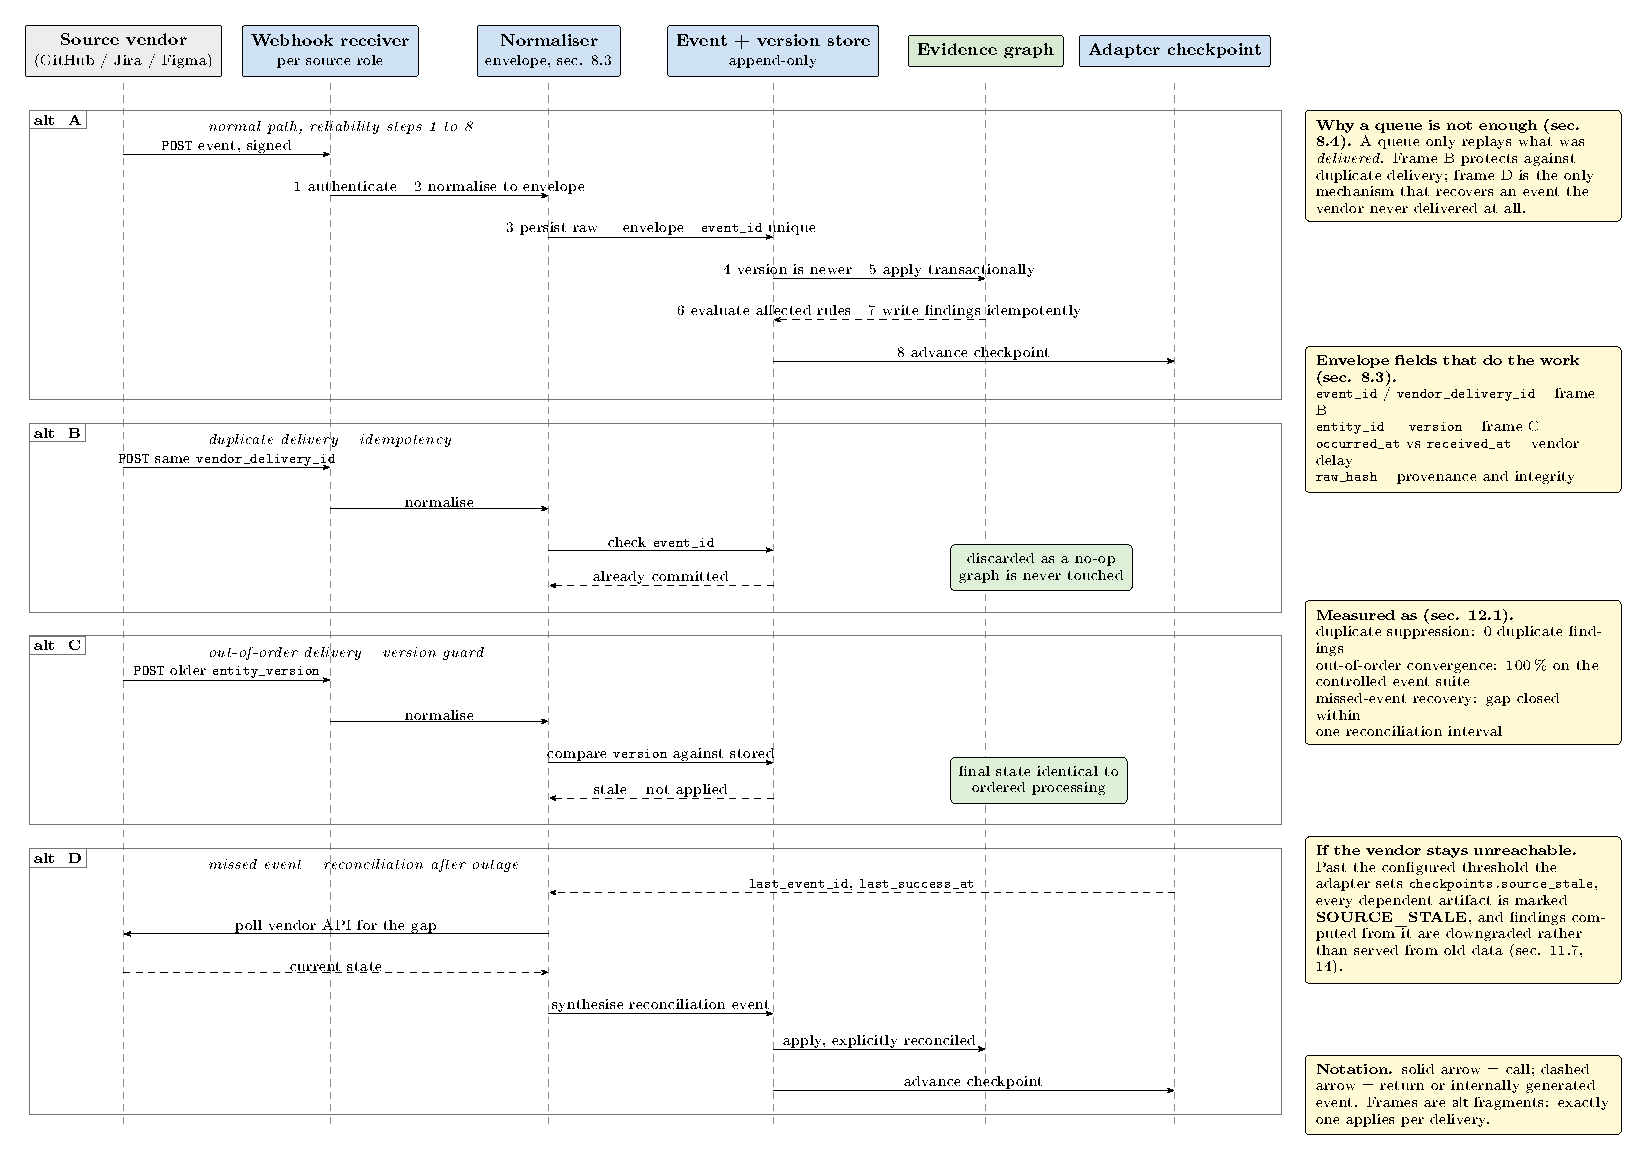
\includegraphics{diagrams/rendered/05_ingestion_sequence.pdf}}
  {Sequence diagram of source ingestion: one \textsf{alt} fragment covering
   first delivery, duplicate delivery, out-of-order delivery and missed-event
   reconciliation (proposal \S8.3--\S8.4).}
  {fig:ingestion-sequence}

\lsfigure{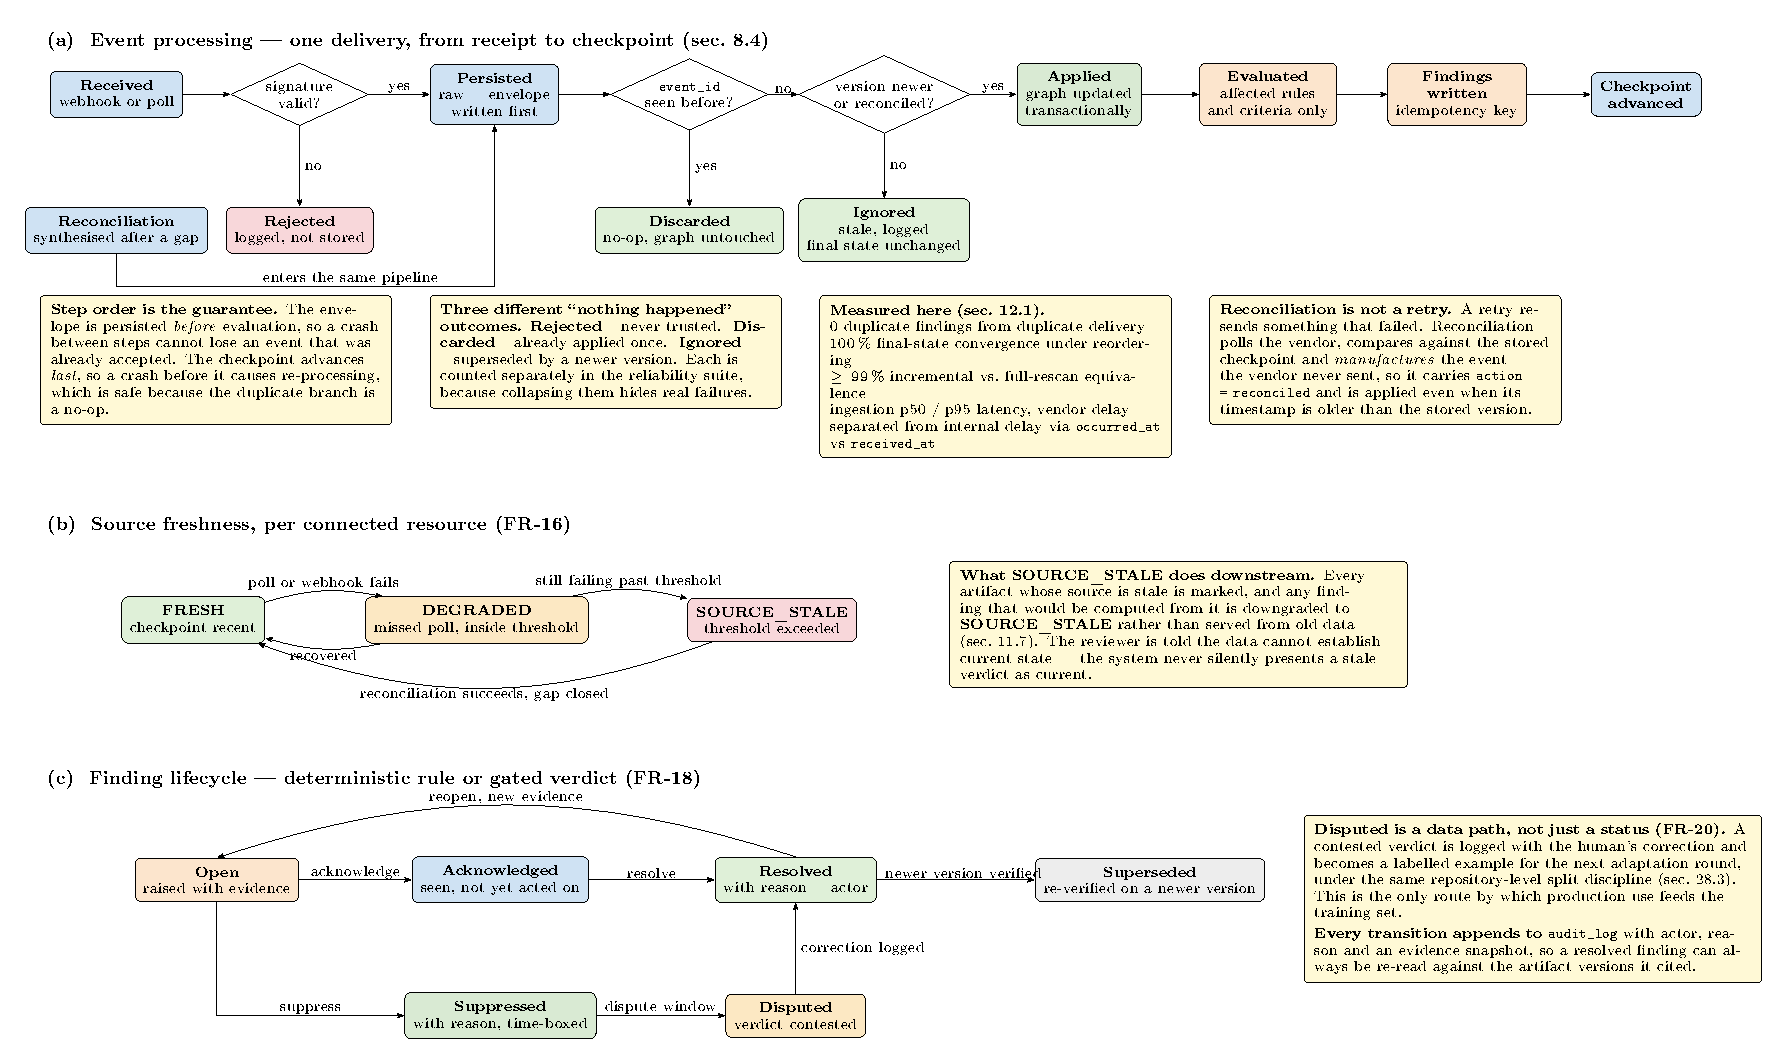
\includegraphics{diagrams/rendered/06_state_machines.pdf}}
  {State machines for (a) event processing, (b) source freshness (FR-16) and
   (c) the finding lifecycle (FR-18).}
  {fig:state-machines}

\lsfigure{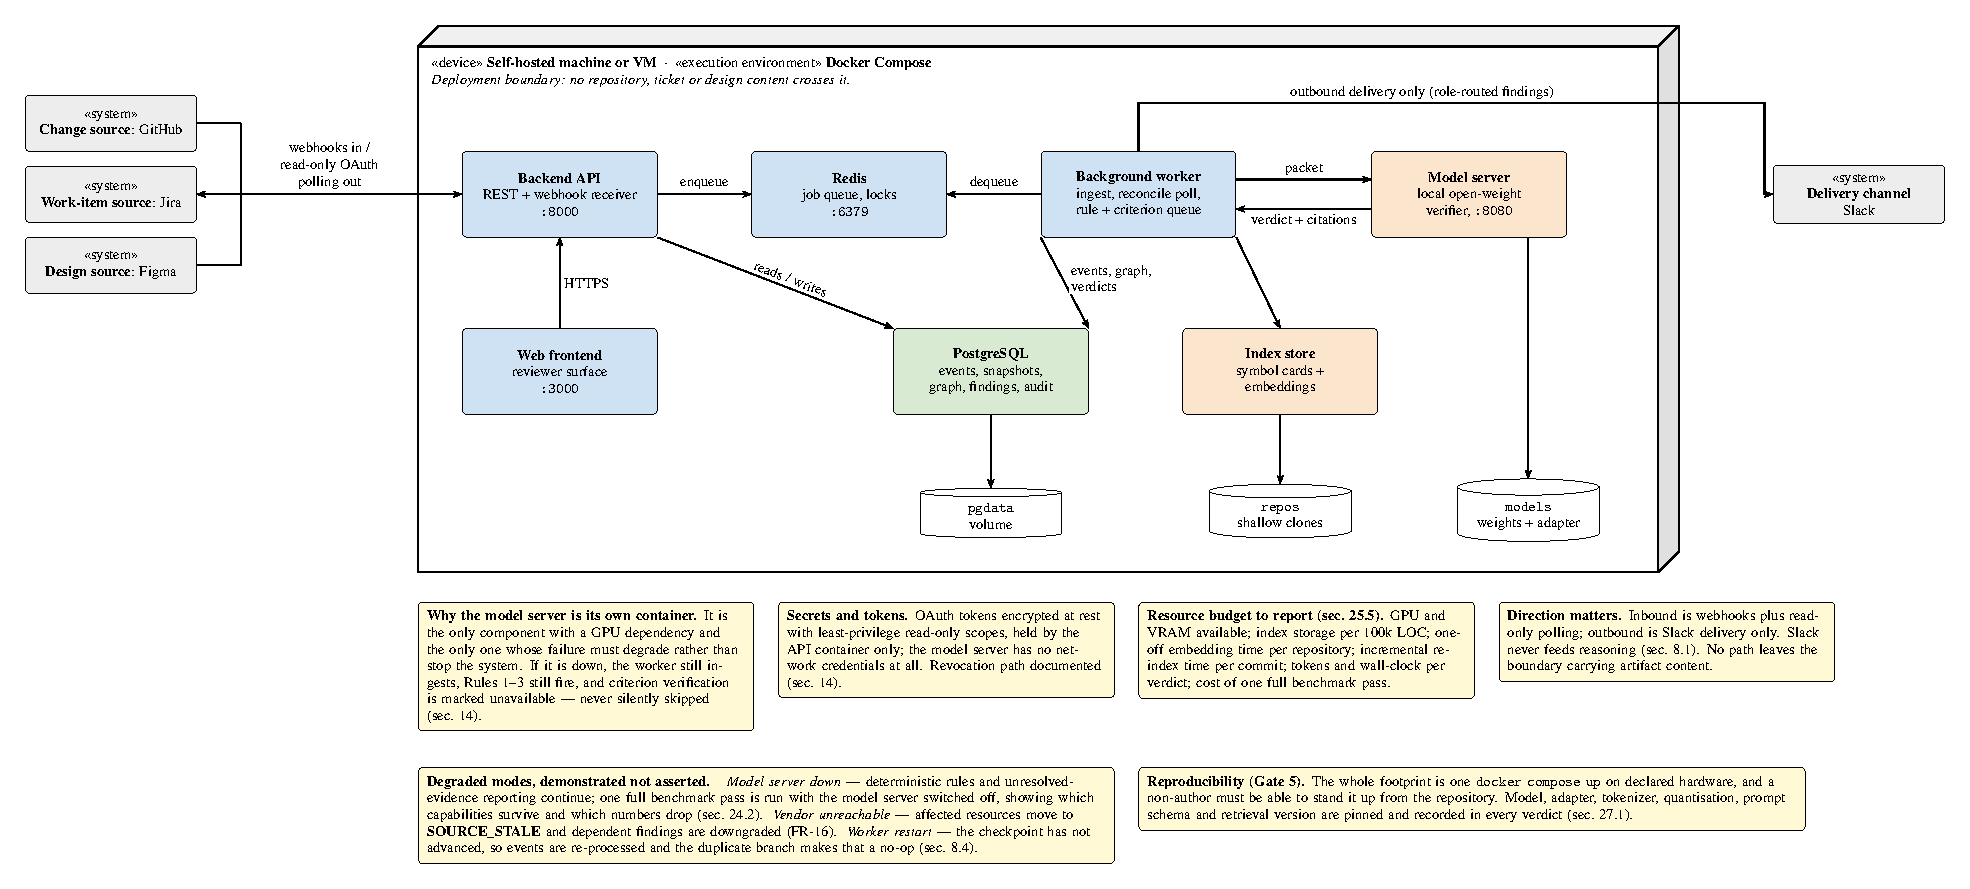
\includegraphics{diagrams/rendered/11_deployment.pdf}}
  {Deployment view: the single-host Docker Compose footprint, including the
   local model server, named volumes and the inbound/outbound boundary
   (proposal \S14).}
  {fig:deployment}

\chapter{Meeting and Progress Evidence}

\section{Progress evidence retained in the repository}

The repository does not contain formal minutes with dates and signatures.
Accordingly, this appendix records traceable progress artefacts rather than
inventing meeting attendance or decisions.

\begin{longtable}{p{0.16\textwidth}p{0.25\textwidth}p{0.43\textwidth}}
\caption{Progress and coordination evidence.}\label{tab:appendix-meetings}\\
\toprule
\textbf{Evidence} & \textbf{Purpose} & \textbf{Recorded result}\\
\midrule
\endfirsthead
\toprule
\textbf{Evidence} & \textbf{Purpose} & \textbf{Recorded result}\\
\midrule
\endhead
\texttt{TODO.md} & Work breakdown and ownership & Tracks ingestion, verifier, analyser, dataset and report tasks by owner.\\
\texttt{docs/genai\_register.md} & Tool-assisted work disclosure & Records materially assisted artefacts, review, corrections and rejected claims.\\
\texttt{docs/traceability/} & Requirement/design/code/test alignment & Generated matrix covers 43 requirements with no missing or duplicate IDs.\\
\texttt{FYP1 Mid Pre-Evaluation Student Worksheet.md} & Evaluation preparation & Records panel actions, responsibilities, demo cases, risks and individual evidence.\\
\texttt{c95df34} & Integration milestone & Adds GitHub, Jira and Figma OAuth/webhook implementation and setup evidence.\\
\texttt{a037d16} & Verification milestone & Adds the worker verifier, verdict gate and reviewer data layer.\\
\texttt{de5c1ff}, \texttt{45e5ed7} & Report-evidence milestones & Update Chapters 3, 6 and 9 using repository-backed evidence.\\
\bottomrule
\end{longtable}

\section{Supervisory follow-up register}

The panel feedback and the team's response are reproduced in
Appendix~\ref{tab:appendix-actions}. The outstanding items are model-resource
benchmarking, requirement-anchor completion, final dataset audit, live
provider rehearsal and final report/tag review. These are tracked explicitly
so a sample report does not confuse implementation evidence with supervisory
approval or a completed evaluation.

\end{document}

